\documentclass{article}



\usepackage{PRIMEarxiv}
\usepackage{natbib}


\usepackage[utf8]{inputenc} % allow utf-8 input
\usepackage[T1]{fontenc}    % use 8-bit T1 fonts
\usepackage{hyperref}       % hyperlinks
\usepackage{url}            % simple URL typesetting
\usepackage{booktabs}       % professional-quality tables
\usepackage{amsfonts}       % blackboard math symbols
\usepackage{amssymb}
\usepackage[cmex10]{amsmath}
\usepackage{nicefrac}       % compact symbols for 1/2, etc.
\usepackage{microtype}      % microtypography
\usepackage{xcolor}         % colors
\usepackage{graphicx} 
\usepackage{hyperref}
\usepackage{cleveref}
\usepackage{xr-hyper}
\usepackage{float}
\usepackage{balance}
\usepackage{mathtools}
\usepackage{bbm}
\usepackage{bm}
\usepackage{xcolor}
\usepackage{multirow}
\usepackage[size=scriptsize]{todonotes}

\usepackage[shortlabels]{enumitem}
\usepackage[normalem]{ulem}
\usepackage{pifont}% http://ctan.org/pkg/pifont
\newcommand{\cmark}{\ding{51}}%
\newcommand{\xmark}{\ding{55}}%
\usepackage{xspace}
\usepackage{diagbox}
% \usepackage[section]{placeins}

\usepackage{eqparbox,array}
\usepackage{algorithm}
\usepackage{algorithmicx}
\usepackage{algpseudocode}

\allowdisplaybreaks

\usepackage{aliascnt}
% \theoremstyle{thmstyleone}%
\newtheorem{theorem}{Theorem}%  meant for continuous numbers
%%\newtheorem{theorem}{Theorem}[section]% meant for sectionwise numbers
%% optional argument [theorem] produces theorem numbering sequence instead of independent numbers for Proposition

% \newaliascnt{proposition}{theorem}
% \newtheorem{proposition}[proposition]{Proposition}%
% \aliascntresetthe{proposition}
% \newaliascnt{corollary}{theorem}
% \newtheorem{corollary}[corollary]{Corollary}%
% \aliascntresetthe{corollary}
% \newaliascnt{lemma}{theorem}
% \newtheorem{lemma}[lemma]{Lemma}%
% \aliascntresetthe{lemma}

\newtheorem{proposition}{Proposition}% to get separate numbers for theorem and proposition etc.
\newtheorem{corollary}{Corollary}
\newtheorem{lemma}{Lemma}

% \theoremstyle{thmstyletwo}%
\newtheorem{example}{Example}%
\newtheorem{remark}{Remark}%

% \theoremstyle{thmstylethree}%
\newtheorem{definition}{Definition}
\newtheorem{assumption}{Assumption}%



\newcommand{\Real}{\mathbb{R}}
\newcommand{\AIC}{\textrm{GIC}_{\lambda_n}}
\renewcommand{\hat}{\widehat}
\renewcommand{\tilde}{\widetilde}
\def\ind{\mathbbm{1}}
\def\E{\mathbb{E}} %expectation
\def\P{\mathbb{P}} %prob
\def\T {{ \mathrm{\scriptscriptstyle T} }} %transpose
\def\var{\textit{var}} %var
\def\cov{\textit{cov}}
\def\corr{\textit{corr}}
\newcommand{\tr}{\textit{tr}}
\newcommand{\fd}{f^*}
\newcommand{\ft}{f_{N}}
\newcommand{\ul}{u}
\newcommand{\Ul}{U}
\newcommand{\pl}{\textrm{PL}}
\newcommand{\dm}{M}
\newcommand{\dmc}{\mathcal{M}}
\newcommand{\qs}{Q}
\newcommand{\qsc}{\mathcal{Q}}
\newcommand{\la}{T}
\newcommand{\lac}{\mathcal{T}}
\newcommand{\si}{\mathcal{S}}
\newcommand{\Y}{\tilde{Y}}
\newcommand{\fc}{\mathcal{F}}
\newcommand{\X}{ X}
\def\x{x}
\bmdefine\w{w}
\bmdefine\y{y}
\bmdefine\z{z}
\bmdefine\e{e}
\bmdefine\u{u}
\bmdefine\bv{v}
\bmdefine\h{h}
\bmdefine\bz{0}
\bmdefine\balpha{\alpha}
\bmdefine\bbeta{\beta}
\bmdefine\bgamma{\gamma}
\bmdefine\bmu{\mu}
\def\loss{\ell}
\newcommand{\jie}[1]{({\color{blue}#1})}
\newcommand{\gw}[1]{{\color{blue}#1}}
\newcommand{\defeq}{:=}

% \newcommand\ul{u_n}
\def\dno{\dm_{\textrm{NO}}}
\def\drn{\dm_{\textrm{IID}}}
\def\dun{\dm_{\textrm{Const}}}
\def\dour{\dm_{\textrm{Poly}}}
\def\dnt{\dm_{\textrm{Nature}}}
\def\qiid{\qs_{\textrm{IID}}}
\def\dkrr{\dm_{\textrm{KRR}}}
\DeclareMathOperator*{\dasymp}{\dot{\asymp}}
\DeclareMathOperator*{\dleq}{\dot{\lesssim}}
\DeclareMathOperator*{\dgeq}{\dot{\gtrsim}}

\def\VC{\textsc{vc}}
\def\Rad{\textsc{rad}}
\def\de{\overset{\Delta}{=}}

\renewcommand{\algorithmicrequire}{\textbf{Input:}}
\renewcommand{\algorithmicensure}{\textbf{Output:}}

\newcommand\numberthis{\addtocounter{equation}{1}\tag{\theequation}}
\newcommand{\forceindent}{\leavevmode{\parindent=1em\indent}}

\def\limp{\rightarrow_p}
\DeclareMathOperator*{\argmin}{\arg\min}
\DeclareMathOperator*{\sign}{sign}
\DeclareMathOperator*{\argmax}{\arg\max}
\DeclarePairedDelimiterX{\norm}[1]{\lVert}{\rVert}{#1}
\DeclarePairedDelimiterX{\bnorm}[1]{\biggl\lVert}{\biggr\rVert}{#1}
\DeclarePairedDelimiterX{\abs}[1]{\lvert}{\rvert}{#1}
\DeclareMathOperator*{\esssup}{ess\,sup}
\DeclarePairedDelimiterX{\ip}[2]{\langle}{\rangle}{#1,#2} % inner product

\makeatletter
\newcommand\Autoref[1]{\@first@ref#1,@}
\def\@throw@dot#1.#2@{#1}% discard everything after the dot
\def\@set@refname#1{%    % set \@refname to autoefname+s using \getrefbykeydefault
    \edef\@tmp{\getrefbykeydefault{#1}{anchor}{}}%
    \xdef\@tmp{\expandafter\@throw@dot\@tmp.@}%
    \ltx@IfUndefined{\@tmp autorefnameplural}%
         {\def\@refname{\@nameuse{\@tmp autorefname}s}}%
         {\def\@refname{\@nameuse{\@tmp autorefnameplural}}}%
}
\def\@first@ref#1,#2{%
  \ifx#2@\autoref{#1}\let\@nextref\@gobble% only one ref, revert to normal \autoref
  \else%
    \@set@refname{#1}%  set \@refname to autoref name
    \@refname~\ref{#1}% add autoefname and first reference
    \let\@nextref\@next@ref% push processing to \@next@ref
  \fi%
  \@nextref#2%
}
\def\@next@ref#1,#2{%
   \ifx#2@ and~\ref{#1}\let\@nextref\@gobble% at end: print and+\ref and stop
   \else, \ref{#1}% print  ,+\ref and continue
   \fi%
   \@nextref#2%
}
\makeatother

\makeatletter
\let\oldtheequation\theequation
\renewcommand\tagform@[1]{\maketag@@@{\ignorespaces#1\unskip\@@italiccorr}}
\renewcommand\theequation{(\oldtheequation)}
\makeatother



\def\equationautorefname{Eq.}%
\def\figureautorefname{Figure}%
\def\tableautorefname{Table}%
\def\algorithmautorefname{Algorithm}%
\def\appendixautorefname{Appendix}%
\def\sectionautorefname{Section}%
\def\subsectionautorefname{Section}%
\def\subsubsectionautorefname{Section}%
\def\theoremautorefname{Theorem}%
\def\designautorefname{Design}
\def\exampleautorefname{Example}
\def\definitionautorefname{Definition}%
\def\assumptionautorefname{Assumption}%
\def\propositionautorefname{Proposition}
\def\proofautorefname{Proof}%
\def\lemmaautorefname{Lemma}
\def\corollaryautorefname{Corollary}%
\def\remarkautorefname{Remark}
%%%%%
%% correct bad hyphenation here
\hyphenation{op-tical net-works semi-conduc-tor im-percep-tible}

%Header
\pagestyle{fancy}
\thispagestyle{empty}
\rhead{ \textit{ }} 

\title{Model Privacy: A Unified Framework to Understand Model Stealing Attacks and Defenses}


\author{
  Ganghua Wang\\
    School of Statistics \\
   University of Minnesota \\
   \texttt{wang9019@umn.edu} 
   \And
   Yuhong Yang\\
   School of Statistics \\
   University of Minnesota \\
   \texttt{yangx374@umn.edu} 
   \And
      Jie Ding \\
    School of Statistics \\
   University of Minnesota \\
   \texttt{dingj@umn.edu}
}


\begin{document}

\maketitle

\abstract{
    The use of machine learning (ML) has become increasingly prevalent in various domains, highlighting the importance of understanding and ensuring its safety. One pressing concern is the vulnerability of ML applications to model stealing attacks. These attacks involve adversaries attempting to recover a learned model through limited query-response interactions, such as those found in cloud-based services or on-chip artificial intelligence interfaces. While existing literature proposes various attack and defense strategies, these often lack a theoretical foundation and standardized evaluation criteria. In response, this work presents a framework called ``Model Privacy'', providing a foundation for comprehensively analyzing model stealing attacks and defenses. We establish a rigorous formulation for the threat model and objectives, propose methods to quantify the goodness of attack and defense strategies, and analyze the fundamental tradeoffs between utility and privacy in ML models. Our developed theory offers valuable insights into enhancing the security of ML models, especially highlighting the importance of the attack-specific structure of perturbations for effective defenses. We demonstrate the application of model privacy from the defender's perspective through various learning scenarios.  Extensive experiments corroborate the insights and the effectiveness of defense mechanisms developed under the proposed framework.
}

\keywords{Trustworthy Machine Learning, Model Attacks, Privacy, Adversarial Learning, Artificial Intelligence Security}


\section{Introduction} \label{sec:intro}
    \section{Introduction}
\label{sec:intro}

\begin{figure*}[tb]
    \centering
    \includegraphics[width=0.848\linewidth]{figs/circuitnn.pdf} 
    \caption{Illustration of differentiable CircuitNN. CircuitNN is designed based on differentiable NAND gates. After DAS is guided by PI and PO pairs of the truth table, CircuitNN can get the precise circuit architecture logic equivalent to the truth table.}
    \label{fig:circuitnn}
\end{figure*}

% 1. Describe the importance of logic synthesis
% 2. Existing Problems
% (a) Neural Architecture Search: Unstable, Predefined Setting, etc.
% (b) Circuit Generation: Probabilistic Model, Logic Equivalence

With the rapid advancement of technology, the scale of integrated circuits (ICs) has expanded exponentially. 
This expansion has introduced significant challenges in chip manufacturing, particularly concerning power and area metrics.
A primary objective in IC design is achieving the same circuit function with fewer transistors, thereby reducing power usage and area occupancy.

Logic synthesis~\cite{hachtel2005logicsynth}, a critical step in electronic design automation (EDA), transforms behavioral-level circuit designs into optimized gate-level circuits, ultimately yielding the final IC layout. 
The primary goal of logic synthesis is to identify the physical implementation with the fewest gates for a given circuit function. 
This task constitutes a challenging NP-hard combinatorial optimization problem. 
Current logic synthesis tools~\cite{brayton2010abc, wolf2013yosys} rely on human-designed heuristics, often leading to sub-optimal outcomes.

Differentiable architecture search (DAS) techniques~\cite{liu2018darts, chu2020darts} offer novel perspectives on addressing challenges in this problem.
Circuit functions can be represented through truth tables, which map binary inputs to their corresponding outputs. 
Truth tables provide a precise representation of input-output relationships, ensuring the design of functionally equivalent circuits.
Inspired by this, researchers~\cite{deepmind2024ai4sys, wang2024tnet} have begun exploring the application of DAS to synthesize circuits directly from truth tables.
Specifically, \citet{deepmind2024ai4sys} proposed CircuitNN, a framework that learns differentiable connection structures with logic gates, enabling the automatic generation of logic circuits from truth tables.
This approach significantly reduces the complexity of traditional circuit generation. 
Building on this, \citet{wang2024tnet} introduced T-Net, a triangle-shaped variant of CircuitNN, incorporating regularization techniques to enhance the efficiency of DAS.

Despite these advancements, several challenges remain. 
The computational complexity of DAS grows quadratically with the number of gates, posing scalability issues.
Although triangle-shaped architecture~\cite{wang2024tnet} partially mitigates this problem, redundancy persists. 
%Additionally, DAS is susceptible to converging to local optima, limiting the ability to search architectures that satisfy the given truth tables~\cite{liu2018darts}. 
%Furthermore, hyperparameters (network depth and layer width) require extensive searches, introducing complexity and prolonging the synthesis process. 
Additionally, DAS is susceptible to converging to local optima~\cite{liu2018darts} and hyperparameters (network depth and layer width) require extensive searches. 
The challenges arise from the vast search space in DAS. 
% Even with predefined settings for CircuitNN, finding a configuration that meets the truth table requires extensive trial and error during the DAS process. 
Intuitively, limiting the search space through predefined parameters (network depth, gates per layer, and connection probabilities) can significantly reduce the complexity.

Recent advances~\cite{openai2023gpt4, abramson2024alphafold3, esser2024sd3, li2024mar} in conditional generative models have demonstrated remarkable performance across language, vision, and graph generation tasks. 
Motivated by these developments, we propose a novel approach to circuit generation that generates preliminary circuit structures to guide DAS in generating refined circuits matching specified truth tables. 
Firstly, we introduce CircuitVQ, a tokenizer with a discrete codebook for circuit tokenization. 
Built upon our Circuit AutoEncoder framework~\cite{hou2022graphmae,li2023maskgae,wu2025mgvga}, CircuitVQ is trained through a circuit reconstruction task. 
Specifically, the CircuitVQ encoder encodes input circuits into discrete tokens using a learnable codebook, while the decoder reconstructs the circuit adjacency matrix based on these tokens.
Subsequently, the CircuitVQ encoder serves as a circuit tokenizer for CircuitAR pretraining, which employs a masked autoregressive modeling paradigm~\cite{chang2022maskgit, li2023mage}. 
In this process, the discrete codes function as supervision signals. 
After training, CircuitAR can generate discrete tokens progressively, which can be decoded into initial circuit structures by the decoder of the CircuitVQ. 
These prior insights can guide DAS in producing refined circuits that match the target truth tables precisely.

Our key contributions can be summarized as follows:
\begin{itemize}
\item We introduce CircuitVQ, a circuit tokenizer that facilitates graph autoregressive modeling for circuit generation, based on our Circuit AutoEncoder framework;
\item Develop CircuitAR, a model trained using masked autoregressive modeling, which generates initial circuit structures conditioned on given truth tables;
\item Propose a refinement framework that integrates differentiable architecture search to produce functionally equivalent circuits guided by target truth tables;
\item Comprehensive experiments demonstrating the scalability and capability emergence of our CircuitAR and the superior performance of the proposed circuit generation approach.
\end{itemize}

% Motivation
% (a) Diffusion (Vision, Graph), Autoregressive (Language, Vision)
% (b) Circuit Generation for Predefined Setting
% (c) Neural Architecture Search for Strict Logic Equivalence

% Contribution
% (a) Circuit Tokenizer (new transformer arch, training strategy)
% (b) CircuitAR (train and gen strategies, post-ar strategy)
% (c) Extensive Evaluation including BitD (Bit Distance) for Scalability


\section{Formulation of the Model Privacy Framework} \label{sec:motivation}
    \def\attstr{\textrm{AttStr}}
\def\atteff{\textrm{AttEff}}
\def\relatteff{\textrm{RelAttEff}}
\def\defstr{\textrm{DefStr}}
\def\defeff{\textrm{DefEff}}
\def\reldefeff{\textrm{RelDefEff}}
\def\utilloss{\textrm{UtilLoss}}
\def\eco{potent\xspace}


    In \Autoref{subsec:overview}, we present the background of model stealing attacks, highlighting the motivation and essential ingredients of the proposed framework. 
    In \Autoref{subsec:quantify}, we propose methods to quantify the effectiveness of attack and defense strategies with economic interpretations.
    In \Autoref{subsec:game}, we characterize the objectives and actions of both the attacker and defender, providing a foundation for theoretically analyzing the unique challenges in model privacy.


    \subsection{Background and Essential Ingredients of Model Privacy} \label{subsec:overview}
    We begin with a classical machine learning setting. Suppose a model owner has created a function $\fd$ from a large proprietary dataset to predict responses based on input $\X$. The model owner provides query-based services by responding with $\Y_i$ for any input query $\X_i$. 
    
    Meanwhile, a malicious user, or attacker, aims to build a model to either provide similar services and compete with the model owner or to discontinue paying for the service. Instead of collecting raw training data and training a model from scratch, the attacker exploits the model owner's service to significantly reduce training costs. In particular, the attacker performs a model stealing attack to reconstruct a function $\hat{f}_n$ that closely approximates $\fd$ using $n$ query-response pairs $Z_n\defeq \{(\X_i, \Y_i),i=1,\dots,n\}$. There are three essential ingredients for the attacker.
    \begin{enumerate}
        \item \textit{ Evaluation criterion} $\ell$. To evaluate the goodness of an attack, the attacker has to assess the closeness between the target function $\fd$ and the reconstructed function $\hat{f}_n$. This is measured via $\ell_A(\hat{f}_n, \fd)$, where $\ell_A$ is a loss function chosen according to the attacker's interest. For example, if the attacker wants $\hat{f}_n$ to be uniformly close to $\fd$, $\ell_A(f, g)$ could be the supremum norm $\sup_x \abs{f(x)-g(x)}$ for two functions $f$ and $g$. Alternatively, if the focus is on performance in a specific region $S$, $\ell_A(f, g)$ can be defined as $\int_{x \in S} \abs{f(x) - g(x)} dx$.
        
        \item \textit{ Attack strategy} $(\qs, \la)$. An attack strategy consists of a \textit{query strategy} $\qs$ and a \textit{learning algorithm} $\la$. The query strategy $\qs$ determines how the attacker selects $\X_i$'s. There are two types of query strategies: ``batch query'', where all $n$ queries are sent to the model owner at once, and ``sequential query'', where queries are sent one by one or in parts.
        Examples of batch query strategies include fixed designs (e.g., equally-spaced sampling over an interval) and random designs (e.g., IID sampling from a given distribution). Sequential query strategies may use previous responses to inform subsequent $\X_i$ choices. After collecting the query-response pairs $Z_n$, the attacker applies a learning algorithm $\la$ to construct $\hat{f}_n$. Common learning algorithms include linear regression, $k$-nearest neighbors, ensemble forests, and neural networks. 

        \item \textit{ Side information} $\si$.  
        Attacker's side information $\si_A$ refers to any additional information available to the attacker beyond the query-response pairs. This can include properties of the defender's model, such as knowing that $\fd$ is non-negative or is a neural network with a particular architecture, or additional data collected from other sources. Side information can enhance the attacker's learning capability.
    \end{enumerate}

    Overall, the attacker aims to choose a favorable attack strategy that allows them to accurately recover $\fd$ using a minimal number of queries.

    Given this threat, the model owner aims to prevent the attacker from easily stealing the model. As such, we name this problem as enhancing \textit{model privacy} and call the model owner the defender. There are also three key components for the defender.
    \begin{enumerate}
        \item \textit{ Evaluation criterion} $\ell$. The defender seeks to maximize the dissimilarity between $\hat{f}_n$ and $\fd$, evaluated through $\ell_D(\hat{f}_n, \fd)$. It should be noted that the defender's loss function $\ell_D$ may differ from the attacker's $\ell_A$. For example, an attacker who aims to steal a language model for a given downstream task may employ a loss function $\ell_A$ evaluated in the task-specific region $S$. Meanwhile, the defender might aim for a comprehensive defense, therefore using a different $\ell_D$ that evaluates the entire input space.

        \item \textit{ Defense mechanism} $\dm$. 
        The defender can enhance model privacy by adding perturbations to the responses, $\Y_i=\fd(\X_i)+e_i$, where $e_i$ is a perturbation determined by a defense mechanism $\dm$. Larger perturbations can increase the deviation between $\hat{f}_n$ and $\fd$. However, they also reduce the quality of service for benign users, which we refer to as \textit{utility loss}. Every defense mechanism must navigate this trade-off between privacy and utility, which is referred to as the privacy-utility trade-off.

        \item \textit{ Side information} $\si$. The defender's side information $\si_D$ refers to any knowledge about the attacker beyond the received queries. Examples include the attacker's potential query strategies and learning algorithms. This information helps the defender deploy more targeted defense mechanisms, thereby bolstering model protection.
    \end{enumerate}

    In summary, model privacy involves a competition between the attacker and defender, who engage in a non-cooperative and asymmetric interaction.


    \subsection{Goodness Quantification in Model Privacy: An Economic Perspective}\label{subsec:quantify}
        Among key ingredients identified in \Autoref{subsec:overview}, the attack strategy and defense mechanism are of most importance. This subsection provides an economic perspective on their effectiveness, offering simple and intuitive interpretations. 
        Generally speaking, for the attacker,
        % \textbf{Economic Quantification Overview:} 
        an attack strategy is considered \textit{\eco} if they can significantly reduce their cost to build a model by abusing the defender's service, compared to collecting data and training a model from scratch themselves. We illustrate this with the following example. 
        
        \begin{example}[Steal a Linear Function]\label{ex:lin}
            Suppose the defender has a linear function $\fd$ and the attacker tries to rebuild it by fitting a linear model. Without any defense mechanism, the attacker can precisely reconstruct $\fd$ with just a few query-response pairs by solving a linear equation. 
            Without querying the defender, the attacker can also collect data from nature and then build a model. The needed sample size to obtain a model $\hat{f}_n$ that is close to $\fd$, however, grows quickly as the distance between $\hat{f}_n$ and $\fd$ decreases. 
            Thus, model stealing is economically advantageous for the attacker.
        \end{example}

        We next elaborate on this idea. Let $\dnt$ denote a defense mechanism that adds perturbations such that $(\X_i,\Y_i)$'s have the same distribution as the observations collected from the nature. Let $\hat{f}_n \defeq \la(Z_n)$ denote the atacker's reconstructed function given query-response pairs $Z_n=\{(\X_i,\Y_i), i=1,\dots,n\}$ and a learning algorithm $\la$.

        % \begin{definition}[Reconstructed Function]\label{def:fhat}
        %     Given query-response pairs $Z_n=\{(\X_i,\Y_i), i=1,\dots,n\}$,  the attacker rebuilds the function $\hat{f}_n \defeq \la(Z_n)$ using a learning algorithm $\la$.
        % \end{definition}

        \begin{definition}[Necessary Stealing Sample Size] \label{def:steal_sample_size}
        The sample size needed to rebuild a function $\hat{f}_n$ that is $\epsilon$-close to $\fd$ under loss $\ell$ is defined as $n(\epsilon,\ell;\fd,\dm,\qs,\la) \defeq \inf\{n:  \E \{\ell(\hat{f}_n, \fd) \}\leq \epsilon\}$. Here, the expectation is taken over every randomness, including both the attack strategy $(\qs, \la)$ and defense mechanism $\dm$.
        \end{definition}
        
        
    \begin{definition}[Attack Strength]\label{def:atkstr}
            We define the attack strength for an attack strategy $(\qs, \la)$ with respect to the underlying function $\fd$ and defense $\dm$ as 
            \begin{align*}
            \attstr(\qs,\la \mid \fd,\dm,\ell_A) \defeq 
            \liminf_{\epsilon \to 0^+} \frac{n(\epsilon,\ell_A;\fd,\dnt,\qs,\la) \times c_{\textrm{Nature}} }{ n(\epsilon,\ell_A;\fd,\dm,\qs,\la) \times c_{\textrm{Steal}} },
            \end{align*}
            where $c_{\textrm{Nature}}, c_{\textrm{Steal}}$ are the costs of collecting a single observation from nature and the defender, respectively. An attack strategy is called \eco if $\attstr=\infty$.
    \end{definition} 

    % The interpretation of attack strength is straightforward. 
    From the attacker's perspective, attack strength is the ratio of the model reconstruction costs incurred by collecting data naturally versus by stealing from the defender.  
    It is more economical to steal the model when $\attstr > 1$, rather than collecting data independently.
    An attack with infinity strength indicates the cost of querying the defender is substantially lower compared to the cost of independent data collection. 

    In contrast to the attacker, the defender has to consider both the service quality for the benign users and the difficulty for the attacker to reconstruct $\fd$ well. 
    % the defense strength can be defined in an analogous way, measuring how many times cost the attacker has to pay by performing stealing attacks. However, preventing the attacker from rebuilding a similar model is not the only pursuit of the defender, because the defender also has to provide a reasonable service quality for general users.  
    In one extreme, suppose a defender deploys a defense of returning pure white noise. Clearly, the attacker cannot rebuild any useful model based on the defender's responses, but such a defense results in unacceptable service quality for benign users. 
    % In short, a good defense  large defense strength and limited degradation of response accuracy. 
    We thus define the utility loss of a defense $\dm$ to quantify the accuracy degradation from a benign user's perspective, and define its defense strength as follows.
    % a defense with a larger strength is considered better.
    % , which we call utility loss. 
    % A nature measure of utility loss is the average difference between perturbed response $\Y_i$ and noiseless response $\fd(\X_i)$, as defined below. 
    \begin{definition}[Utility Loss]\label{def:util}
            The utility loss of a defense mechanism $\dm$ at sample size~$n$ is defined as
            \begin{align*}
                \ul_n(\dm) \defeq \E \biggl\{ \frac{1}{n} \sum_{i=1}^n \loss_U(\fd(\X_i), \Y_i) \biggr\},
            \end{align*}
            where $\Y_i$ is determined by $\dm$ and queries, and $\loss_U$ is a loss function representing the benign users' interest. 
    \end{definition}       
    
    \begin{definition}[Defense Strength]\label{def:defstr}
        The defense strength of a defense mechanism $\dm$ with respect to $\fd$ and an attack $(\qs, \la)$ is  
        \begin{align*}
        \defstr(\dm\mid \fd,\qs,\la,\ell_D) 
                 \defeq   \liminf_{\epsilon \to 0^+} \frac{ n(\epsilon,\ell_D;\fd,\dm,\qs,\la) \times c_{\textrm{Steal}} }{n(\epsilon,\ell_D;\fd,\dnt,\qs,\la) \times c_{\textrm{Nature}} }.
        \end{align*}
        A defense mechanism $\dm$ with utility loss $\ul_n(\dm)$ is said to be \eco if $\defstr = \infty$.
    \end{definition}

    Utility loss can be understood as the average difference between the perturbed response $\Y_i$ and the noiseless response $\fd(\X_i)$. While utility loss seems to be associated with the sample size $n$, the defender can easily control it at any desired level, e.g., by scaling the magnitude of the injected perturbations. We therefore propose to only compare defense mechanisms with the same level of utility loss, and a defense with a larger strength is considered better.
    

    % Recall that a good defense mechanism $\dm$ is expected to have a large defense strength and a small utility loss. We therefore propose to only compare defense mechanisms with the same level of utility loss, and a defense with a larger strength is considered better.

    
    % It is worth mentioning that $\attstr$ and $\defstr$ are not necessary reciprocals, particularly when evaluation metrics $\ell_A$ and $\ell_D$ are distinct. 

    % Analogously, from the defender's perspective, the attacker has to spend $\defstr$ times more cost by sending queries. However, defense strength alone is inadequate for evaluating the goodness of a defense. 
    % To see it, a defense returning white noise is always \eco since it contains no useful information, but such a defense results in unacceptable service quality for benign users. Therefore, the defender aims for a defense with large defense strength and limited performance degradation, which we call utility loss. 
    % A nature measure of utility loss is the average difference between perturbed response $\Y_i$ and noiseless response $\fd(\X_i)$, as defined below. 

    
    % A good defense mechanism $\dm$ is therefore expected to have a small utility loss and a large defense strength. 
    
    
    % Lastly, we provide a concrete example of \eco attacks and defenses. 

    % \begin{example}
    %         \begin{enumerate}
    %             \item \ Linear regression with IID queries is a \eco attack strategy when there is no defense. Nevertheless, it may not be \eco if the defender adopts a defense mechanism injecting correlated noise into the response, as will be seen later in \Autoref{sec:atk}.
    %             \item \ A defense mechanism injecting a constant bias into the responses is \eco, as will be seen later in \Autoref{subsec:}.
    %         \end{enumerate}
    % \end{example}
    



    \subsection{Threat Model and Objectives of Model Privacy}\label{subsec:game}
        Building upon the essential elements and goodness quantification approach presented in previous subsections, this subsection formally states the threat model and the objectives of both the attacker and defender, completing our model privacy framework.

        \textbf{Threat Model.}
        We recall the attacker-defender interaction demonstrated in \Autoref{fig:MLaaS}. The attacker sends $n$ queries $\X_1, \ldots, \X_n$ to the defender according to a query strategy $\qs$, possibly in a sequential manner. Upon receiving the queries, the defender determines the perturbations $e_i=\dm(\X_1, \ldots, \X_i), i=1,\dots,n$ for sequential queries or $(e_1, \dots, e_n)=\dm(\X_1, \ldots, \X_n)$ for batch queries, then returns responses $\Y_i = \fd(\X_i)+e_i$ to the attacker. Here, $\dm$ is a defense mechanism, and $\fd: \mathcal{X}\to \mathcal{Y}$ is the defender's trained function that needs protection. For convenience, we assume $\mathcal{X} \in \Real^d$ and $\mathcal{Y} \in \Real$ throughout this paper, though the proposed definitions and concepts can be extended to general input and response spaces.
        Given query-response pairs $Z_n = \{(\X_i, \Y_i), i=1,\ldots,n\}$, the attacker uses a learning algorithm $\la$ to reconstruct a model $\hat{f}_n=\la(Z_n)$. Specifically, $\la$ is a measurable mapping from $Z_n$ to a measurable function of $X$. 

        \begin{remark}
        The query strategy $\qs$ is actually sample-size specific, meaning $\qs$ is a collection of finite-dimensional distributions $\{\qs_n, n=1,2,\dots\}$.  
        For batch queries, $\qs_n$ is the joint distribution of $\X_1, \dots, \X_n$. For sequential queries, $\qs_n$ can be the conditional distribution of $\X_n$ given $\X_1,\dots, \X_{n-1}$ and the responses $\Y_1,\dots,\Y_{n-1}$. 
        This creates a triangular array of random variables $\{\X_i^{(k)}, i=1,\dots, k, \ k=1,2,\dots \}$, and $\X_i$ is the abbreviation of $\X_i^{(n)}$. 
        Consequently, many quantities in model privacy can depend on $n$ and should be defined as a sequence or triangular array, such as defense mechanisms and responses. The rest of this paper mainly considers batch query strategies unless otherwise specified, thereby eliminating ambiguity related to sample size dependence.
        \end{remark}

        % \begin{table}
        %     \centering
        %     \begin{tabular}{p{0.5in}p{0.5in}p{1.1in}p{3.2in}}
        %     \toprule
        %     Type & Notion & Name & Meaning \\ 
        %     \midrule
        %      \multirow{2}{*}{Query} & $\qiid$ & IID batch query & Draws an IID sample from a given distribution \\
        %       & $\qs_{\text{ES}}$   & Equally-spaced batch query  & Draws equally-spaced points in a given area \\ \hline
        %     \multirow{3}{*}{Defense}  & $\dno$ & No defense & $e_i=0$ for $i=1,\dots,n$ \\ 
        %       &$\drn$ & IID noising & $e_i$'s are IID drawn from a distribution with zero mean \\ 
        %       &$\dun$ & Constant noising & $e_i$ is a fixed constant for $i=1,\dots,n$ \\ 
        %       &$\dnt$ & Nature noising & $e_i$'s are drawn from the natural data-generating distribution \\ 
        %         \bottomrule
        %     \end{tabular}
        %     \caption{Summary of common attack and defense strategies.}
        %     \label{tab:common_strategy}
        % \end{table}

    \textbf{Objectives.}
        Both the attacker and defender aim to make the most advantageous decisions to maximize their benefits. We denote $P_A(\qs, \la;\fd, \dm)$ as the general notion of the attacker's benefit when adopting an attack strategy $(\qs, \la)$ and facing the defender's model $\fd$ and defense mechanism $\dm$. Similarly, the defender's benefit is denoted as $P_D(\fd, \dm;\qs, \la)$. Using the cost-based goodness quantification from \Autoref{subsec:quantify} for example, the attacker's benefit can be defined as $P_A(\qs, \la;\fd, \dm) \defeq \attstr(\qs,\la\mid \fd,\dm,\ell_A)$, and the defender's benefit can take the form of $P_D(\fd, \dm;\qs, \la) \defeq \defstr(\dm \mid \fd,\qs,\la,\ell_D)\times \ind_{\ul_n(\dm) \leq U_n}$, if the defender guarantees that the utility loss level is no greater than a pre-specified constant $U_n$ for every $n$.
        
        With respect to a given $\fd$ and $\dm$, an attack strategy $(\qs^*, \la^*)$ is called the best among a collection of attacks $(\qsc, \lac)$ if
        \begin{align*}
            \qs^*, \la^* \in \argmax_{\qs \in \qsc, \la \in \lac} P_A(\qs, \la;\fd, \dm). 
            \numberthis \label{eq:best_atk}
        \end{align*}
        Analogously, with respect to an attack strategy $(\qs, \la)$, a defense mechanism $\dm^*$ is the best among a collection of defenses $\dmc$ if
        \begin{align*}
            \dm^{*} \in \argmax_{\dm \in \dmc}  P_D(\fd, \dm;\qs, \la). 
            \numberthis \label{eq:best_def}
        \end{align*}

    In summary, the threat model and objectives outlined in this subsection establish a clear framework for understanding the interaction between attackers and defenders in model privacy. By defining the key elements, such as attack strategies, defense mechanisms, and their respective benefits, we can systematically analyze and develop strategies to enhance model privacy. This framework serves as a foundation for the subsequent sections, where we delve deeper into specific strategies and their theoretical underpinnings, aiming to protect ML models from being compromised by adversarial attacks.
        





\section{Analysis via Statistical Risk} \label{sec:formulation}
    \section{Adaptive labeling as a Markov decision process} 
\label{sec:formulation}

We illustrate our formulation for model evaluation, and extend it to the ATE estimation setting at the end of the section. 
Our goal is to evaluate the performance of a prediction model $\model: \statdomain \to \mathcal \labeldomain$ over the input distribution $P_X$ that we expect to see during deployment.  Given inputs $X  \in \mc{X}$,   labels/outcomes are generated
 from some unknown function $f\opt$: $
      Y = f\opt(X) + \varepsilon$, where $\varepsilon$ is the noise.
      %~~~\mbox{where}~~\varepsilon \sim N(0, \sigma^2)
  % \begin{equation*}
  %     Y = f\opt(X) + \varepsilon~~~\mbox{where}~~\varepsilon \sim N(0, \sigma^2).
  % \end{equation*}
When ground truth outcomes are costly to obtain, previously collected labeled data $\mc{D}^0 := \{(X_i,Y_i)\}_{i \in \mc{I}}$ 
typically suffers selection bias and covers only a subset of the support of input distribution $P_X$ over which we aim to evaluate the model performance. 

Assuming we have a   pool of data $\xpool$, we design
 adaptive sampling algorithms that iteratively select
inputs in $\xpool$ to be labeled.
Since labeling inputs takes time in practice, we model
real-world instances by considering \emph{batched} settings. Our goal is to sequentially label batches of data to accurately estimate model performance over $P_X$ and therefore we assume we have access to a set of inputs $\xeval \sim P_X$. %We assume the modeler pays a fixed and equal cost for each label/outcome. 
%Our framework is general as we do not assume \xpool∼PX\xpool \sim P_X.
We use the squared loss to illustrate our framework,
where our goal is to evaluate $\E_{X \sim P_X}[ (Y - \model(X))^2]$. Under the ``likelihood" function $p(y | f, x) = p_{\varepsilon}(y - f(x))$,  let $g(f)$ be the performance of the AI model $\model(\cdot)$ under the  data generating function $f$, which we refer to as our estimand of interest.
When we consider the mean squared loss,  $g(f)$ is given by 
\begin{align}
    g(f) \defeq \E_{X \sim P_X}\left[ \E_{Y \sim p(\cdot|f,X) } \Big[ (Y - \model(X))^2 \Big] \mid f \right]. \label{eqn:l2-g-f}
\end{align}
Our framework is general and can be extended to other settings. For example, a clinically useful  metric is \texttt{Recall}, defined as the fraction of individuals that the model $\model(\cdot)$ correctly labels as positive  among all the individuals who actually have the positive label 
\begin{align*}
    g(f) \defeq  \E_{X \sim P_X}\left[ \E_{Y \sim p(\cdot|f,X) } \Big[\indic{\model(X)>0}|Y=1\Big] \mid f\right].
\end{align*}
 
  Since the true function $f\opt$ is unknown, we  model it from a Bayesian perspective by formulating a posterior given the available supervised data. We refer to uncertainty over the data generating function $f$ as \emph{epistemic} uncertainty---since we can resolve it with more data---and that over
 the measurement noise $\varepsilon$ as \emph{aleatoric} uncertainty. 
Assuming independence given features $X$, we model the  likelihood of the data via the product 
$p({Y}_{1:m}|f, {X}_{1:m}) = \prod_{i=1}^m p(Y_i|f,X_i)$.
 Our prior belief  $\mu$ over functions $f$   reflects our uncertainty about how
labels are generated given features. 
To adaptively label inputs from $\mc{X}_{\rm pool}$, we assume access to an uncertainty quantification (UQ) method that provides posterior beliefs $\mu(f \mid \mc{D})$ given
any supervised data $\mc{D}:= \{(X_i,Y_i)\}_{i \in \mc{I}}$. As we detail  in Section~\ref{sec:uq}, our framework can leverage both classical 
Bayesian models like Gaussian processes and recent advancements in deep learning-based UQ  methods.

As new batches are labeled, we update our posterior beliefs about $f$ over time, which we view as ``state transitions'' of a dynamical system.
Recalling the Markov decision process depicted in Figure~\ref{fig:overview}, we sequentially label a batch of inputs from $\mc{X}_{\rm pool}$ (actions), which lead to state transitions (posterior updates).
Specifically, our initial state is given by $\mu_0(\cdot) = \mu(\cdot \mid \mc{D}^0)$, where $\mc{D}^0$ represents the initial labeled dataset.
At each period $t$, we label a batch of $K_t$ inputs $\mc{X}^{t+1} \subset \mc{X}_{\rm pool}$ resulting in labeled data $ \mc{D}^{t+1} = (\mc{X}^{t+1}, \datay^{t+1})$. After acquiring the labels at each step $t$, we update the posterior state to $\mu_{t+1}(\cdot) = \mu_t(\cdot \mid \mc{D}^{t+1})$. Modeling practical instances, we consider a small horizon problem with limited adaptivity $T$. Formulating an MDP over posterior states has long conceptual roots, dating back to the Gittin's index for multi-armed bandits~\citep{Gittins79}.

 We denote by $\pi_t$ the adaptive labeling policy at period $t$. We account for randomized policies $\datax^{t+1} \sim \pi_t(\mu_t)$ with a flexible batch size $|\datax^{t+1}| = \batchsize_t$.   
We assume $\pi_t$ is $\mc{F}_t-$measurable for all $t < T$, where $\mc{F}_t$ is the filtration generated by the observations up to the end of step $t$.
 Observe that $\mu_{t+1}$ contains randomness in the policy $\pi_t$ as well as randomness in $\datay^{t+1} \mid (\datax^{t+1},\mu_t)$. Letting $\pi = \set{\pi_0,....,\pi_{T-1}}$,  we minimize the uncertainty over $g(f)$
 at the end of data collection
\begin{align}
H(\pi) \defeq \E_{\mc{D}^{1:T} \sim \pi} \left[G(\mu_{T}) \right]  \defeq  \E_{\mc{D}^{1:T} \sim \pi} \left[G(\mu(\cdot \mid \mc{D}^{0:T})) \right]
%\defeq \E_{\mc{D}^{1:T} \sim \pi} \left[ \V_{f \sim \mu_{T}}  g(f)  \right]
     = \E_{\mc{D}^{1:T} \sim \pi} \left[ \V_{f \sim \mu(\cdot \mid \mc{D}^{0:T})}  g(f)  \right],
     \label{eqn:general-obj}
\end{align}   
where $G(\mu_T) = \V_{f \sim \mu_T}  g(f)$.
In the above objective~\eqref{eqn:general-obj}, we assume
that the modeler pays a fixed and equal cost for each outcome. 
Our framework can also seamlessly accommodate variable labeling cost. Specifically, we can define a cost function $c(\cdot)$ 
 applied on the selected subsets 
 and update the objective~\eqref{eqn:general-obj} accordingly to include the term  $\lambda c(\mc{D}^{1:T})$,
 where $\lambda$
 is the penalty factor that controls the trade-off between minimizing variance and cost of acquiring samples.


Our framework can be easily extended to causal estimation problems.  Consider a feature vector ${X}$ and suppose we have two treatment arms $Z \in \{0,1\}$. Our objective is to evaluate the average treatment effect over the population distribution $P_X$.  Given feature vector $X$, and treatment $Z$,  outcomes are generated from an unknown function $f\opt$: 
$Y = f\opt(X,Z) + \varepsilon.$
%~~~\mbox{where}~~\varepsilon \sim N(0, \sigma^2)
  % \begin{equation*}
  %     Y = f\opt(X) + \varepsilon~~~\mbox{where}~~\varepsilon \sim N(0, \sigma^2).
  % \end{equation*}
The available data is denoted by $\mc{D}^0 := \{X_i,Y_i,Z_i\}_{i \in \mc{I}}$ and given a pool of candidates 
$\xpool$, we want an
 adaptive sampling algorithms that iteratively select
candidates in $\xpool$ to be assigned a random treatment so that we can estimate average treatment effect efficiently. Under the ``likelihood" function $p(y | f, x, z) = p_{\varepsilon}(y - f(x,z))$,  let $g(f)$ represent  the average treatment effect, which is our estimand of interest. Formally, this is expressed as:
\begin{align}
g(f) \defeq \E_{X \sim P_X} \left[\E_{Y_1 \sim p(\cdot|f,X,Z=1) , Y_0 \sim p(\cdot|f,X,Z=0)} \left[Y_1 -  Y_0 \right]\mid f \right]. \label{eqn:ate-g-f}
\end{align}




 %Again the true function $f\opt$ is unknown and we model it from a Bayesian perspective by formulating a posterior  given available data.
 Our prior belief  $\mu$ over functions $f$, now 
 reflects our uncertainty about how
outcomes are generated given features and treatments. 
  We sequentially observe outcome of a batch of inputs from $\mc{X}_{\rm pool}$ (actions), and treatments assigned to this batch. We assume that selected batch of inputs $\mc{X}^t$ is randomly assigned treatments $\mc{Z}^t$ with each $Z\sim p_Z$. We summarize our formulation in Figure~\ref{fig:MDP_framework_flowchart}.
%Specifically, our initial state is given by $\mu_0(\cdot) = \mu(\cdot \mid \mc{D}^0)$ and at each period $t$, we get outcomes for a batch of $K$ candidates $\mc{X}^{t+1} \subset \mc{X}_{\rm pool}$, with randomly assigned treatments $\mc{Z}^{t+1}$ (with each $Z\sim p_Z$) and get the data $ \mc{D}^{t+1} = (\mc{X}^{t+1} \times \datay^{t+1} \times \mc{Z}^{t+1} )$. After acquiring the data at each step $t$ we update posterior state to $\mu_{t+1}(\cdot) = \mu_t(\cdot \mid \mc{D}^{t+1})$. Modeling practical instances, we consider a small horizon problem with limited adaptivity $T$.  We denote by $\pi_t$ the adaptive labeling policy at period $t$. We account for randomized policies $\datax^{t+1} \sim \pi_t(\mu_t)$ with a flexible batch size $|\datax^{t+1}| = \batchsize_t$.   
Again, we assume $\mu_t$ is $\mc{F}_t-$measurable for all $t < T$, where $\mc{F}_t$ is the filtration generated by the observations up to the end of step $t$.
 Observe that $\mu_{t+1}$ contains randomness in the policy $\pi_t$, randomness in treatment assignment $\mc{Z}^{t+1}$ and randomness in $\datay^{t+1} \mid (\datax^{t+1}, \mc{Z}^{t+1},\mu_t)$. Letting $\pi = \set{\pi_0,....,\pi_{T-1}}$,  we minimize the uncertainty over $g(f)$
 at the end of data collection:
\begin{align}
\E_{\mc{D}^{1:T} \sim \pi} \left[G(\mu_{T}) \right] \defeq
\E_{\mc{D}^{1:T} \sim \pi} \left[ \V_{f \sim \mu_{T}}  g(f)  \right]
= \E_{\mc{D}^{1:T} \sim \pi} \left[ \V_{f \sim \mu(\cdot \mid \mc{D}^{0:T})}  g(f)  \right].
\label{eqn:general-ate-obj}
\end{align}  


 

\begin{figure}[ht]
\centering
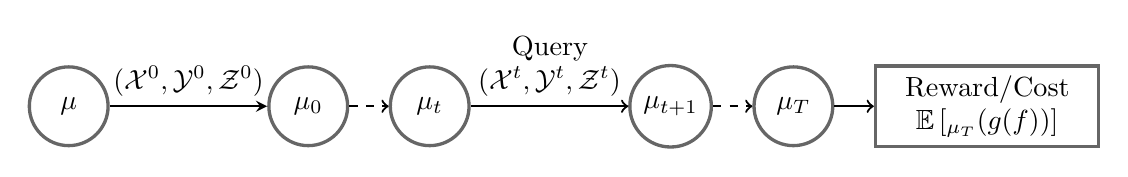
\begin{tikzpicture}
[
roundnode/.style={circle, draw=black!60, very thick, minimum size=10mm},
squarednode/.style={rectangle, draw=black!60, very thick, minimum size=10mm, align =center,text width = 26mm},
]
%Nodes
\node[roundnode]      (maintopic)                              {$\mu$};
\node[roundnode]        (circle1)       [right=20mm of maintopic] {$\mu_0$};
\node[roundnode]      (circle2)       [right=5mm of circle1] {$\mu_t$};
\node[roundnode]        (circle3)       [right=20mm of circle2] {$\mu_{t+1}$};
\node[roundnode]        (circle4)       [right=5mm of circle3] {$\mu_T$};
\node[squarednode]        (circle5)       [right=5mm of circle4] {Reward/Cost $\E \left[ \V_{\mu_T} (g(f))\right]$};


%Lines
\draw[thick, ->, >=stealth] (maintopic.east) -- node[anchor=south] {$(\mathcal{X}^0,\mathcal{Y}^0,\mathcal{Z}^0)$} (circle1.west);
\draw[thick, ->, dashed] (circle1.east) --  (circle2.west);
\draw[thick, ->] (circle2.east)  -- node[above, align =center, text width = 18mm] { Query $(\mathcal{X}^t,\mathcal{Y}^t,\mathcal{Z}^t)$} (circle3.west);
\draw[thick, ->,dashed] (circle3.east) --  (circle4.west);
\draw[thick, ->] (circle4.east) --  (circle5.west);


\end{tikzpicture}
\caption{MDP framework for adaptive labeling to efficiently estimate the average treatment effect (ATE).}
\label{fig:MDP_framework_flowchart}
\end{figure}
 









\begin{comment}
\subsection{Broader applicability of the framework to other problem settings} \label{sec:broad-framework-accuracy}
 

Although  we describe our setting in a healthcare setting with the objective  to estimate the recall of a trained AI model $\model(\cdot)$, the framework caters to many other problem settings. The extension to the evaluation of model based on accuracy (in regression setting) is straightforward, we simply replace the definition of recall $g(f)$ in~\eqref{eqn:l2-g-f} with
\begin{align*}
    g(f) = \E_{\substack{ y \sim p(y|f,x) \\  \forall x \in \mathcal X}} \big( \E_{{\textbf x} \sim p_x} [y-\model(x)]^2 \big).
\end{align*}


\textcolor{red}{To discuss if we need to have it here}
We can also extend this setting to the efficient estimation of the ATE as well. We describe these in detail below:

\begin{itemize}
    
    \item Estimating accuracy:  \[g(f) = \E_{\substack{ y \sim p(y|f,x) \\  \forall x \in \mathcal X}} \big( \E_{{\textbf x} \sim p_x} [y-\model(x)]^2 \big)\]
%    \item Estimating ATE with known control arm: 
%\[g(f) = \E_{\substack{ y \sim p(y|f,x) \\  \forall x \in \mathcal X}} \big( \E_{{\textbf x} \sim p_x} [y-\model(x)] \big)\]
\item Estimating ATE  (with minor modifications - broad structure remains similar) : 


Consider feature vector ${\mathbf x} \in \mathcal X $  distributed as ${\mathbf x}  \sim p_{\mathbf x}$, treatment $z \in {\mathcal Z} = \{0,1\}$, and a class of random functions $f: {\mathcal X} \times {\mathcal Z} \to {\mathcal Y}$, which determines the likelihood $p(y_i|f,{\mathbf x_i},z_i)$. Note that $f$ is random and reflects our uncertainty about how
labels are generated given features and the treatment. Additionally, the joint likelihood is determined as follows,  

\[p(Y|f,X,Z) = \prod_{i} p(y_i|f,{\mathbf x_i}, z_i) \]

Assuming the prior over functions $f$ to be $\mu$, therefore we have 
\[p(Y|X,Z) = \int \prod_{i} p(y_i|f,{\mathbf x_i},z_i) d\mu(f) \]


Also, assuming that under the  true data generating function $f$ (if known precisely - which we don't), the estimand of interest is

\[ \E_{{\textbf x} \sim p_x}  \left( \E_{\substack{ y \sim p(y|x,f,z=1) }} y - \E_{\substack{ y \sim p(y|x,f,z=0) }} y \right) \]


Throughout the paper we assume the above data generating process.  Now, suppose we have some labeled  data $(\datax^0,\datay^0,Z^0) =({\mathbf x}_{1:m}^0,y_{1:m}^0, z_{1:m}^0)$. 
    We run a experiment, in which we want to query the labels (in batches), so as to minimize the uncertainty of the estimand of interest. Suppose, the horizon of the experiment is $T$. Now, given prior $\mu$ and labeled data $\datax^0,\datay^0,Z^0$, in the beginning of our experiment the posterior state is $\mu_0$.

 At each step $j$ ($j \geq 1$), we query labels for a batch (with size $k$) of unlabeled data $(\datax^j,Z^j) \subset \mathcal X \times \mathcal Z$  and get labels $\datay^j$. After acquiring the labels at each step $j$ we update posterior state to $\mu_{j+1}$, informed by $\mu_j$ and $(\datax^j,\datay^j,Z^j)$. 
 
 Let the policy at step $j$ be $\pi_j$ (potentially random), which gives $\datax^{j+1},Z^{j+1} \sim \pi_j(\mu_j)$.  Observe that $\mu_{j+1}$ is random because of the randomness of the policy $\pi_j$ and $\datay^{j+1}|\{\datax^{j+1},Z^{j+1},\mu_j\}$ (\textcolor{red}{can this be written in a better way?}). Let, $\pi = \{\pi_0,....,\pi_{T-1}\}$. Therefore, our objective is to

 
\[ \min_{\pi} \E \left[ {\mathbf {Var}}_{f \sim \mu_T} \left( \E_{{\textbf x} \sim p_x}  \left( \E_{\substack{ y \sim p(y|x,f,z=1) }} y - \E_{\substack{ y \sim p(y|x,f,z=0) }} y \right) \right) \right]\]

where, $\mu_T$ depends on $\{(\datax^i,\datay^i,Z^i)\}_{i=0}^T$ and outer expectation is over both $\pi$ and  $\datay^{j+1}|\{\datax^{j+1}, Z^{j+1},\mu_j\}$ for all $j \in [0,T-1]$.


%Constraining the action space is straightforward - by first choosing set of x's using k-subset and then assigning treatment with learnable probability parameters $w_1,...,w_n$.

\end{itemize}

 \[ g(f) = \E_{\substack{ y \sim p(y|f,x) \\  \forall x \in \mathcal X}}\E_{{\textbf x} \sim p_x} g(y,{\textbf x}) \approx \E_{\substack{ y \sim p(y|f,x) \\  \forall x \in  \datax^u}} \left( \frac{1}{n}\sum_{i=1}^n \tilde{g}(y,{\textbf x}_i^u) \right)\]




Notation borrowed from a combination of the following papers 
~\citep{LeeYuNaFoLe23, KatoOgKoIn24, FongHoWa24}

%  
\end{comment}


%%% Local Variables:
%%% mode: latex
%%% TeX-master: "main"
%%% End:


\section{Defending against a Known Attack Learning Algorithm} \label{sec:model_func}
    \begin{table}[ht!]
\centering
\caption{\textbf{Super Resolution Performance Results.} Our proposed WGAN EEG Spatial Upsampling method significantly outperforms a baseline of Bicubic Interpolation commonly used in EEG upsampling pipelines.}
\label{tab:results}
\resizebox{0.8\linewidth}{!}{%
\begin{tabular}{@{}cccccc@{}}
\toprule
\multirow{2}{*}{\textbf{Dataset}} & \multirow{2}{*}{\textbf{Scale}} & \multicolumn{2}{c}{\textbf{Bicubic}} & \multicolumn{2}{c}{\textbf{WGAN}} \\ \cmidrule(l){3-6} 
                      &   & \textbf{MSE} & \textbf{MAE} & \textbf{MSE}    & \textbf{MAE}   \\
\toprule
\multirow{2}{*}{Val}  & 2 & 3.71E7       & 3.89E3       & \textbf{2.01E3} & \textbf{24.38} \\
                      & 4 & 7.23E7       & 6.42E3       & \textbf{8.53E3} & \textbf{63.83} \\
\midrule
\multirow{2}{*}{Test} & 2 & 3.75E7       & 3.91E3       & \textbf{2.06E3} & \textbf{24.66} \\
                      & 4 & 7.30E7       & 6.45E3       & \textbf{8.68E3} & \textbf{64.39} \\
\bottomrule
\end{tabular}%
}
\end{table}
        
\section{Defending against an Unknown Attack Learning Algorithm} \label{sec:atk}
    
In this section, we study the defense against an attacker whose learning algorithm is unknown to the defender. Specifically, the attacker's learning algorithm collection $\lac$ includes any measurable mappings from query-response pairs to a measurable function of $\X$. Our results address the minimum guaranteed privacy level provided by three defense mechanisms.
As a demonstrative application of the developed theory, we make the following assumption in this section, and all proofs are included in Appendix.

\begin{assumption}[H\"{o}lder function class] \label{asmp:func}
    The defender's function $\fd$ belongs to a H\"{o}lder class $\fc \defeq \hld(C,\alpha)$ with $C>0$ and $\alpha>0$.
    % , and $\norm{\fd}_{\infty} < B$ for some constant $B>0$. 
\end{assumption}


\subsection{IID Noising Defense}
    We first study the IID Noising defense $\drn$, where the defender adds IID Gaussian noise with a common variance $\sigma_n^2$
    % \todo{may extend to other distribution than Gaussian} 
    to the responses. Its privacy level against an arbitrary attacker is derived as follows.

     \begin{theorem} % [H\"{o}lder class, IID noise]
     \label{ex:holderIID}
        Under \Autoref{asmp:same_query, asmp:bounded_input, samp:density, asmp:func},
        we have
        \begin{align*}
            \pl_n(\drn,\fc\mid\qiid,\lac) \begin{cases} 
            \asymp  (\sigma_n^2/n)^{2\alpha/(2\alpha+d)}, & \sigma_n^2 \gtrsim n^{-2\alpha/d} \\ 
            \lesssim n^{-2\alpha/d} , & \sigma_n^2 \lesssim n^{-2\alpha/d}.
            \end{cases}
        \end{align*}
    \end{theorem}

    Notably, \Autoref{ex:holderIID} \textit{allows the noise variance $\sigma_n^2$ to vanish}. When the noise variance is fixed, the privacy level can be analyzed using classical minimax theory. However, the case where $\sigma^2_n \to 0$ as $n \to \infty$ has received little attention in the existing literature. Gaining an understanding of this case is crucial for model privacy, as a defense with vanishing noise can still be \eco, meaning that the attacker cannot steal a good model while the benign users' service quality is well maintained. Technically, to handle the case with vanishing noise, we need to derive the exact convergence rates of prediction error brought by randomness in queries and perturbations, respectively. 

    The privacy level derived in \Autoref{ex:holderIID} also yields the limit of the attacker's stealing error since we assumed that the attacker and the defender use the same loss, as discussed in \Autoref{sec:formulation}. For instance, under the IID Noising defense with $\sigma_n^2 \gtrsim n^{-2\alpha/d}$, an attacker uses $k$-NN can achieve the smallest stealing error at the order of $(\sigma_n^2/n)^{2\alpha/(2\alpha+d)}$. 

    % \begin{remark}[Vanishing noise]
    %     When the noise variance, $\sigma_n^2$, is fixed at $\sigma^2 > 0$, the privacy level $\pl_n$ can be analyzed using classic minimax theory. 
    %     In contrast, the case where $\sigma^2_n \to 0$ as $n \to \infty$ has received little attention in the existing literature. Gaining an understanding of this situation is crucial for model privacy, as a defense with diminishing noise can still remain \eco. As a result, the attacker cannot steal a good model while the benign users' service quality is largely preserved.
    % \end{remark}

    
   

    % \begin{remark}[General stealing limit with IID noise]
    %     We derive the following bounds on the stealing limit for a general function class $\fc$. Denote $\epsilon$-packing entropy as $S(\epsilon)$ and $\epsilon$-covering entropy as $V(\epsilon)$ \citep[see, e.g.][]{yang1999information}. 
    %     \begin{assumption}\label{asmp:atk_iid}
    %         1. $\fc$ is rich, that is, $\liminf_{\epsilon \to 0^+}S(\alpha\epsilon)/S(\epsilon) > 1$ for some $\alpha \in (0,1)$. 2. There exist positive constants $a$, $b$, and $c$ such that $S(\epsilon) \leq V(b\epsilon) \leq cS(\alpha\epsilon)$ when $\epsilon$ is sufficiently small. 
    %         3. The noise variance $\sigma_n^2 \lesssim 1$.
    %     \end{assumption}
    %         \begin{theorem}[General function class, IID noise]\label{thm:atk_iid}
    %         Let $\epsilon_n$ and $\underline{\epsilon}_n$ be such that
    %         \begin{align*}
    %             n\epsilon_n^2 = V(\epsilon_n), \quad n\underline{\epsilon}_n^2/\sigma_n^2 = V(\underline{\epsilon}_n).
    %         \end{align*}
    %         Under \Autoref{asmp:atk_iid}, we have $\underline{\epsilon}_n^2 \lesssim R_n \lesssim \epsilon_n^2$. 
    %             In particular, if $\sigma_n^2 \asymp 1$, we have $R_n \asymp \epsilon_n^2$, and the attacker can construct a learning algorithm $\la^*$ to achieve this rate.
    %         \end{theorem}
            
    %         \Autoref{thm:atk_iid} implies that $\underline{\epsilon}_n = o(\epsilon_n)$ as $\sigma_n^2 \to 0$, leading to a gap between the lower and upper bounds. 
    %         % Though we derive the exact minimax rate in \Autoref{ex:holderIID}, 
    %         It is generally unclear whether this gap can be closed, and we leave it for future work. 
    % \end{remark}
    
    

    % \begin{remark}[Query strategy matters, I]
    \Autoref{ex:holderIID} assumes that the attacker adopts an IID batch query strategy. 
    % We can prove that IID batch query is indeed optimal for the attacker. 
    The following theorem implies that in this regression task, IID batch query is the best choice for the attacker when $\sigma_n^2 \gtrsim n^{-2\alpha/d}$.
    
        \begin{theorem}[Non-IID Queries]\label{thm:IIDquery}
         Under \Autoref{asmp:same_query, asmp:bounded_input, samp:density, asmp:func}, we have $\pl_n(\drn,\fc\mid \qs,\lac) \gtrsim (\sigma_n^2/n)^{2\alpha/(2\alpha+d)}$ for every query strategy $\qs$. 
        \end{theorem}    
        % For any $p>0$, we denote the $\epsilon$-covering entropy of the function class $\mathcal{F}$ under $L_p$ loss as $V_p(\epsilon)$ \citep[see, e.g.][]{yang1999information}. 
        % \begin{assumption}\label{asmp:atk_iid}
        %     1. $\fc$ is rich, that is, $\liminf_{\epsilon \to 0^+}S(\alpha\epsilon)/S(\epsilon) > 1$ for some $\alpha \in (0,1)$. 2. There exist positive constants $a$, $b$, and $c$ such that $S(\epsilon) \leq V(b\epsilon) \leq cS(\alpha\epsilon)$ when $\epsilon$ is sufficiently small. 
        %     3. The noise variance $\sigma_n^2 \lesssim 1$.
        % \end{assumption}
        


        % Let $R_n(\qiid)$ and $R_n(\qs)$ denote the stealing limit with respect to IID batch query strategy and an arbitrary query strategy $\qs$, respectively.
        % Let $\pl_n(\drn,\fc\mid \qs,\lac)$ denote the privacy level of $\drn$ under an arbitrary query strategy $\qs$.
        % \begin{align*}
        %     R_n(\fc,\dmc,\qiid,\lac) \asymp R_n(\fc,\dmc,\qsc,\lac).
        % \end{align*}
        % Compared to \Autoref{ex:holderIID}, \Autoref{thm:IIDquery} implies that in this regression task, an attacker using IID batch query achieves the best stealing error rate when $\sigma_n^2 \gtrsim n^{-2\alpha/d}$.
        % However, the choice of query strategy has to be carefully considered for classification tasks, and IID query strategy is typically suboptimal in this case. In particular, the behavior of a classifier near the decision boundary is most critical, thus the attacker may pay more attention to those areas. \todo{Need support, using logistic example or simply cite some work?}
        
        
    % \end{remark}

    \subsection{Correlated Noising Defense}\label{subsec:corr_noise}
    Using an IID Noising defense mechanism is often insufficient to prevent model stealing attacks. To enhance protection, the defender can add noise with correlation.
    One such choice is adding stationary noise with variance $\sigma_n^2$. The correlation structure of noise is characterized by $r(\abs{i-j})\defeq\corr(e_i,e_j)$, where $e_i$ is the perturbation added to the $i$-th response. For example, $r(k)=\ind_{k=0}$ corresponds to an IID Noising defense mechanism $\drn$, $\sum_{k=0}^\infty \abs{r(k)} < \infty$ represents short-range dependent noise, and $r(k) \asymp k^{-\gamma} $ with $ 0<\gamma<1,$ is a typical example of long-range dependent noise. \Autoref{ex:hld_longrange} analyzes the privacy level of adding long-range dependent noise.

   \begin{theorem}% [H\"{o}lder class, long-range dependent noise]
    \label{ex:hld_longrange}
        Let $\dm_{\gamma}$ represent a defense mechanism that adds long-range dependent noise with $r(k)\asymp k^{-\gamma}$ for some $\gamma \in (0,1)$ and $ \ul_n(\dm_{\gamma}) = \sigma_n^2$. 
        Under \Autoref{asmp:same_query, asmp:bounded_input, samp:density, asmp:func}, we have 
        \begin{align*}
            \pl_n(\dm_{\gamma},\fc\mid \qiid,\lac)  \begin{cases} 
            \asymp (\sigma_n^2/n)^{2\alpha/(2\alpha+d)}+\sigma_n^2n^{-\gamma}, & \sigma_n^2 \gtrsim n^{-2\alpha/d} \\ 
            \lesssim n^{-2\alpha/d} , & \sigma_n^2 \lesssim n^{-2\alpha/d}.
            \end{cases}
        \end{align*}
    \end{theorem}

    \Autoref{ex:hld_longrange} demonstrates that the correlation structure of noise can be tailored to impede the attacker's ability to learn the defender's model effectively. Compared to \Autoref{ex:holderIID}, adding long-range dependent noise instead of IID noise can significantly increase privacy level. Moreover, a stronger correlation (a smaller $\gamma$) in the noise leads to a higher privacy level. 
    

    \begin{remark}[Influence of Query Strategy]
        In the context of \Autoref{ex:hld_longrange}, \citet{hall1990nonparametric, wang1996function} showed that $\pl_n(\dm_{\gamma},\fc\mid \qs,\lac) \asymp n^{-2\alpha\gamma/(2\alpha+\gamma)}$ when $\qs$ is an equally-spaced fixed design, $\sigma_n^2 \asymp 1$, and $\X$ is one-dimensional. This rate is slower compared to using an IID batch query. As a result, when the attacker uses a batch query strategy, the defender can add long-range dependent noise in the order of $X_i$'s values to hinder the attacker's ability to learn $\fd$. In contrast, if the attacker adopts a sequential query strategy that requests immediate responses, the defender can only add long-range noise in the order of queries, potentially allowing the attacker to learn $\fd$ at a faster rate of convergence. 
    \end{remark}

    % \textbf{A set of correlation structures.} Now, let us assume that the attacker only knows that $\dm$ is an element of $\dmc$, a set of defense strategies with potential correlation structures such as independent noise, or noise exhibiting short- or long-range dependence. Despite this uncertainty, we will next show that the attacker can still devise an optimal estimator that adapts to the unknown $\dm$.
    
    % \begin{theorem}[H\"{o}lder class, adaption to the defense]\label{ex:mixednoise}
    %     With the other setting the same as in \Autoref{ex:hld_longrange}, suppose the defender adopts a particular defense mechanism $\dm \in \dmc$, which includes defense mechanisms with independent, short- and long-range dependent noises. We also assume $\sigma_n^2 \asymp 1$. 
    %     % Let $R_n(\dm)$ and $R_n(\dmc)$ denote the stealing limit with respect to $\dm$ and 
    %     In this case, the attacker can construct an estimator that achieves the stealing limit as if $\dm$ is known. 
    % \end{theorem}
    % It is worth noting that the achieved convergence rate is adaptive to the unknown defense mechanism $\dm$, which might be faster than $R_n(\dmc)$. For instance, $R_n(\dm) \asymp n^{-2\alpha/(2\alpha+d)}$ for IID noise and $R_n(\dm) \asymp n^{-\min\{2\alpha/(2\alpha+d),\gamma\}}$ for long-range noise. However, for general $\dmc$, it remains unclear whether the attacker can achieve the minimax rate adaptively.
    
    % \subsection{Omnipotent Noising Defense}
    % % \textbf{Omnipotent noising.} 
    % Next, the attacker can encounter a more flexible defender, adopting defense mechanisms that we call omnipotent noising. Specifically, the defense mechanism collection $\dmc$ in this scenario admits defenses with arbitrary dependency between the perturbations $e_i$'s, as long as $n^{-1} \sum_{i=1}^n e_i^2 \leq \Ul_n$ almost surely. For technical convenience, we assume the benign user has a uniform query distribution.
    % % $\ul_n(\dm) \leq \Ul_n$ for any $\dm \in \dmc$. 
    % Then, \Autoref{ex:atk_or_hld} gives the attacker's stealing limit among all fixed designs. Here, a fixed design query strategy consists of pre-selected sets of data points $\X_1, \dots, \X_n$ for each sample size $n$. 

    % \begin{theorem}
    % % [H\"{o}lder class, omnipotent noising]
    % \label{ex:atk_or_hld}
    %     Under \Autoref{asmp:same_query, samp:density, asmp:same_loss, asmp:func, asmp:algo},
    %     suppose $\dmc=\{\dm: n^{-1}\sum_{i=1}^n e_i^2 \leq \Ul_n \text{ almost surely} \}$, and the query strategy collection $\qsc$ includes all fixed designs. 
    %     For any $\Ul_n \geq 0$, the stealing limit $R_n \asymp n^{-2\alpha/d} + \Ul_n$. Moreover, 
    %     % the equally spaced design query strategy and the interpolation learning algorithm achieve this stealing limit. In other words, 
    %     an attacker can achieve the stealing limit rate by sending equally spaced $\X_i$'s and using the $1$-nn learning algorithm.
    %     % the minimax optimal learning algorithm $\la^*$ is interpolation such that $q(\X_i) = \Y_i$, and the stealing limit $R_n \asymp n^{-2\alpha/d} + \sigma^2_n$.
    % \end{theorem}
    

    % % \begin{remark}[Break data independence]\label{rm:ind}
    %     Compared with the convergence results in \Autoref{ex:holderIID, ex:hld_longrange},
    %     % Compared with the results therein, 
    %     \Autoref{ex:atk_or_hld} has a significantly higher stealing limit rate when $\Ul_n$ is fixed or decays slowly. The stealing limit $R_n \asymp 1$ under omnipotent noising when $\Ul_n \asymp 1$, which does not vanish as the sample size goes to infinity. It suggests that the attacker cannot learn a good model when the defender is sufficiently sophisticated. The most critical contributing factor is that the defender can add perturbations with arbitrary dependency, breaking the independence assumption in classical learning theory.
    % % \end{remark}

    % \begin{remark}[Extensions]
    % \Autoref{ex:atk_or_hld} can be extended to the multivariate case, where the optimal algorithm is fitting a spline~\citep{micchelli1976optimal}. 
    % \citet{micchelli1993optimal, foucart2022optimal} studied the attacker's best attack strategy when $\mathcal{F}$ is a Hilbert space, showing that the optimal learning algorithm is solving a regularized minimization task with properly chosen penalty parameters. Nevertheless, the optimal query strategy and stealing limit $R_n$ remain unknown in those cases. \citet{micchelli1977survey} provided examples on the $\ell_p$ and $L_2[0, 1]$ spaces with $\la^*$ and $R_n$ derived explicitly. In addition, \citet{micchelli1977survey} presented more results for the case where $\loss_A(f,g) = \abs{\loss(f)-\loss(g)}$ and $\loss$ is a linear functional.
    % \end{remark}

    % \begin{remark}[Connection with optimal recovery]
    %     While optimal recovery theory~\citep{micchelli1977survey} can be used to analyze omnipotent noising with a fixed design query strategy, most studies are on a case-by-case basis. For example, \citet{micchelli1977survey} obtained the exact stealing limit for stealing a $\loss_p$-integrable function. 
    %     \citet{micchelli1993optimal, foucart2022optimal} studied the attacker's best attack strategy when $\mathcal{F}$ is a Hilbert space, showing that the optimal learning algorithm is solving a regularized minimization task with properly chosen penalty parameters. Nevertheless, the exact rate of the stealing limit and the practical learning algorithms that achieve near-optimal performance are unknown in general.
    % \end{remark}

    \def\fixq{\textrm{Fix}}
    \subsection{No Defense}
    To understand whether a defense is necessary, it is crucial to investigate the scenario where the defender does not apply any defense.
    Let $\dno$ denote the defense mechanism with no perturbation, under which $\Y_i=\fd(X_i)$. For technical convenience, we assume the benign user has a uniform query distribution. 
    Then, \Autoref{ex:atk_no} gives the privacy level of no defense against an attacker whose query strategies $\qsc_{\fixq}$ include all fixed designs. Here, a fixed design query strategy consists of pre-selected sets of data points $\X_1, \dots, \X_n$ for each sample size $n$. 
    \begin{theorem} % [H\"{o}lder class, no defense]
    \label{ex:atk_no}
       Under \Autoref{asmp:same_query, asmp:bounded_input, samp:density, asmp:func},
        suppose the attacker's query strategy collection $\qsc$ includes all fixed designs. Then, we have $\pl_n(\dno,\fc\mid \qsc_{\fixq},\lac) \asymp n^{-2\alpha/d}$. 
    \end{theorem}

    Compared to \Autoref{ex:holderIID}, where the defender adds IID noise, the privacy level is significantly smaller when there is no defense. This implies that attackers have a strong incentive to steal from a defender with no defense. 
    % However, injecting long-range dependent noise with a small correlation parameter $\gamma$ into the responses can make it worthless for attackers to steal the model, as \Autoref{ex:hld_longrange} implies a much higher privacy level than IID Noising. 


    
\section{Experimental Studies} \label{sec:exp}
    \begin{figure*}[!h]
    \centering
    \begin{subfigure}[b]{0.8\linewidth}
        \centering
        \includegraphics[width=0.45\linewidth]{images/residual/text/CIReVL_Recall5.png}
        \hfil
        \includegraphics[width=0.45\linewidth]{images/residual/text/pic2word_recall5.png}
        \caption{\textbf{PDV-T}: Impact of $\alpha$ scaling on composed text embeddings}
        \label{fig:residual_text_sub}
    \end{subfigure}
    
    \begin{subfigure}[b]{0.8\linewidth}
        \centering
        \includegraphics[width=0.45\linewidth]{images/residual/image/CIReVL_Recall5.png}
        \hfil
        \includegraphics[width=0.45\linewidth]{images/residual/image/pic2word_recall5.png}
        \caption{\textbf{PDV-I}: Impact of $\alpha$ scaling on composed image embeddings}
        \label{fig:residual_image_sub}
    \end{subfigure}
    
    \begin{subfigure}[b]{0.8\linewidth}
        \centering
        \includegraphics[width=0.45\linewidth]{images/residual/fusion/CIReVL_Recall5.png}
        \hfil
        \includegraphics[width=0.45\linewidth]{images/residual/fusion/pic2word_recall5.png}
        \caption{\textbf{PDV-F}: Impact of varying $\beta$ with on composed fused embeddings}
        \label{fig:residual_fusion_sub}
    \end{subfigure}
    \caption{Impact of changing $\alpha$/$\beta$ on Recall@5 performance across different PDV applications. For each row, results are shown for the CIReVL (left) and Pic2Word (right) baseline methods.}
    \label{fig:residual_all}
\end{figure*}

\section{Experiments} 
\label{sec:exp}
\noindent\textbf{Implementation Details.} We utilize the official implementations of four ZS-CIR baseline methods: CIReVL\footnote{https://github.com/ExplainableML/Vision\_by\_Language} and LDRE \footnote{https://github.com/yzy-bupt/LDRE} as representative caption-based feature extraction approaches and Pic2Word\footnote{https://github.com/google-research/composed\_image\_retrieval} and SEARLE\footnote{https://github.com/miccunifi/SEARLE} as representative pseudo tokenization-based methods. All feature extraction processes follow the original implementations provided by these baseline methods. However, to calculate $\Delta_{PDV}$, we need text embeddings without prompts, which are not provided in the original implementations. For CIReVL and LDRE, we obtain these embeddings by passing the generated image captions directly to CLIP. For Pic2Word and SEARL, we construct the base text embedding by passing the phrase ``a photo of $\langle$token$\rangle$" to CLIP, where $\langle$token$\rangle$ represents the extracted image token obtained via text inversion.

\noindent\textbf{Datasets and Base Vision-Language Models.} Following previous work, we evaluated our method on a suite of datasets including Fashion-IQ \cite{wu2021fashion}, CIRR \cite{liu2021image} and CIRCO \cite{baldrati2023zero}. Our proposed method is a plug-and-play approach requiring no additional training, leveraging only pre-trained models. For feature extraction, we use three CLIP variants: ViT-B/32, ViT-L/14, and ViT-G/14, and used the same pre-trained weights as used by the baseline methods. For image tokenization, we employ the pre-trained Pic2Word model. 

\subsection{Effect of Using the PDV}
We now explore the impact of the three proposed uses of the PDV: Using the PDV to augment text queries (PDV-T, see Sec. \ref{sec:exp1}), using the PDV to augment image queries (PDV-I, see Sec. \ref{sec:exp2}), and using the PDV in queries that fuse image and text data (PDV-F, see Sec. \ref{sec:exp3}).

\begin{table*}
	\footnotesize
	\centering
	\begin{tabular}{l|l|c|c|c|cccccccc}
		\hline
		\textbf{Fashion-IQ} & & & & & \multicolumn{2}{c}{\textbf{Shirt}} & \multicolumn{2}{c}{\textbf{Dress}} & \multicolumn{2}{c}{\textbf{Toptee}} & \multicolumn{2}{c}{\textbf{Average}} \\ \hline
		Backbone & Method& $\beta$ & $\alpha_{I}$& $\alpha_{T}$ & R@10 & R@50 & R@10 & R@50 & R@10 & R@50 & R@10 & R@50 \\
		\hline
		\multirow{6}{*}{ViT-B/32} %
		& SEARLE & - & - & - & 24.14 & 41.81 & 18.39 & 38.08 & 25.91 & 47.02 & 22.81 & 42.30 \\
		& SEARLE + \textbf{PDV-F} & 0.9 & 1.1 & 0.9 & \hli{24.83} & 41.71 & \hli{20.13} & \hli{41.40} & \hli{25.96} & \hli{47.17}  & \hli{23.64} & \hli{43.43} \\
		& CIReVL \textdagger &- & -& -& 28.36 & 47.84 & 25.29 & 46.36 & 31.21 & 53.85 & 28.29 & 49.35 \\
		& CIReVL + \textbf{PDV-F} & 0.75 & 1.4 & 1.4 & \hlb{32.88} & \hlb{52.80} & \hlb{32.67} & \hlb{54.49} & \hlb{38.91} & \hlb{61.81} & \hlb{34.82} & \hlb{56.37} \\
		& LDRE \textdagger & - & - & - & 27.38 & 46.27 & 19.97 & 41.84 & 27.07 & 48.78 & 24.81 & 45.63 \\
		& SEIZE \textdagger & - & - & - & \underline{29.38} & \underline{47.97} & \underline{25.37} & \underline{46.84} & \underline{32.07} & \underline{54.78} & \underline{28.94} & \underline{49.86} \\
		\hline
		\multirow{8}{*}{ViT-L/14} & Pic2Word & & & & 25.96 & 43.52 & 19.63 & 40.90 & 27.28 & 47.83 & 24.29 & 44.08 \\
		& Pic2Word + \textbf{PV-F} & 0.8 & 1.0 & 1.0 & \hli{28.21} & \hli{44.55} & \hli{20.92} & \hli{42.24} & \hli{29.02} & \hli{48.90}& \hli{26.05} & \hli{45.23}\\
		& SEARLE & - & - & - & 26.84 & 45.19 & 20.08 & 42.19 & 28.40 & 49.62 & 25.11 & 45.67 \\
		& SEARLE +\textbf{PDV-F} & 0.8 & 1.2 & 1.0 & \hli{28.66} & \hli{46.76} & \hli{23.60} & \hli{46.41} & \hli{31.00} & \hli{52.32} & \hli{27.75} & \hli{48.50} \\
		& CIReVL \textdagger & & & & 29.49 & 47.40 & 24.79 & 44.76 & 31.36 & 53.65 & 28.55 & 48.57 \\
		
		& CIReVL + \textbf{PDV-F} & 0.55 & 1 & 1.3 & \hlb{37.78} & \hlb{54.22} & \hlb{33.61} & \hlb{56.07} & \hlb{41.61} & \hlb{62.16} & \hlb{37.67} & \hlb{57.48} \\
		& LinCIR & - & - & - & 29.10 & 46.81 & 20.92 & 42.44 & 28.81 & 50.18 & 26.82 & 46.49 \\
        & SEIZE & -& -& -& \underline{33.04} & \underline{53.22} & \underline{30.93} & \underline{50.76} & \underline{35.57} & \underline{58.64} & \underline{33.18} & \underline{54.21} \\
		\hline
        \multirow{6}{*}{ViT-G/14} & Pic2Word  & - & - & - & 33.17 & 50.39 & 25.43 & 47.65 & 35.24 & 57.62 & 31.28 & 51.89\\
         & SEARLE  & - & - & - & 36.46 & 55.35 & 28.16 & 50.32 & 39.83 & 61.45 & 34.81 & 55.71\\
		  & CIReVL \textdagger & -& -& -& 33.71 & 51.42 & 27.07 & 49.53 & 35.80 & 56.14 & 32.19 & 52.36 \\
		& CIReVL + \textbf{PV-F} & 0.6 & 1.4 & 1.4 & \hli{41.90} & \hli{58.19} & \hlb{40.70} & \hlb{62.82} & \underline{\hli{48.09}}& \hli{67.77}& \underline{\hli{43.56}}& \hli{62.93}\\
        & LinCIR & - & - & - & \textbf{46.76} & \underline{65.11} & 38.08& 60.88& \textbf{50.48}& \underline{71.09}& \textbf{45.11} & \underline{65.69}\\
        & SEIZE & - & - & - & \underline{43.60} & \textbf{65.42}& \underline{39.61} & \underline{61.02} & 45.94& \textbf{71.12}& 43.05& \textbf{65.85}\\
		\hline
	\end{tabular}
	\caption{Average recall for different methods on Fashion-IQ validation dataset. \textdagger~denotes that numbers are taken from the original paper.}
	\label{tab:fashion_iq_results}
\end{table*}


\begin{table*}
	\centering
	\footnotesize
	\setlength{\tabcolsep}{4pt}
	\begin{tabular}{ll|c|c|c|cccc|cccc|ccc}
		\hline
		\multicolumn{2}{c|}{\textbf{Dataset}} & & & &  \multicolumn{4}{c|}{\textbf{CIRCO}} & \multicolumn{7}{c}{\textbf{CIRR}} \\
		\hline
		\multicolumn{2}{c|}{Metric} & & & & \multicolumn{4}{c|}{mAP@k} & \multicolumn{4}{c|}{Recall@k} &\multicolumn{3}{c}{$R_s$@k} \\
		\cline{3-16}
		Arch & Method & $\beta$ & $\alpha_I$ & $\alpha_T$ & k=5 & k=10 & k=25 & k=50 & k=1 & k=5 & k=10 & k=50 & k=1 & k=2 & k=3 \\
		\hline
		\multirow{8}{*}{ViT-B/32} 
		& PALAVRA\cite{cohen2022my} \textdagger & -& -& -& 4.61 & 5.32 & 6.33 & 6.80 & 16.62 & 43.49 & 58.51 & 83.95 & 41.61 & 65.30 & 80.94 \\
		& SEARLE \textdagger & -& -&- & 9.35 & 9.94 & 11.13 & 11.84 & 24.00 & 53.42 & 66.82 
		& 89.78 & 54.89 & 76.60 & 88.19 \\
		& SEARLE + \textbf{PDV-F} & 0.9 & 1.4 & 1.2 & \hli{9.99} & \hli{10.50}  & \hli{11.70} & \hli{12.40} & \hli{24.53} & \hli{53.71} & \hli{67.33} & \hli{89.81} & \hli{56.94} & \hli{78.05} & \hli{88.99} \\
		&CIReVL \textdagger & - & - & -& 14.94 & 15.42 & 17.00 & 17.82 & 23.94 & 52.51 & 66.00 & 86.95 & 60.17 & 80.05 & 90.19 \\
		& CIReVL + \textbf{PDV-F} & 0.75 & 1.4 & 1.2 & \hlb{19.90} & \hlb{20.61} & \hlb{22.64} & \hlb{23.52} & \hlb{33.25} & \hlb{64.15} & \hlb{75.23} & \hlb{92.43} & \hlb{65.81} &\underline{\hli{83.76}} &\underline{\hli{92.10}} \\
		& LDRE & -& -& -& 17.81 & 18.04 & 19.73 & 20.67 & 25.69 & 55.52 & 68.77 & 89.86 & 60.10 & 80.58 & 91.04 \\
		& LDRE + \textbf{PDV-F} & 0.75 & 1.4 & 1.4 & \hli{17.80} & \hli{18.78} & \hli{20.61} & \hli{21.56} & \underline{\hli{29.30}} & \underline{\hli{60.39}} & \underline{\hli{72.51}} & \underline{\hli{91.42}} & \hli{63.06} & \hli{82.36} & \hli{91.54} \\
        & SEIZE & -&- &- & \underline{19.04} & \underline{19.64} & \underline{21.55}& \underline{22.49}& 27.47 & 57.42& 70.17 & - & \underline{65.59} & \textbf{84.48}& \textbf{92.77} \\
 		\hline
		\multirow{10}{*}{ViT-L/14}
		& Pic2Word & -& -& -& 6.81 & 7.49 & 8.51 & 9.07 & 23.69 & 51.32 & 63.66 & 86.21 & 53.61 & 74.34 & 87.28 \\
		& Pic2Word + \textbf{PDV-F} & 0.85 & 1.2 & 1.0 & \hli{7.74} &  \hli{8.67} & \hli{9.77} & \hli{10.37} & \hli{23.90} & \hli{51.95} & \hli{64.63} & \hli{87.04} & \hli{53.16}  & \hli{74.07} & \hli{87.08}\\
		& SEARLE \textdagger & - & - & - & 11.68 & 12.73 & 14.33 & 15.12 & 24.24 & 52.48 & 66.29 & 88.84 & 53.76 & 75.01 & 88.19 \\
		& SEARLE + \textbf{PDV-F} & 0.85 & 1.4 & 1.2 & \hli{12.58} & \hli{13.57} & \hli{15.30} & \hli{16.07} & \hli{25.64} & \hli{53.61} & \hli{66.58} & \hli{88.55} & \hli{55.83} & \hli{76.48} & \hli{88.53} \\
		& CIReVL \textdagger & -& -& -& 18.57 & 19.01 & 20.89 & 21.80 & 24.55 & 52.31 & 64.92 & 86.34 & 59.54 & 79.88 & 89.69 \\
		& CIReVL + \textbf{PDV-F} & 0.75 & 1.4 & 1.2 & \hlb{25.67} & \hlb{26.61} & \underline{\hli{28.81}} & \hlb{29.95} & \hlb{36.24} & \hlb{66.17} & \hlb{76.96} & \hlb{92.29} & \hlb{68.07} & \hlb{85.35} & \hlb{93.47} \\
		& LDRE & -& -& -& 22.32 & 23.75 & 25.97 & 27.03 & 26.68 &55.45  & 67.49 & 88.65 & 60.39 & 80.53 & 90.15 \\
		& LDRE + \textbf{PDV-F} & 0.75 & 1.4 & 1.4 & \hli{25.23} & \hli{26.52} & \hlb{28.94} & \hlb{29.95} & \underline{\hli{30.16}} & \underline{\hli{59.98}} & \underline{\hli{71.90}} & \underline{\hli{90.87}} & \hli{63.66} & \hli{82.87} & \hli{91.57} \\

        & LinCIR & - & - & - &12.59 &13.58 &15.00 &15.85 &25.04 &53.25 &66.68 & - &57.11 &77.37 &88.89\\
        & SEIZE & -& -& -& 24.98 & 25.82 &28.24 &\underline{29.35}& 28.65 &57.16& 69.23& - &\underline{66.22} &\underline{84.05} &\underline{92.34} \\
        

        
		\hline
		\multirow{7}{*}{ViT-G/14} & CIReVL \textdagger & -& -& -& 26.77 & 27.59 & 29.96 & 31.03 & 34.65 & 64.29 & 75.06 & 91.66 & 67.95 & 84.87 & 93.21 \\

		& CIReVL + \textbf{PDV-F} & 0.75 & 1.4 & 1.2 & \hli{30.02} & \hli{31.46} & \hli{34.01} & \hli{35.08} & \hli{38.15} &\hli{67.93} & \hli{77.90} & \hli{92.77} & \hli{69.37} & \hli{85.37} & \hli{93.45}  \\
		
		& LDRE & -& -& -& \underline{33.30} & \underline{34.32} & \underline{37.17} & \underline{38.27} & 37.40 & 66.96 & 78.17 & 93.66 & 68.84 & 85.64 & 93.90 \\
		& LDRE + \textbf{PDV-F} & 0.75 & 1.4 & 1.4 & \hlb{34.88} & \hlb{36.41} & \hlb{39.12} & \hlb{40.23} & \hlb{42.51} & \hlb{72.22} & \hlb{81.71} & \hlb{94.94} & \underline{\hli{72.39}} & \underline{\hli{88.34}} & \underline{\hli{94.80}} \\
        & SEARLE & - & - & - & 13.20 &13.85 &15.32 &16.04 & 34.80 & 64.07 & 75.11 &-&68.72 &84.70 &93.23 \\
        & LinCIR & - & - & - & 19.71 &21.01 &23.13 &24.18 &35.25 &64.72 &76.05 & - &63.35 &82.22 &91.98 \\
        & SEIZE & -& -& -& 32.46 & 33.77 &36.46 &37.55 &\underline{38.87} & \underline{69.42} & \underline{79.42} & -&\textbf{74.15} & \textbf{89.23} & \textbf{95.71} \\
		\hline
	\end{tabular}
	\caption{Performance comparison on CIRCO and CIRR test datasets. As in previous works, for CIRCO, mAP@k is reported, while for CIRR both Recall@k and $R_s$@k metrics are used. \textdagger~denotes that numbers are taken from the original paper.}
	\label{tab:circo_cirr_results}
\end{table*}

\noindent{\textbf{Analysing the PDV for Text (PDV-T)}}
\label{sec:exp1}
To investigate how scaling the prompt vector, $\Delta_{PDV}$, affects retrieval performance with composed text embeddings, we conducted experiments using two zero-shot approaches (CIReVL and Pic2Word) with different backbone networks across three datasets. We evaluated the performance by varying the scaling parameter, $\alpha$ (Eq. \ref{eqn:text_embedding}), from -0.5 to 3 by an interval of 0.1.

The results are presented in Figure \ref{fig:residual_text_sub}. To account for scale variations across different experiments, we report relative recall values, where a baseline of zero is established at $\alpha=1$. As shown in Figure \ref{fig:residual_text_sub}, varying $\alpha$ leads to significant changes in relative recall performance\footnote{See supplementary material for Recall@10 and Recall@50 figures}. Our analysis reveals method-specific patterns across datasets. With CIReVL, increasing $\alpha$ improves relative recall on both FashionIQ and CIRCO datasets. In contrast, Pic2Word shows no significant improvement on FashionIQ and CIRR when varying $\alpha$, while CIRCO's performance improves when $\alpha$ is reduced to 0.8-1.0. This divergent behavior is fundamentally linked to each method's ability to generate an accurate $\Delta_{PDV}$. As demonstrated in Tables \ref{tab:fashion_iq_results} and \ref{tab:circo_cirr_results}, CIReVL consistently outperforms Pic2Word across various benchmarks, indicating its superior ability to generate a more accuraute composed query, and thus a more accurate $\Delta_{PDV}$. Consequently, increasing $\alpha$ yields greater benefits for CIReVL compared to Pic2Word.

We visualize the top-5 retrieval results using CIReVL with a ViT-B-32 backbone across three datasets (one reference image from each) under varying $\alpha$ values, as shown in Figure \ref{fig:residual_qual}\red{a}. As $\alpha$ increases, the retrieved results show stronger alignment with the prompt. Conversely, when $\alpha$ exceeds 1, the results include semantically related but unseen variations, while $\alpha$ values below 0.5 yields results opposite to the prompt's intent. For instance, ``brighter blue and sleeveless" retrieves ``dark blue with sleeves," ``plain background" yields ``natural/dark background," and ``young boy" returns ``adult" images.





\noindent{\textbf{Analysing the PDV for Image (PDV-I)}}
\label{sec:exp2}
To evaluate whether $\Delta_{PDV}$ enhances the retrieval performance of image embeddings, we conducted experiments following the protocol described in Section~\ref{sec:exp1}. We modified image embeddings by adding $\Delta_{PDV}$ scaled with $\alpha$ values ranging from -0.5 to 2.0, where $\alpha=0$ represents the original image-only embeddings. As shown in Figure \ref{fig:residual_image_sub}, Recall@K exhibits a positive correlation with $\alpha$ for values below 1. This upward trend continues until $\alpha=2.0$ for CIReVL, while Pic2Word's performance peaks when $\alpha$ reaches 1.4.  The performance of PDV-I was evaluated on the CIRR and CIRCO datasets by comparing it with other visual embedding-based methods, as detailed in Table \ref{tab:circo_cirr_results_pdv-I}. The results reveal that PDV-I achieved marginal improvements over existing approaches.

Following the methodology in Section~\ref{sec:exp1}, we conduct similar visualizations, with results shown in Figure \ref{fig:residual_qual}\red{b}. As with PDV-T, increasing $\alpha$ leads to stronger alignment between retrieved results and the prompt. When $\alpha$ exceeds 0.5, the results exhibit semantic relationships to the query, while $\alpha$ values below 0.5 yield results opposing the prompt's intent.
Notably, PDV-I's top retrievals demonstrate higher visual similarity to reference images compared to PDV-F, as evidenced by the preserved design elements in the clothing item (left) and laptop (middle). This characteristic is particularly valuable for applications include fashion search \cite{wu2021fashion} and logo retrieval \cite{tursun2019component}, where visual similarity plays a crucial role.



\begin{figure*}[!tbh]
	\centering
	\includegraphics[width=0.825\linewidth]{images/qualitative/PV_qual_all_mini.pdf}
	\caption{Visualisation of the impact of $\alpha$/$\beta$ scaling on top-5 retrieval results. CIReVL with ViT-B-32 Clip model is the baseline method used. Representative examples with prompts from three datasets: FashionIQ (left), CIRR (middle), and CIRCO (right) are shown at the top. \textbf{\textcolor{boxgreen}{Green}} and \textbf{\textcolor{boxblue}{blue}} bounding boxes indicate true positives and near-true positives, respectively.}
	\label{fig:residual_qual}
	
\end{figure*}

\noindent{\textbf{Analysing PDV Fusion (PDV-F)}}
\label{sec:exp3}
Finally, we evaluate the effectiveness of fusing image and text-composed embeddings by varying the fusion parameter, $\beta$, from 0 to 1 while maintaining $\alpha=1$
for both PDV-I and PDV-F. At $\beta=0$, the model relies solely on composed image embeddings, while at $\beta=1$, it uses only composed text embeddings. As shown in Figure \ref{fig:residual_fusion_sub}, the fusion of both embeddings consistently outperforms using either embedding type alone. Optimal retrieval performance is typically achieved when $\beta$ is between 0.4 and 0.8.

We similarly visualize the top-5 retrieved results across different $\beta$ values. As shown in Figure \ref{fig:residual_qual}\red{c}, when $\beta$ is small, the retrieved results maintain high visual similarity to the reference image. Conversely, as $\beta$ exceeds 0.5, the results demonstrate stronger semantic alignment with the prompt.



\subsection{ZS-CIR Benchmark Comparison}






\begin{table*}
	\centering
	\footnotesize
	\setlength{\tabcolsep}{4pt}
	\begin{tabular}{l|l|c|cccc|cccc|ccc}
		\hline
		\multicolumn{2}{c|}{\textbf{Dataset}} & & \multicolumn{4}{c|}{\textbf{CIRCO}} & \multicolumn{7}{c}{\textbf{CIRR}} \\
		\hline
		& Metric & & \multicolumn{4}{c|}{mAP@k} & \multicolumn{4}{c|}{Recall@k} & \multicolumn{3}{c}{$R_s$@k} \\
		\cline{2-14}
		Arch & Method & $\alpha_I$ & k=5 & k=10 & k=25 & k=50 & k=1 & k=5 & k=10 & k=50 & k=1 & k=2 & k=3 \\
		\hline
		\multirow{6}{*}{ViT-B/32} 
		& Image-only \textdagger & - & 1.34 & 1.60 & 2.12 & 2.41 & 6.89 & 22.99 & 33.68 & 59.23 & 21.04 & 41.04 & 60.31 \\
		& Text-only \textdagger & - & 2.56 & 2.67 & 2.98 & 3.18 & 21.81 & 45.22 & 57.42 & 81.01 & 62.24 & 81.13 & 90.70 \\
		& Image + Text \textdagger & - & 2.65 & 3.25 & 4.14 & 4.54 & 11.71 & 35.06 & 48.94 & 77.49 & 32.77 & 56.89 & 74.96 \\
		& SEARLE + \textbf{PDV-I} & 1.5 & 4.77 & 5.23  & 6.31 & 6.82 & 16.65 & 42.53 & 55.16 & 81.42 & 44.68 & 67.78 & 82.94\\
		& CIReVL + \textbf{PDV-I} & 2.0 & \textbf{10.29 }& \textbf{10.80} & \textbf{12.23} & \textbf{12.93} & \textbf{27.18} & \textbf{56.53} & \textbf{67.76} & \textbf{87.64} & \textbf{59.81} & \textbf{79.59} & \textbf{90.15}\\
		& LDRE + \textbf{PDV-I} & 2.0 & 8.00 & 8.88 & 10.06 & 10.72 & 23.37 & 51.21 & 63.69 & 85.57 & 55.57 & 76.63 & 88.15\\
		\hline
	\end{tabular}
	\caption{PDV-I performance on CIRCO and CIRR test datasets. Note that the image-only approach utilizes the visual embedding of the reference image, whereas the text-only approach employs the text embedding of the prompt.}
	\label{tab:circo_cirr_results_pdv-I}
\end{table*}

We evaluated PDV-F alongside four baseline approaches (CIReVL, LDRE, Pic2Word, and SEARLE) across three benchmarks. Notably, CIReVL was tested with three different backbones on three datasets, as its models and intermediate results are publicly available. However, for the remaining methods, we conducted partial evaluations due to limited open-source availability or restricted support.

The numerical results are presented in Tables \ref{tab:fashion_iq_results} and \ref{tab:circo_cirr_results}.
On the FashionIQ benchmark, PDV-F yields substantial improvements for all baseline approaches, with CIReVL showing particularly strong gains that scale with backbone size. Similarly, all methods demonstrate significant performance improvements on CIRCO and CIRR datasets. Notably, CIReVL achieves larger improvements compared to other methods, with the most substantial gains observed when using small and medium backbone architectures. Our PDV-F implementation within the CIReVL framework consistently outperformed other state-of-the-art methods, including LinCIR and SEIZE, across most evaluation metrics. Similar to SEIZE, PDV-F offers the advantage of being entirely training-free; however, unlike SEIZE, it does not significantly increase feature extraction computational costs. While LinCIR demonstrates exceptional inference speed, it lacks the training-free nature of our approach, requiring dedicated model training before deployment.  





    
\section{Conclusions} \label{sec:con}
    \section*{Conclusion}
This paper aims to enhance our understanding of the computational complexity of computing various Shapley value variants. We found that for various ML models --- including decision trees, regression tree ensembles, weighted automata, and linear regression --- both local and global interventional and baseline SHAP can be computed in polynomial time under HMM modeled distributions. This extends popular algorithms, such as TreeSHAP, beyond their empirical distributional scope. We also establish strict complexity gaps between the various SHAP variants (baseline, interventional, and conditional) and prove the intractability of computing SHAP for tree ensembles and neural networks in simplified scenarios. Overall, we present SHAP as a versatile framework whose complexity depends on four key factors: \begin{inparaenum}[(i)] \item model type, \item SHAP variant, \item distribution modeling approach, \item and local vs. global explanations\end{inparaenum}. We believe this perspective provides deeper insight into the computational complexity of SHAP, paving the way for future work.




%We believe that our framework provides a more intricate understanding of SHAP computation complexity across different models, distributions, and variants, paving the way for further research.

Our work opens promising directions for future research. First, expanding our computational analysis to other SHAP-related metrics, such as asymmetric SHAP~\citep{frye20} and SAGE~\citep{covert2020understanding}, would be valuable. Additionally, we aim to explore more expressive distribution classes and relaxed assumptions beyond those in Section \ref{sec:tractable} while maintaining tractable SHAP computation. Finally, when exact computation is intractable (Section \ref{sec:intractable}), investigating the approximability of SHAP metrics through approximation and parameterized complexity theory~\citep{downey2012parameterized} is an important direction.

%Our work opens several promising avenues for future research on the computational properties of explainable AI methods, with a particular focus on SHAP. First, it would be interesting to broaden the computational analysis conducted in this work to include other popular SHAP-related metrics in the literature, such as asymmetric SHAP \cite{frye20} and SAGE \cite{covert2020understanding}. Also, in the future, we aim to explore more expressive distribution classes and relaxed distributional assumptions—extending beyond those examined in Section \ref{sec:tractable} —that still yield tractable SHAP computation. Finally, when exact computation proves intractable (Section \ref{sec:intractable}), it is worthwhile to theoretically investigate the question of the approximability of computing the SHAP metrics across various configurations, through the lens of approximation and parametrized complexity theory \cite{arora2009computational}.

%This paper aims to deepen our understanding of the computational complexity involved in obtaining different Shapley value variants. We found that for a variety of ML models, including decision trees, tree ensembles for regression, weighted automata, and linear regression models — computing both local and global interventional and baseline SHAP can be done in polynomial time when distributions are modeled by HMMs. This extends the distributional scope of popular algorithms like TreeSHAP, which is limited to empirical distributions. Additionally, we demonstrate a strict complexity gap between SHAP variants, showing that interventional and baseline SHAP can be strictly easier to compute than conditional SHAP. Despite these positive results, we uncovered intractability for various SHAP variants in neural networks and tree ensembles. Finally, we provided generalized complexity relations across SHAP variants. We believe that our framework offers a deeper understanding of the complexity involved in computing SHAP across various variants, models, distributions, as well as in both local and global computations, laying the groundwork for future research.

\bibliographystyle{abbrvnat}
\bibliography{privacy}

%%%%%%%%%%%%%%%%%%%%%%%%%%%%%%%%%%%%%%%%%%%%%%%
% Appendix
%%%%%%%%%%%%%%%%%%%%%%%%%%%%%%%%%%%%%%%%%%%%%%%
% \newpage
% % \appendix  
% %     \renewcommand{\appendixname}{Appendix~\Alph{section}}  
% \begin{appendices}

% % \addcontentsline{toc}{subsection}{Supplement Contents}
% % \tableofcontents

% % ----------------------------------------------
\newpage
\section*{supplementary material}
In this supplementary material, we will provide a theoretical analysis to the proposed memory efficient Transformer adapter (META) in Section~\ref{secS1}, provide a detailed description of the experimental datasets in Section~\ref{secS2}, provide a detailed description of the experimental settings in Section~\ref{secS3},
provide more result comparisons under different pre-trained weights in Section~\ref{secS4},
provide more ablation study results in Section~\ref{secS5}, show class activation map comparisons of instance segmentation before and after adding the Conv branch in Section~\ref{secS6},qualitative visualizations of instance segmentation and semantic segmentation results in Section~\ref{secS7},  as well as the pseudo-code for when the stripe size is set to $2$ in Section~\ref{secS8}. 
% -------------------------------------------
\section{Theoretical Analysis of META}
\label{secS1}
% -------------------------------------------
{\color{red}{\emph{This supplementary is for Section~3 of the main paper.}}} In this section, we will prove that META exhibits superior generalization capability and stronger adaptability compared to existing ViT adapters. 
%
To achieve this goal, we will prove that the proposed memory efficient adapter (MEA) block possesses larger information entropy (IE) than the existing attention-based ViT adapters~\citep{hu2022lora,jie2023fact,chen2022vision,ma2024segment,luo2023forgery,shao2023deepfake}, which provides evidence that the MEA block has more comprehensive feature representations. Then, based on the maximum mean discrepancy (MMD) theory~\citep{cheng2021neural,arbel2019maximum,wang2021rethinking}, larger IE in the ViT adapter framework leads to superior generalization capability and stronger adaptability. The detailed theoretical analysis process is as follows:

\begin{lemma}
% ---------------------------------
In any case of mutual information, the MEA block will gain larger information entropy after fusing $\textbf{X}_{vit}$ and $\textbf{X}_{con}$.
% ---------------------------------
\end{lemma}
% ---------------------------------
\begin{proof}
As introduced in Section~3.2 of the main paper, the proposed MEA block can be viewed as an operation that integrates the ViT features (\ie, the Attn branch and the FFN branch) and the convolution features (\ie, the Conv branch). Therefore, we begin by formalizing the obtained features into the following two basic elements: the ViT features and the convolution features. To formalize the learning setting, we express the ViT features as $\textbf{X}_{vit}$ and the convolution features as $\textbf{X}_{con}$. It is evident that if $\textbf{X}_{vit}$ and $\textbf{X}_{con}$ are extracted from the same image, then $\textbf{X}_{vit}$ and $\textbf{X}_{con}$ are not independently distributed, and there exists some mutual information between them~\citep{zhang2022graph,wu2021cvt,zhang2023cae,peng2021conformer}. Therefore, the IE of the fused feature of $\textbf{X}_{vit}$ and $\textbf{X}_{con}$ within the MEA block can be expressed as:
% ---------------------------------------------------
\begin{equation}
\begin{split}
\label{eqs:1}
\textrm{H}(\textbf{X}_{vit}, \textbf{X}_{con}) = \textrm{H}(\textbf{X}_{vit}) + \textrm{H}(\textbf{X}_{con}) - \textrm{I}(\textbf{X}_{vit}; \textbf{X}_{con}),
\end{split}
\end{equation}
% ---------------------------------------------------
where $\textrm{H}(\cdot)$ is utilized to calculate the IE of the given variate, which can be formulated as:
% ---------------------------------------------------
\begin{equation}
\begin{split}
\label{eqs:2}
\textrm{H}(\textbf{X}_{vit}) = -\sum P(\textbf{x}_{vit}) log(P(\textbf{x}_{vit})),\\
\textrm{H}(\textbf{X}_{con}) = -\sum P(\textbf{x}_{con}) log(P(\textbf{x}_{con})),
\end{split}
\end{equation}
% ---------------------------------------------------
where $P(\textbf{x}_{vit})$ represents the probability of $\textbf{X}_{vit}$ taking on the value of $\textbf{x}_{vit}$. The similar definition of $P(\textbf{x}_{con})$. $\textrm{I}(\cdot;\cdot)$ in Eq.~\eqref{eqs:1} is used to compute the mutual information between $\textbf{X}_{vit}$ and $\textbf{X}_{con}$, which can be expressed as:
% ---------------------------------------------------
\begin{equation}
\begin{split}
\label{eqs:3}
\textrm{I}(\textbf{X}_{vit}; \textbf{X}_{con}) = \sum\sum \textrm{P}(\textbf{X}_{vit}, \textbf{X}_{con}) \textrm{log}(\textrm{P}(\textbf{X}_{vit}, \textbf{X}_{con}) (\textrm{P}(\textbf{X}_{vit}), \textrm{P}(\textbf{X}_{con}))),
\end{split}
\end{equation}
% ---------------------------------------------------
where $\textrm{P}(\textbf{X}_{vit}, \textbf{X}_{con})$ is their joint probability distribution. 
%\textrm{P}(\textbf{X}_{vit})$ and $\textrm{P}(\textbf{X}_{con})$ are the marginal probability distributions of $\textbf{X}_{vit}$ and $\textbf{X}_{con}$, respectively. 
Since $\textrm{I}(\textbf{X}_{vit}; \textbf{X}_{con})$ is always non-negative, $\textrm{H}(\textbf{X}_{vit}, \textbf{X}_{con})$ may still be greater than $\textrm{H}(\textbf{X}_{vit})$ or $\textrm{H}(\textbf{X}_{con})$~\citep{paninski2003estimation,gabrie2018entropy}. This suggests that the IE of the features extracted by MEA is always greater than the feature representation extracted by either of them separately.

Specifically, if $\textrm{I}(\textbf{X}_{vit}; \textbf{X}_{con})$ is small, the IE gain after fusion may still be significant, which is beneficial for improving the generalization capability and adaptability of the block. However, when $\textrm{I}(\textbf{X}_{vit}; \textbf{X}_{con})$ is large, the IE gain after fusion may be reduced. This means that $\textrm{I}(\textbf{X}_{vit}; \textbf{X}_{con})$ may affect the IE improvement of the fused model. Next, we will discuss the impact of $\textbf{X}_{vit}$ and $\textbf{X}_{con}$ on improving the IE of the adapter based on the size of $\textrm{I}(\textbf{X}_{vit}; \textbf{X}_{con})$, which can be divided into the following three cases:

\begin{itemize}
% --------------------------
\item {{Small} $\textrm{I}(\textbf{X}_{vit}; \textbf{X}_{con})$.} This is an ideal state. When the dependency between $\textbf{X}_{vit}$ and $\textbf{X}_{con}$ is small, it indicates that $\textrm{I}(\textbf{X}_{vit}; \textbf{X}_{con})$ is small, that is, $\textbf{X}_{vit}$ and $\textbf{X}_{con}$ respectively represent different information of the image. In this case, fusing $\textbf{X}_{vit}$ and $\textbf{X}_{con}$ can bring a significant increase in IE, which is beneficial to improving the adapter's generalization capability and adaptability.
% --------------------------
\item {{Medium} $\textrm{I}(\textbf{X}_{vit}; \textbf{X}_{con})$.} When $\textrm{I}(\textbf{X}_{vit}; \textbf{X}_{con})$ is between small and large, it indicates that there is a certain degree of correlation between them. In this case, fusing $\textbf{X}_{vit}$ and $\textbf{X}_{con}$ may still bring some IE gain. The specific improvement effect depends on the degree of correlation between $\textbf{X}_{vit}$ and $\textbf{X}_{con}$ and their complementarity in image representations. Fortunately~\citep{zhang2022graph,zhang2023cae,marouf2024mini,liu2023efficientvit}, a large amount of work has validated that ViT and convolutional layers can extract distinctive information from images. Therefore, in this case, fusing $\textbf{X}_{vit}$ and $\textbf{X}_{con}$ can still bring IE gains.
\item {{Large} \myparagraph{$\textrm{I}(\textbf{X}_{vit}; \textbf{X}_{con})$}.} When $\textrm{I}(\textbf{X}_{vit}; \textbf{X}_{con})$ between $\textbf{X}_{vit}$ and $\textbf{X}_{con}$ is large, it indicates that there is a high correlation between them, \ie, global ViT and local convolution features may represent similar or overlapping information of the image. In this case, the IE gain brought by fusing $\textbf{X}_{vit}$ and $\textbf{X}_{con}$ may decrease because there is a lot of information overlap between them. However, in our case, the probability of such a scenario occurring is almost non-existent, fusing $\textbf{X}_{vit}$ and $\textbf{X}_{con}$ may still improve the performance of the model to some extent, because they may capture the detailed information of the image to varying degrees.
% --------------------------
\end{itemize}
% --------------------------

Based on the aforementioned theoretical analysis, we can conclude that the proposed MEA block has a larger IE than existing ViT adapters (which are primarily based on the attention mechanism) under any scenario. This provides evidence that the MEA block has more comprehensive feature representations. 
% ---------------------------------
\end{proof}
% ---------------------------------
As the MEA block includes a parallel convolutional branch, it can better capture local inductive biases compared to the traditional ViT adapter, which mainly uses self-attention~\citep{hu2022lora,jie2023fact,chen2022vision,ma2024segment,luo2023forgery,shao2023deepfake,mercea2024time}. 
%
Therefore, the MEA block's feature space should be more capable of distinguishing different samples, resulting in a larger MMD value. 
%
Our MEA block's feature space is obtained by combining the attention branch, the feed-forward network branch, and the local convolutional branch, enabling it to capture both local and global inductive biases of the given image. 
%
In contrast, the traditional ViT adapter's feature space is mainly obtained through self-attention and may not be able to capture local features well. Therefore, according to the MMD theory~\citep{cheng2021neural,arbel2019maximum,wang2021rethinking}, we can conclude that if the MEA block's feature space is more discriminative than the traditional ViT adapter's feature space, then the MEA block's feature space is more suitable for adapter feature space and can better improve the model's generalization capability and adaptability.

% -------------------------------------------
\section{Introduction of the Experimental Datasets}
\label{secS2}
% -------------------------------------------
{\color{red}{\emph{This supplementary is for Section~4.1 of the main paper.}}}
In our paper, two representative datasets are used to evaluate the effectiveness and efficiency of our method, including MS-COCO~\citep{caesar2018coco} for ODet and ISeg, and ADE20K~\citep{zhou2017scene} for SSeg. Below are the details of the used datasets:

% -------------------------------
\begin{itemize}
% -------------------------------
\item MS-COCO~\citep{caesar2018coco} is a representative yet challenging dataset for common scene IS and object detection, which consists of $118$k, $5$k and $20$k images for the \emph{training} set, the \emph{val} set and the \emph{test} set, respectively. In our experiments, the model is trained on the \emph{training} set and evaluated on the \emph{val} set.
% -------------------------------
\item ADE20K~\citep{zhou2017scene} is a scene parsing dataset with $20$k images and $150$ object categories. Each image has pixel-level annotations for SS of objects and regions within the scene. The dataset is divided into $20$k, $2$k, and $3$k images for \emph{training}, \emph{val} and \emph{test}, respectively. Our model is trained on the \emph{training} set and evaluated on the \emph{val} set.
% -------------------------------
\end{itemize}
% -------------------------------
For data augmentation, random horizontal flip, brightness jittering and random scaling within the range of $[0.5, 2]$ are used in training as in~\citep{chen2022vision,luo2023forgery,zhang2023cae,mercea2024time}. By default, the inference results are obtained at a single scale, unless explicitly specified otherwise.    


% -------------------------------------------
\section{Introduction of the Experimental Settings}
\label{secS3}
% -------------------------------------------
{\color{red}{\emph{This supplementary is for Section~4.2 of the main paper.}}} Experiments on object detection and instance segmentation are conducted using the open-source MMDetection framework~\citep{chen2019mmdetection}. The training batch size is set to $16$, and AdamW~\citep{loshchilov2017decoupled} is used as the optimizer with the initial learning rate of $1 \times 10^{-4}$ and the weight decay of $0.05$. The layer-wise learning rate decay is used and set to $0.9$, and the drop path rate is set to $0.4$. Following~\citep{xiong2024efficient,wang2021pyramid,chen2022vision,liu2022convnet}, to ensure a fair result comparison, we choose two training schedules, 1$\times$ (\ie, $12$ training epochs) and 3$\times$ (\ie, $36$ training epochs). For the 1$\times$ training schedule, images are resized to the shorter side of 800 pixels, with the longer side not exceeding $1,333$ pixels. In inference, the shorter side of images is consistently set to 800 pixels by default. For the 3$\times$ training schedule, the multi-scale training strategy is also used as in~\citep{chen2022vision}, and the shorter side is resized to $480$ to $800$ pixels, while the longer side remains capped at $1,333$ pixels.

{\color{red}{\emph{This supplementary is for Section~4.3 of the main paper.}}} Experiments on semantic segmentation are conducted using the MMSegmentation framework~\citep{mmseg2020}. The input images are cropped to a fix size of 512 $\times$ 512 pixels as in~\citep{xiong2024efficient,chen2022vision}. The training batch size is set to $16$, and AdamW~\citep{loshchilov2017decoupled} is used as the optimizer with the initial learning rate of $1 \times 10^{-5}$ and the weight decay of $0.05$. Following~\citep{li2022exploring,liu2021swin}, the layer-wise learning rate decay is set to $0.9$ and the drop path rate is set to $0.4$. We report the experimental results on both single scale training and multi-scale training strategies. 
% -------------------------------
\begin{table}[t]
\centering
\small
\renewcommand\arraystretch{1.2}
\setlength{\tabcolsep}{6pt}{
\begin{tabular}{r|r|ccl}
\hline \hline 
Methods & Pre-Trained & Params.$\downarrow$ & AP$^\textrm{m}$ $\uparrow$ \\
\hline 
Swin-B~\citep{liu2021swin} & ImageNet-1k~\citep{deng2009imagenet} & 107.1 &  43.3 \\
ViT-Adapter-B~\citep{chen2022vision} & ImageNet-1k~\citep{deng2009imagenet} & 120.2 & 43.6 \\
\cellcolor[gray]{.95}\textbf{META-B$_{{\textrm{(Ours)}}}$} & \cellcolor[gray]{.95}ImageNet-1k~\citep{deng2009imagenet} & \cellcolor[gray]{.95}115.3 & \cellcolor[gray]{.95}44.3$_{\color{red}{+0.7}}$ \\
\cdashline{1-4}[0.8pt/2pt]
Swin-B~\citep{liu2021swin} & ImageNet-22k~\citep{steiner2021train} & 107.1 & 44.3\\
ViT-Adapter-B~\citep{chen2022vision} & ImageNet-22k~\citep{steiner2021train} & 120.2 & 44.6 \\
\cellcolor[gray]{.95}\textbf{META-B$_{{\textrm{(Ours)}}}$} & \cellcolor[gray]{.95}ImageNet-22k~\citep{steiner2021train} & \cellcolor[gray]{.95}115.3  & \cellcolor[gray]{.95}45.2$_{\color{red}{+0.6}}$ \\
\cdashline{1-4}[0.8pt/2pt]
Swin-B~\citep{liu2021swin} & Multi-Modal~\citep{zhu2022uni} & 107.1 &   -- \\
ViT-Adapter-B~\citep{chen2022vision} & Multi-Modal~\citep{zhu2022uni} & 120.2  & 45.3 \\
\cellcolor[gray]{.95}\textbf{META-B$_{{\textrm{(Ours)}}}$} & \cellcolor[gray]{.95}Multi-Modal~\citep{zhu2022uni} & \cellcolor[gray]{.95}115.3  & \cellcolor[gray]{.95}45.9$_{\color{red}{+0.6}}$ \\
\hline \hline 
\end{tabular}
\caption{Result comparisons on Params. (\textbf{M}) and AP (\%) under different pre-trained weights with Mask R-CNN ($3 \times$ +MS schedule)~\citep{he2017mask} as the baseline model on the \emph{val} set of MS-COCO~\citep{caesar2018coco}. ``--'' denotes there is no such a result in its paper.}
\label{tab3}}
\end{table}
% -------------------------------

% -------------------------------------------
\section{Result Comparisons under Different Weights}
\label{secS4}
% -------------------------------------------
{\color{red}{\emph{This supplementary is for Section~4.2 of the main paper.}}} In this section, we present the experimental results of META on object detection and instance segmentation with different pre-trained weights and compare them with other state-of-the-art methods including SwinViT~\citep{liu2021swin} and ViT-Adapter~\citep{chen2022vision} as in~\citep{chen2022vision}. 
Mask R-CNN~\citep{he2017mask} is used as the baseline, and ViT-B~\citep{li2022exploring} is used as the backbone. The 3$\times$ training schedule with MS training strategy is used. The obtained experimental results are given in Table~\ref{tab3}.
%
From this table, we can observe that our method is applicable to different pre-trained weights (\ie, ImageNet-1k~\citep{deng2009imagenet}, ImageNet-22k~\citep{steiner2021train}, and Multi-Modal~\citep{zhu2022uni}), and achieves more accurate AP with fewer model parameters compared to ViT-Adapter~\citep{chen2022vision}, across different pre-trained weights.  

% -------------------------------------------
\section{More Ablation Study Results}
\label{secS5}
% -------------------------------------------
{\color{red}{\emph{This supplementary is for Section~4.4 of the main paper.}}} In our main paper, we present the experimental results of deploying adapters with Attn branch and FFN branch as components on ViT-B~\citep{li2022exploring}. It is noteworthy that the layer normalization operation has been shared between the Attn branch and the FFN branch to reduce the memory access costs associated with the normalization operations. In this section, we demonstrate a result comparison between the experimental results of using shared layer normalization operation and those of not using it in the traditional setting (\ie, the non-shared normalization). The obtained experimental results are shown in Table~\ref{tab:s1}. It can be observed that sharing layer normalization does not significantly improve the performance in terms of AP. However, compared to FPS, FLOPs, MC, our approach can achieve satisfactory performance gains.
% --------------------------
\begin{table*}[t]
\centering
\renewcommand\arraystretch{1.2}
\setlength{\tabcolsep}{1pt}{
\begin{tabular}{r|ccccc|ccccc}
\hline \hline 
Settings & ViT-B & Attn & FFN & Conv & Cascade & AP$^\textrm{m}$ $\uparrow$ & FPS$\uparrow$ & Params.$\downarrow$ & FLOPs$\downarrow$ & MC$\downarrow$ \\
\hline 
Baseline model & \cmark & \xmark & \xmark & \xmark & \xmark & 41.3 & 11.5 & 113.6\textbf{M} & 719\textbf{G} & NA\\
\cdashline{1-11}[0.8pt/2pt]
\cellcolor[gray]{.95}Shared normalization & \cmark & \cmark & \cmark & \xmark & \xmark & \cellcolor[gray]{.95}43.4 & \cellcolor[gray]{.95}11.3 & \cellcolor[gray]{.95}114.4\textbf{M} & \cellcolor[gray]{.95}719\textbf{G} & \cellcolor[gray]{.95}7.5\textbf{GB}\\
Non-shared normalization & \cmark & \cmark & \cmark & \xmark & \xmark & 43.2 & 10.5 & 114.4\textbf{M} & 737\textbf{G} & 8.8\textbf{GB}\\
\hline \hline 
\end{tabular}
\caption{Ablation study results on shared layer normalization.}
\label{tab:s1}}
\end{table*}
% --------------------------

% -------------------------------
{\color{red}{\emph{This supplementary is for Section~4.4 of the main paper.}}} META is proposed as a simple and fast ViT adapter by minimizing inefficient memory access operations. In this section, we compare META with other efficient attention methods and advanced adapter methods~\citep{marouf2024mini,xia2022vision,sung2022vl}. All methods are used with their default settings and the same settings as the injector and extractor in ViT-adapter~\citep{chen2022vision}. Following the same setup as in~\citep{chen2022vision}, the attention mechanism is utilized as the ViT-adapter layer. Therefore, during the experimental comparisons, we replace the attention mechanism in the ViT-adapter with alternative attention mechanisms to ensure a fair comparison. 
The obtained experimental results are given in Table~\ref{tab6}. We can observe that compared to these methods, META achieves new state-of-the-art performance in both accuracy and efficiency. We ultimately achieve an AP of $44.3\%$ with $115.3$\textbf{M} parameters, $720$\textbf{G} FLOPs, $17.4$ FPS, and 8.1 \textbf{GB} MC. 
% -------------------------------
\begin{table}[t]
\centering
\footnotesize
\renewcommand\arraystretch{1.2}
\setlength{\tabcolsep}{5pt}{
\begin{tabular}{r|ccccc}
\hline \hline 
Methods & AP$\uparrow$ & FPS$\uparrow$ & Params. (\textbf{M})$\downarrow$ & FLOPs (\textbf{G})$\downarrow$  & Momory (\textbf{GB})$\downarrow$ \\
\hline 
WindowAtt~\citep{liu2021swin} & 41.2 & 11.6 & 145.0 & 982 & 18.5 \\
PaleAttention~\citep{wu2022pale} & 42.8 & 14.4 & 155.2 & 1,029 & 16.7\\
Attention~\citep{vaswani2017attention} & 43.1 & 5.2 & 188.4 & 1,250 & 18.3 \\
CSWindow~\citep{dong2022cswin}& 43.1 & 13.7 & 144.6 & 990 & 12.9\\
SimplingAtte~\citep{he2023simplifying} & 43.3 & 12.2 & 126.3 & 994 & 17.1\\
DeformableAtt~\citep{xia2022vision} & 43.7 & 13.5 & 166.0 & 988 & 15.2 \\
\cdashline{1-6}[0.8pt/2pt]
MiniAdapters~\citep{marouf2024mini} & 41.9 & 15.0 & 131.8 & 995 & 12.2 \\
VL-Adapter~\citep{sung2022vl} & 42.7 & 14.5 & 167.2 & 993  & 14.0\\
\cellcolor[gray]{.95}\textbf{META-B$_{{\textrm{(Ours)}}}$} & \cellcolor[gray]{.95}44.3 & \cellcolor[gray]{.95}17.4 & \cellcolor[gray]{.95}115.3 & \cellcolor[gray]{.95}720 & \cellcolor[gray]{.95}8.1\\
\hline \hline 
\end{tabular}
\caption{Result comparisons with different adapters.}
\label{tab6}}
\end{table}
% -------------------------------

% -------------------------------------------
\section{Visualizations under the Conv branch}
\label{secS6}
% -------------------------------------------
{\color{red}{\emph{This supplementary is for Section~3.2 of the main paper.}}} In this section, to observe if the adapter has learned local inductive biases through the Conv branch, we visualize the model's class activation maps. The obtained visualizations are given in Figure~\ref{figs1}. From this figure, it can be observed that after adding the Conv branch, the model focuses more on the specific object area (\eg,`` the dog'' and ``the person'') rather than the surrounding area that may extend beyond the object itself, as was the case before adding the Conv branch. This indicates that our method effectively learns local inductive biases after incorporating the Conv branch.
% -------------------------------------------
% This file was created by matlab2tikz.
%
%The latest updates can be retrieved from
%  http://www.mathworks.com/matlabcentral/fileexchange/22022-matlab2tikz-matlab2tikz
%where you can also make suggestions and rate matlab2tikz.
%
\definecolor{mycolor1}{rgb}{0.21569,0.54902,0.72157}%
\definecolor{mycolor2}{rgb}{0.80784,0.16863,0.12157}%
%
\begin{tikzpicture}

\begin{axis}[%
width=0.898in,
height=1.5in,%3.603in,
at={(0.766in,0.486in)},
scale only axis,
xmin=0,
xmax=10,
ymin=0,
ymax=0.8,
xlabel= \phantom{$z$},
ylabel=$p(g_{z^*}|Y)$,
ylabel near ticks,
title={Linearization-based\\ approach},
title style={align=left}, 
axis background/.style={fill=white},
axis x line*=bottom,
axis y line*=left,
legend style={legend cell align=left, align=left, draw=white!15!black}
]
\addplot[ybar interval, fill=mycolor1, fill opacity=0.4, draw=mycolor1, area legend] table[row sep=crcr] {%
x	y\\
3.36	0.0144927536231884\\
3.429	0.0289855072463768\\
3.498	0.0869565217391305\\
3.567	0.217391304347825\\
3.636	0.391304347826087\\
3.705	0.565217391304348\\
3.774	0.449275362318841\\
3.843	0.405797101449276\\
3.912	0.666666666666667\\
3.981	0.420289855072464\\
4.05	0.478260869565218\\
4.119	0.289855072463768\\
4.188	0.289855072463768\\
4.257	0.347826086956522\\
4.326	0.246376811594203\\
4.395	0.304347826086953\\
4.464	0.20289855072464\\
4.533	0.217391304347823\\
4.602	0.246376811594203\\
4.671	0.289855072463768\\
4.74	0.246376811594203\\
4.809	0.188405797101449\\
4.878	0.231884057971015\\
4.947	0.27536231884058\\
5.016	0.391304347826087\\
5.085	0.246376811594203\\
5.154	0.27536231884058\\
5.223	0.217391304347826\\
5.292	0.347826086956518\\
5.361	0.231884057971018\\
5.43	0.2463768115942\\
5.499	0.260869565217395\\
5.568	0.275362318840576\\
5.637	0.289855072463772\\
5.706	0.304347826086953\\
5.775	0.289855072463772\\
5.844	0.362318840579706\\
5.913	0.289855072463768\\
5.982	0.463768115942029\\
6.051	0.420289855072464\\
6.12	0.492753623188406\\
6.189	0.463768115942029\\
6.258	0.463768115942029\\
6.327	0.420289855072459\\
6.396	0.246376811594206\\
6.465	0.202898550724635\\
6.534	0.0869565217391316\\
6.603	0.0579710144927529\\
6.672	0.0289855072463772\\
6.741	0.0144927536231882\\
6.81	0.0144927536231882\\
};
%\addlegendentry{ground truth}

\addplot [color=mycolor2, line width=2.0pt]
  table[row sep=crcr]{%
0	0.00495647934021539\\
0.01	0.00503120737369003\\
0.02	0.00510691052511148\\
0.03	0.00518359894024572\\
0.04	0.00526128282899922\\
0.05	0.00533997246516116\\
0.06	0.00541967818613227\\
0.07	0.00550041039264009\\
0.08	0.00558217954844049\\
0.09	0.00566499618000535\\
0.1	0.00574887087619621\\
0.11	0.00583381428792371\\
0.12	0.00591983712779276\\
0.13	0.00600695016973323\\
0.14	0.006095164248616\\
0.15	0.00618449025985429\\
0.16	0.00627493915898998\\
0.17	0.00636652196126503\\
0.18	0.0064592497411776\\
0.19	0.0065531336320228\\
0.2	0.00664818482541805\\
0.21	0.0067444145708128\\
0.22	0.0068418341749824\\
0.23	0.00694045500150619\\
0.24	0.00704028847022945\\
0.25	0.00714134605670927\\
0.26	0.00724363929164408\\
0.27	0.00734717976028668\\
0.28	0.00745197910184082\\
0.29	0.00755804900884096\\
0.3	0.00766540122651533\\
0.31	0.00777404755213196\\
0.32	0.00788399983432761\\
0.33	0.00799526997241961\\
0.34	0.00810786991570027\\
0.35	0.00822181166271396\\
0.36	0.00833710726051655\\
0.37	0.00845376880391716\\
0.38	0.00857180843470236\\
0.39	0.00869123834084212\\
0.4	0.00881207075567811\\
0.41	0.00893431795709363\\
0.42	0.00905799226666551\\
0.43	0.00918310604879767\\
0.44	0.00930967170983618\\
0.45	0.00943770169716588\\
0.46	0.00956720849828854\\
0.47	0.00969820463988202\\
0.48	0.00983070268684103\\
0.49	0.00996471524129867\\
0.5	0.0101002549416293\\
0.51	0.0102373344614323\\
0.52	0.0103759665084967\\
0.53	0.0105161638237465\\
0.54	0.0106579391801673\\
0.55	0.0108013053817126\\
0.56	0.010946275262192\\
0.57	0.0110928616841387\\
0.58	0.0112410775376588\\
0.59	0.0113909357392594\\
0.6	0.0115424492306589\\
0.61	0.0116956309775763\\
0.62	0.0118504939685016\\
0.63	0.0120070512134457\\
0.64	0.0121653157426715\\
0.65	0.012325300605404\\
0.66	0.012487018868522\\
0.67	0.0126504836152284\\
0.68	0.0128157079437017\\
0.69	0.0129827049657272\\
0.7	0.0131514878053083\\
0.71	0.0133220695972577\\
0.72	0.0134944634857689\\
0.73	0.0136686826229678\\
0.74	0.0138447401674437\\
0.75	0.0140226492827617\\
0.76	0.0142024231359536\\
0.77	0.0143840748959895\\
0.78	0.0145676177322305\\
0.79	0.0147530648128596\\
0.8	0.0149404293032943\\
0.81	0.0151297243645786\\
0.82	0.0153209631517556\\
0.83	0.0155141588122201\\
0.84	0.0157093244840515\\
0.85	0.0159064732943274\\
0.86	0.0161056183574168\\
0.87	0.016306772773255\\
0.88	0.0165099496255975\\
0.89	0.0167151619802561\\
0.9	0.0169224228833143\\
0.91	0.017131745359324\\
0.92	0.0173431424094836\\
0.93	0.0175566270097958\\
0.94	0.0177722121092072\\
0.95	0.0179899106277294\\
0.96	0.0182097354545399\\
0.97	0.018431699446066\\
0.98	0.0186558154240489\\
0.99	0.0188820961735898\\
1	0.0191105544411779\\
1.01	0.0193412029326999\\
1.02	0.0195740543114314\\
1.03	0.0198091211960107\\
1.04	0.0200464161583947\\
1.05	0.0202859517217969\\
1.06	0.0205277403586084\\
1.07	0.0207717944883015\\
1.08	0.0210181264753159\\
1.09	0.0212667486269282\\
1.1	0.0215176731911045\\
1.11	0.0217709123543368\\
1.12	0.0220264782394623\\
1.13	0.0222843829034672\\
1.14	0.0225446383352741\\
1.15	0.0228072564535138\\
1.16	0.0230722491042814\\
1.17	0.0233396280588773\\
1.18	0.0236094050115328\\
1.19	0.0238815915771207\\
1.2	0.0241561992888519\\
1.21	0.0244332395959568\\
1.22	0.0247127238613533\\
1.23	0.0249946633592999\\
1.24	0.0252790692730363\\
1.25	0.0255659526924097\\
1.26	0.0258553246114888\\
1.27	0.026147195926164\\
1.28	0.0264415774317359\\
1.29	0.0267384798204914\\
1.3	0.0270379136792673\\
1.31	0.0273398894870028\\
1.32	0.0276444176122807\\
1.33	0.0279515083108568\\
1.34	0.0282611717231799\\
1.35	0.0285734178718998\\
1.36	0.0288882566593667\\
1.37	0.0292056978651199\\
1.38	0.0295257511433677\\
1.39	0.0298484260204579\\
1.4	0.0301737318923396\\
1.41	0.0305016780220172\\
1.42	0.0308322735369956\\
1.43	0.0311655274267189\\
1.44	0.0315014485400004\\
1.45	0.0318400455824475\\
1.46	0.0321813271138789\\
1.47	0.032525301545736\\
1.48	0.0328719771384891\\
1.49	0.0332213619990379\\
1.5	0.0335734640781073\\
1.51	0.0339282911676388\\
1.52	0.034285850898178\\
1.53	0.0346461507362581\\
1.54	0.0350091979817809\\
1.55	0.0353749997653947\\
1.56	0.0357435630458696\\
1.57	0.0361148946074719\\
1.58	0.0364890010573359\\
1.59	0.0368658888228363\\
1.6	0.0372455641489584\\
1.61	0.0376280330956701\\
1.62	0.0380133015352924\\
1.63	0.0384013751498731\\
1.64	0.0387922594285599\\
1.65	0.0391859596649766\\
1.66	0.0395824809546015\\
1.67	0.0399818281921483\\
1.68	0.040384006068951\\
1.69	0.0407890190703521\\
1.7	0.0411968714730958\\
1.71	0.0416075673427256\\
1.72	0.0420211105309874\\
1.73	0.0424375046732393\\
1.74	0.0428567531858665\\
1.75	0.0432788592637046\\
1.76	0.0437038258774694\\
1.77	0.0441316557711956\\
1.78	0.0445623514596833\\
1.79	0.0449959152259539\\
1.8	0.0454323491187165\\
1.81	0.0458716549498434\\
1.82	0.0463138342918566\\
1.83	0.0467588884754263\\
1.84	0.047206818586881\\
1.85	0.0476576254657295\\
1.86	0.0481113097021966\\
1.87	0.0485678716347722\\
1.88	0.0490273113477746\\
1.89	0.0494896286689283\\
1.9	0.0499548231669573\\
1.91	0.0504228941491942\\
1.92	0.0508938406592059\\
1.93	0.0513676614744362\\
1.94	0.0518443551038658\\
1.95	0.0523239197856913\\
1.96	0.0528063534850216\\
1.97	0.0532916538915952\\
1.98	0.0537798184175165\\
1.99	0.0542708441950129\\
2	0.0547647280742127\\
2.01	0.0552614666209458\\
2.02	0.0557610561145651\\
2.03	0.0562634925457924\\
2.04	0.0567687716145866\\
2.05	0.0572768887280368\\
2.06	0.0577878389982796\\
2.07	0.0583016172404419\\
2.08	0.0588182179706094\\
2.09	0.0593376354038221\\
2.1	0.0598598634520962\\
2.11	0.0603848957224738\\
2.12	0.0609127255151013\\
2.13	0.0614433458213363\\
2.14	0.0619767493218837\\
2.15	0.0625129283849627\\
2.16	0.063051875064503\\
2.17	0.0635935810983738\\
2.18	0.0641380379066434\\
2.19	0.0646852365898719\\
2.2	0.0652351679274361\\
2.21	0.0657878223758891\\
2.22	0.0663431900673527\\
2.23	0.0669012608079454\\
2.24	0.0674620240762456\\
2.25	0.0680254690217902\\
2.26	0.06859158446361\\
2.27	0.0691603588888017\\
2.28	0.0697317804511384\\
2.29	0.0703058369697168\\
2.3	0.070882515927644\\
2.31	0.0714618044707637\\
2.32	0.0720436894064212\\
2.33	0.0726281572022699\\
2.34	0.0732151939851174\\
2.35	0.0738047855398146\\
2.36	0.0743969173081847\\
2.37	0.0749915743879969\\
2.38	0.0755887415319811\\
2.39	0.0761884031468874\\
2.4	0.0767905432925892\\
2.41	0.0773951456812309\\
2.42	0.0780021936764202\\
2.43	0.0786116702924671\\
2.44	0.0792235581936674\\
2.45	0.079837839693634\\
2.46	0.0804544967546748\\
2.47	0.0810735109872175\\
2.48	0.0816948636492834\\
2.49	0.0823185356460092\\
2.5	0.0829445075292169\\
2.51	0.0835727594970344\\
2.52	0.084203271393565\\
2.53	0.0848360227086074\\
2.54	0.0854709925774259\\
2.55	0.0861081597805728\\
2.56	0.0867475027437606\\
2.57	0.0873889995377879\\
2.58	0.0880326278785163\\
2.59	0.0886783651269002\\
2.6	0.0893261882890704\\
2.61	0.0899760740164704\\
2.62	0.0906279986060465\\
2.63	0.0912819380004926\\
2.64	0.0919378677885496\\
2.65	0.0925957632053583\\
2.66	0.0932555991328697\\
2.67	0.0939173501003085\\
2.68	0.0945809902846947\\
2.69	0.0952464935114191\\
2.7	0.0959138332548775\\
2.71	0.0965829826391593\\
2.72	0.0972539144387952\\
2.73	0.0979266010795609\\
2.74	0.0986010146393384\\
2.75	0.0992771268490357\\
2.76	0.0999549090935642\\
2.77	0.100634332412874\\
2.78	0.101315367503047\\
2.79	0.101997984717452\\
2.8	0.102682154067954\\
2.81	0.103367845226185\\
2.82	0.104055027524874\\
2.83	0.104743669959238\\
2.84	0.105433741188425\\
2.85	0.106125209537028\\
2.86	0.106818042996652\\
2.87	0.107512209227537\\
2.88	0.108207675560252\\
2.89	0.108904408997439\\
2.9	0.109602376215622\\
2.91	0.110301543567076\\
2.92	0.111001877081754\\
2.93	0.111703342469276\\
2.94	0.112405905120979\\
2.95	0.113109530112027\\
2.96	0.113814182203577\\
2.97	0.114519825845015\\
2.98	0.115226425176241\\
2.99	0.115933944030024\\
3	0.116642345934409\\
3.01	0.117351594115192\\
3.02	0.118061651498449\\
3.03	0.118772480713129\\
3.04	0.119484044093701\\
3.05	0.120196303682873\\
3.06	0.120909221234355\\
3.07	0.121622758215693\\
3.08	0.122336875811159\\
3.09	0.123051534924699\\
3.1	0.123766696182943\\
3.11	0.124482319938267\\
3.12	0.125198366271925\\
3.13	0.12591479499723\\
3.14	0.126631565662796\\
3.15	0.127348637555838\\
3.16	0.128065969705534\\
3.17	0.128783520886434\\
3.18	0.129501249621939\\
3.19	0.130219114187826\\
3.2	0.130937072615837\\
3.21	0.131655082697321\\
3.22	0.132373101986931\\
3.23	0.133091087806378\\
3.24	0.133808997248241\\
3.25	0.13452678717983\\
3.26	0.135244414247106\\
3.27	0.135961834878651\\
3.28	0.136679005289694\\
3.29	0.137395881486191\\
3.3	0.138112419268956\\
3.31	0.138828574237848\\
3.32	0.139544301796001\\
3.33	0.140259557154114\\
3.34	0.14097429533479\\
3.35	0.141688471176923\\
3.36	0.142402039340136\\
3.37	0.143114954309265\\
3.38	0.143827170398901\\
3.39	0.144538641757969\\
3.4	0.145249322374359\\
3.41	0.145959166079606\\
3.42	0.146668126553618\\
3.43	0.147376157329438\\
3.44	0.148083211798065\\
3.45	0.148789243213316\\
3.46	0.149494204696722\\
3.47	0.150198049242482\\
3.48	0.150900729722448\\
3.49	0.151602198891158\\
3.5	0.152302409390905\\
3.51	0.153001313756856\\
3.52	0.153698864422194\\
3.53	0.154395013723319\\
3.54	0.155089713905069\\
3.55	0.155782917125992\\
3.56	0.156474575463644\\
3.57	0.157164640919932\\
3.58	0.157853065426486\\
3.59	0.158539800850068\\
3.6	0.15922479899801\\
3.61	0.159908011623694\\
3.62	0.160589390432051\\
3.63	0.161268887085104\\
3.64	0.16194645320753\\
3.65	0.16262204039226\\
3.66	0.163295600206099\\
3.67	0.163967084195381\\
3.68	0.164636443891645\\
3.69	0.165303630817341\\
3.7	0.165968596491557\\
3.71	0.166631292435772\\
3.72	0.167291670179631\\
3.73	0.167949681266742\\
3.74	0.168605277260496\\
3.75	0.169258409749901\\
3.76	0.169909030355445\\
3.77	0.170557090734967\\
3.78	0.171202542589549\\
3.79	0.171845337669428\\
3.8	0.17248542777992\\
3.81	0.173122764787353\\
3.82	0.173757300625023\\
3.83	0.174388987299154\\
3.84	0.175017776894874\\
3.85	0.1756436215822\\
3.86	0.176266473622029\\
3.87	0.176886285372142\\
3.88	0.177503009293208\\
3.89	0.178116597954805\\
3.9	0.178727004041434\\
3.91	0.179334180358544\\
3.92	0.179938079838555\\
3.93	0.180538655546892\\
3.94	0.181135860688006\\
3.95	0.181729648611403\\
3.96	0.182319972817676\\
3.97	0.182906786964519\\
3.98	0.183490044872755\\
3.99	0.184069700532347\\
4	0.184645708108407\\
4.01	0.185218021947199\\
4.02	0.185786596582135\\
4.03	0.186351386739756\\
4.04	0.186912347345709\\
4.05	0.187469433530713\\
4.06	0.188022600636505\\
4.07	0.188571804221778\\
4.08	0.189117000068111\\
4.09	0.189658144185865\\
4.1	0.190195192820082\\
4.11	0.190728102456354\\
4.12	0.191256829826677\\
4.13	0.191781331915283\\
4.14	0.192301565964453\\
4.15	0.192817489480306\\
4.16	0.193329060238567\\
4.17	0.193836236290307\\
4.18	0.194338975967659\\
4.19	0.19483723788951\\
4.2	0.195330980967159\\
4.21	0.195820164409952\\
4.22	0.196304747730887\\
4.23	0.196784690752181\\
4.24	0.197259953610816\\
4.25	0.197730496764038\\
4.26	0.198196280994839\\
4.27	0.198657267417387\\
4.28	0.19911341748243\\
4.29	0.199564692982658\\
4.3	0.200011056058033\\
4.31	0.200452469201067\\
4.32	0.200888895262076\\
4.33	0.201320297454377\\
4.34	0.201746639359454\\
4.35	0.202167884932071\\
4.36	0.202583998505353\\
4.37	0.202994944795806\\
4.38	0.203400688908302\\
4.39	0.203801196341013\\
4.4	0.204196432990295\\
4.41	0.204586365155525\\
4.42	0.204970959543887\\
4.43	0.205350183275104\\
4.44	0.205724003886121\\
4.45	0.206092389335735\\
4.46	0.206455308009166\\
4.47	0.206812728722581\\
4.48	0.207164620727553\\
4.49	0.207510953715471\\
4.5	0.207851697821886\\
4.51	0.208186823630804\\
4.52	0.208516302178914\\
4.53	0.208840104959761\\
4.54	0.209158203927852\\
4.55	0.209470571502708\\
4.56	0.209777180572843\\
4.57	0.210078004499687\\
4.58	0.210373017121445\\
4.59	0.210662192756884\\
4.6	0.21094550620906\\
4.61	0.211222932768978\\
4.62	0.211494448219179\\
4.63	0.211760028837266\\
4.64	0.212019651399358\\
4.65	0.212273293183472\\
4.66	0.212520931972839\\
4.67	0.212762546059146\\
4.68	0.212998114245707\\
4.69	0.213227615850562\\
4.7	0.213451030709505\\
4.71	0.213668339179034\\
4.72	0.21387952213923\\
4.73	0.214084560996561\\
4.74	0.214283437686611\\
4.75	0.214476134676732\\
4.76	0.214662634968617\\
4.77	0.214842922100803\\
4.78	0.215016980151093\\
4.79	0.215184793738895\\
4.8	0.21534634802749\\
4.81	0.21550162872622\\
4.82	0.215650622092589\\
4.83	0.215793314934298\\
4.84	0.215929694611184\\
4.85	0.216059749037091\\
4.86	0.216183466681654\\
4.87	0.216300836572001\\
4.88	0.21641184829438\\
4.89	0.21651649199569\\
4.9	0.216614758384949\\
4.91	0.21670663873466\\
4.92	0.216792124882109\\
4.93	0.21687120923057\\
4.94	0.216943884750432\\
4.95	0.21701014498024\\
4.96	0.217069984027651\\
4.97	0.21712339657031\\
4.98	0.217170377856636\\
4.99	0.217210923706529\\
5	0.21724503051199\\
5.01	0.217272695237652\\
5.02	0.217293915421236\\
5.03	0.217308689173911\\
5.04	0.217317015180578\\
5.05	0.217318892700066\\
5.06	0.217314321565234\\
5.07	0.217303302183007\\
5.08	0.217285835534308\\
5.09	0.217261923173913\\
5.1	0.217231567230225\\
5.11	0.217194770404953\\
5.12	0.217151535972715\\
5.13	0.217101867780549\\
5.14	0.217045770247346\\
5.15	0.216983248363191\\
5.16	0.216914307688628\\
5.17	0.21683895435383\\
5.18	0.216757195057696\\
5.19	0.216669037066854\\
5.2	0.216574488214588\\
5.21	0.216473556899676\\
5.22	0.216366252085147\\
5.23	0.216252583296955\\
5.24	0.216132560622568\\
5.25	0.216006194709479\\
5.26	0.215873496763628\\
5.27	0.215734478547749\\
5.28	0.21558915237963\\
5.29	0.215437531130296\\
5.3	0.215279628222107\\
5.31	0.215115457626779\\
5.32	0.214945033863324\\
5.33	0.21476837199591\\
5.34	0.214585487631638\\
5.35	0.21439639691825\\
5.36	0.21420111654175\\
5.37	0.213999663723949\\
5.38	0.213792056219935\\
5.39	0.213578312315465\\
5.4	0.213358450824282\\
5.41	0.213132491085352\\
5.42	0.212900452960033\\
5.43	0.212662356829162\\
5.44	0.212418223590075\\
5.45	0.212168074653546\\
5.46	0.211911931940665\\
5.47	0.211649817879627\\
5.48	0.211381755402469\\
5.49	0.21110776794172\\
5.5	0.210827879426989\\
5.51	0.210542114281486\\
5.52	0.210250497418463\\
5.53	0.209953054237604\\
5.54	0.209649810621332\\
5.55	0.209340792931057\\
5.56	0.209026028003361\\
5.57	0.208705543146111\\
5.58	0.208379366134512\\
5.59	0.2080475252071\\
5.6	0.207710049061664\\
5.61	0.207366966851112\\
5.62	0.207018308179279\\
5.63	0.206664103096667\\
5.64	0.206304382096132\\
5.65	0.205939176108512\\
5.66	0.205568516498194\\
5.67	0.20519243505863\\
5.68	0.204810964007791\\
5.69	0.204424135983574\\
5.7	0.204031984039149\\
5.71	0.203634541638252\\
5.72	0.203231842650435\\
5.73	0.202823921346256\\
5.74	0.202410812392424\\
5.75	0.201992550846891\\
5.76	0.201569172153899\\
5.77	0.201140712138983\\
5.78	0.200707207003916\\
5.79	0.200268693321625\\
5.8	0.199825208031051\\
5.81	0.199376788431969\\
5.82	0.198923472179769\\
5.83	0.198465297280192\\
5.84	0.198002302084028\\
5.85	0.197534525281773\\
5.86	0.197062005898254\\
5.87	0.196584783287207\\
5.88	0.196102897125829\\
5.89	0.195616387409288\\
5.9	0.195125294445206\\
5.91	0.1946296588481\\
5.92	0.194129521533804\\
5.93	0.193624923713846\\
5.94	0.193115906889808\\
5.95	0.192602512847652\\
5.96	0.192084783652017\\
5.97	0.191562761640493\\
5.98	0.19103648941787\\
5.99	0.19050600985036\\
6	0.189971366059799\\
6.01	0.189432601417827\\
6.02	0.188889759540044\\
6.03	0.188342884280149\\
6.04	0.187792019724062\\
6.05	0.187237210184025\\
6.06	0.186678500192687\\
6.07	0.186115934497179\\
6.08	0.185549558053167\\
6.09	0.184979416018895\\
6.1	0.184405553749221\\
6.11	0.183828016789635\\
6.12	0.183246850870269\\
6.13	0.182662101899903\\
6.14	0.182073815959955\\
6.15	0.181482039298473\\
6.16	0.180886818324118\\
6.17	0.18028819960014\\
6.18	0.179686229838354\\
6.19	0.179080955893116\\
6.2	0.17847242475529\\
6.21	0.177860683546225\\
6.22	0.177245779511726\\
6.23	0.176627760016027\\
6.24	0.176006672535775\\
6.25	0.175382564654008\\
6.26	0.174755484054144\\
6.27	0.174125478513977\\
6.28	0.173492595899676\\
6.29	0.1728568841598\\
6.3	0.172218391319313\\
6.31	0.171577165473615\\
6.32	0.170933254782588\\
6.33	0.170286707464643\\
6.34	0.169637571790795\\
6.35	0.168985896078742\\
6.36	0.168331728686962\\
6.37	0.167675118008831\\
6.38	0.167016112466753\\
6.39	0.166354760506308\\
6.4	0.165691110590427\\
6.41	0.16502521119358\\
6.42	0.164357110795988\\
6.43	0.163686857877857\\
6.44	0.163014500913636\\
6.45	0.162340088366297\\
6.46	0.161663668681645\\
6.47	0.160985290282647\\
6.48	0.160305001563796\\
6.49	0.159622850885492\\
6.5	0.158938886568466\\
6.51	0.15825315688822\\
6.52	0.157565710069504\\
6.53	0.156876594280826\\
6.54	0.156185857628989\\
6.55	0.155493548153663\\
6.56	0.154799713821993\\
6.57	0.154104402523241\\
6.58	0.153407662063457\\
6.59	0.152709540160195\\
6.6	0.152010084437263\\
6.61	0.151309342419508\\
6.62	0.15060736152764\\
6.63	0.1499041890731\\
6.64	0.149199872252962\\
6.65	0.148494458144878\\
6.66	0.147787993702068\\
6.67	0.147080525748341\\
6.68	0.146372100973175\\
6.69	0.145662765926825\\
6.7	0.144952567015486\\
6.71	0.144241550496492\\
6.72	0.14352976247357\\
6.73	0.14281724889213\\
6.74	0.142104055534609\\
6.75	0.141390228015859\\
6.76	0.140675811778582\\
6.77	0.139960852088818\\
6.78	0.139245394031472\\
6.79	0.138529482505904\\
6.8	0.137813162221557\\
6.81	0.137096477693644\\
6.82	0.136379473238879\\
6.83	0.135662192971265\\
6.84	0.134944680797929\\
6.85	0.134226980415018\\
6.86	0.133509135303637\\
6.87	0.132791188725845\\
6.88	0.132073183720711\\
6.89	0.131355163100412\\
6.9	0.130637169446397\\
6.91	0.129919245105597\\
6.92	0.129201432186696\\
6.93	0.128483772556459\\
6.94	0.127766307836106\\
6.95	0.127049079397757\\
6.96	0.126332128360921\\
6.97	0.12561549558905\\
6.98	0.124899221686146\\
6.99	0.124183346993427\\
7	0.123467911586051\\
7.01	0.122752955269899\\
7.02	0.122038517578414\\
7.03	0.1213246377695\\
7.04	0.12061135482248\\
7.05	0.119898707435113\\
7.06	0.119186734020668\\
7.07	0.118475472705061\\
7.08	0.117764961324047\\
7.09	0.117055237420477\\
7.1	0.116346338241611\\
7.11	0.11563830073649\\
7.12	0.114931161553372\\
7.13	0.114224957037223\\
7.14	0.113519723227275\\
7.15	0.112815495854637\\
7.16	0.112112310339969\\
7.17	0.111410201791219\\
7.18	0.110709205001419\\
7.19	0.110009354446535\\
7.2	0.109310684283388\\
7.21	0.108613228347628\\
7.22	0.107917020151773\\
7.23	0.107222092883299\\
7.24	0.106528479402805\\
7.25	0.105836212242227\\
7.26	0.105145323603112\\
7.27	0.104455845354962\\
7.28	0.103767809033623\\
7.29	0.103081245839751\\
7.3	0.102396186637321\\
7.31	0.101712661952208\\
7.32	0.101030701970822\\
7.33	0.100350336538802\\
7.34	0.0996715951597692\\
7.35	0.0989945069941437\\
7.36	0.0983191008580132\\
7.37	0.0976454052220644\\
7.38	0.0969734482105724\\
7.39	0.0963032576004468\\
7.4	0.0956348608203369\\
7.41	0.0949682849497942\\
7.42	0.0943035567184924\\
7.43	0.093640702505504\\
7.44	0.0929797483386348\\
7.45	0.0923207198938145\\
7.46	0.0916636424945427\\
7.47	0.0910085411113931\\
7.48	0.0903554403615708\\
7.49	0.0897043645085274\\
7.5	0.0890553374616292\\
7.51	0.0884083827758814\\
7.52	0.0877635236517063\\
7.53	0.0871207829347749\\
7.54	0.0864801831158936\\
7.55	0.0858417463309428\\
7.56	0.0852054943608689\\
7.57	0.0845714486317291\\
7.58	0.083939630214788\\
7.59	0.0833100598266659\\
7.6	0.0826827578295388\\
7.61	0.0820577442313888\\
7.62	0.0814350386863051\\
7.63	0.0808146604948357\\
7.64	0.0801966286043874\\
7.65	0.0795809616096762\\
7.66	0.0789676777532255\\
7.67	0.0783567949259133\\
7.68	0.0777483306675663\\
7.69	0.0771423021676022\\
7.7	0.0765387262657182\\
7.71	0.0759376194526259\\
7.72	0.0753389978708321\\
7.73	0.0747428773154653\\
7.74	0.0741492732351464\\
7.75	0.0735582007329042\\
7.76	0.0729696745671344\\
7.77	0.0723837091526021\\
7.78	0.071800318561487\\
7.79	0.0712195165244711\\
7.8	0.0706413164318677\\
7.81	0.0700657313347914\\
7.82	0.0694927739463699\\
7.83	0.0689224566429943\\
7.84	0.0683547914656103\\
7.85	0.0677897901210473\\
7.86	0.067227463983387\\
7.87	0.0666678240953688\\
7.88	0.0661108811698337\\
7.89	0.0655566455912037\\
7.9	0.0650051274169981\\
7.91	0.0644563363793857\\
7.92	0.0639102818867709\\
7.93	0.0633669730254157\\
7.94	0.0628264185610945\\
7.95	0.0622886269407826\\
7.96	0.0617536062943775\\
7.97	0.0612213644364519\\
7.98	0.060691908868039\\
7.99	0.0601652467784482\\
8	0.0596413850471111\\
8.01	0.0591203302454577\\
8.02	0.0586020886388212\\
8.03	0.0580866661883726\\
8.04	0.0575740685530815\\
8.05	0.0570643010917059\\
8.06	0.0565573688648083\\
8.07	0.0560532766367973\\
8.08	0.0555520288779961\\
8.09	0.0550536297667352\\
8.1	0.0545580831914697\\
8.11	0.0540653927529206\\
8.12	0.0535755617662392\\
8.13	0.0530885932631942\\
8.14	0.0526044899943808\\
8.15	0.052123254431452\\
8.16	0.0516448887693693\\
8.17	0.0511693949286748\\
8.18	0.0506967745577832\\
8.19	0.050227029035292\\
8.2	0.0497601594723113\\
8.21	0.0492961667148101\\
8.22	0.0488350513459819\\
8.23	0.0483768136886253\\
8.24	0.0479214538075419\\
8.25	0.0474689715119493\\
8.26	0.0470193663579096\\
8.27	0.0465726376507721\\
8.28	0.0461287844476299\\
8.29	0.0456878055597898\\
8.3	0.0452496995552554\\
8.31	0.0448144647612222\\
8.32	0.0443820992665838\\
8.33	0.0439526009244504\\
8.34	0.0435259673546765\\
8.35	0.0431021959463999\\
8.36	0.0426812838605893\\
8.37	0.042263228032601\\
8.38	0.041848025174744\\
8.39	0.0414356717788534\\
8.4	0.0410261641188703\\
8.41	0.0406194982534291\\
8.42	0.0402156700284508\\
8.43	0.0398146750797419\\
8.44	0.039416508835599\\
8.45	0.0390211665194178\\
8.46	0.0386286431523058\\
8.47	0.0382389335556999\\
8.48	0.0378520323539862\\
8.49	0.0374679339771224\\
8.5	0.0370866326632633\\
8.51	0.0367081224613873\\
8.52	0.0363323972339243\\
8.53	0.0359594506593843\\
8.54	0.0355892762349867\\
8.55	0.0352218672792885\\
8.56	0.034857216934813\\
8.57	0.0344953181706767\\
8.58	0.0341361637852141\\
8.59	0.0337797464086021\\
8.6	0.0334260585054804\\
8.61	0.0330750923775696\\
8.62	0.0327268401662861\\
8.63	0.0323812938553532\\
8.64	0.0320384452734075\\
8.65	0.0316982860966018\\
8.66	0.0313608078512014\\
8.67	0.0310260019161767\\
8.68	0.030693859525789\\
8.69	0.0303643717721696\\
8.7	0.0300375296078941\\
8.71	0.0297133238485476\\
8.72	0.0293917451752839\\
8.73	0.0290727841373765\\
8.74	0.0287564311547617\\
8.75	0.0284426765205727\\
8.76	0.0281315104036655\\
8.77	0.0278229228511355\\
8.78	0.027516903790824\\
8.79	0.0272134430338157\\
8.8	0.0269125302769252\\
8.81	0.0266141551051738\\
8.82	0.0263183069942544\\
8.83	0.0260249753129863\\
8.84	0.0257341493257578\\
8.85	0.0254458181949572\\
8.86	0.0251599709833921\\
8.87	0.0248765966566958\\
8.88	0.0245956840857209\\
8.89	0.0243172220489209\\
8.9	0.0240411992347177\\
8.91	0.0237676042438558\\
8.92	0.0234964255917429\\
8.93	0.0232276517107765\\
8.94	0.0229612709526558\\
8.95	0.0226972715906801\\
8.96	0.0224356418220311\\
8.97	0.0221763697700415\\
8.98	0.0219194434864471\\
8.99	0.0216648509536248\\
9	0.021412580086814\\
9.01	0.0211626187363224\\
9.02	0.0209149546897159\\
9.03	0.0206695756739917\\
9.04	0.0204264693577359\\
9.05	0.0201856233532632\\
9.06	0.0199470252187409\\
9.07	0.0197106624602952\\
9.08	0.0194765225341003\\
9.09	0.0192445928484506\\
9.1	0.0190148607658151\\
9.11	0.0187873136048738\\
9.12	0.018561938642537\\
9.13	0.0183387231159461\\
9.14	0.0181176542244563\\
9.15	0.0178987191316015\\
9.16	0.01768190496704\\
9.17	0.0174671988284827\\
9.18	0.0172545877836021\\
9.19	0.0170440588719226\\
9.2	0.0168355991066919\\
9.21	0.0166291954767339\\
9.22	0.0164248349482823\\
9.23	0.0162225044667949\\
9.24	0.0160221909587488\\
9.25	0.0158238813334166\\
9.26	0.015627562484623\\
9.27	0.0154332212924815\\
9.28	0.015240844625113\\
9.29	0.0150504193403427\\
9.3	0.0148619322873796\\
9.31	0.0146753703084749\\
9.32	0.0144907202405607\\
9.33	0.0143079689168702\\
9.34	0.0141271031685362\\
9.35	0.0139481098261715\\
9.36	0.0137709757214283\\
9.37	0.0135956876885382\\
9.38	0.0134222325658323\\
9.39	0.0132505971972412\\
9.4	0.013080768433775\\
9.41	0.0129127331349834\\
9.42	0.0127464781703963\\
9.43	0.0125819904209438\\
9.44	0.0124192567803563\\
9.45	0.0122582641565455\\
9.46	0.0120989994729642\\
9.47	0.0119414496699472\\
9.48	0.011785601706032\\
9.49	0.0116314425592593\\
9.5	0.0114789592284545\\
9.51	0.0113281387344882\\
9.52	0.0111789681215181\\
9.53	0.0110314344582108\\
9.54	0.0108855248389431\\
9.55	0.0107412263849851\\
9.56	0.0105985262456626\\
9.57	0.0104574115995006\\
9.58	0.0103178696553468\\
9.59	0.010179887653476\\
9.6	0.0100434528666753\\
9.61	0.00990855260130987\\
9.62	0.00977517419836908\\
9.63	0.00964330503449418\\
9.64	0.00951293252298657\\
9.65	0.00938404411479698\\
9.66	0.00925662729949601\\
9.67	0.00913066960622556\\
9.68	0.00900615860463183\\
9.69	0.00888308190577935\\
9.7	0.00876142716304676\\
9.71	0.00864118207300384\\
9.72	0.00852233437627048\\
9.73	0.00840487185835706\\
9.74	0.00828878235048692\\
9.75	0.0081740537304007\\
9.76	0.00806067392314265\\
9.77	0.00794863090182918\\
9.78	0.0078379126883997\\
9.79	0.00772850735434974\\
9.8	0.00762040302144666\\
9.81	0.00751358786242797\\
9.82	0.00740805010168226\\
9.83	0.00730377801591319\\
9.84	0.00720075993478624\\
9.85	0.00709898424155877\\
9.86	0.00699843937369316\\
9.87	0.00689911382345334\\
9.88	0.00680099613848483\\
9.89	0.00670407492237845\\
9.9	0.00660833883521762\\
9.91	0.00651377659410972\\
9.92	0.00642037697370137\\
9.93	0.00632812880667791\\
9.94	0.00623702098424713\\
9.95	0.00614704245660751\\
9.96	0.00605818223340095\\
9.97	0.00597042938415035\\
9.98	0.00588377303868186\\
9.99	0.00579820238753227\\
10	0.00571370668234159\\
};
%\addlegendentry{linearization}

\addplot [color=mycolor2, line width=2.0pt, forget plot]
  table[row sep=crcr]{%
5.04791147756762	0\\
5.04791147756762	0.6\\
};
\addplot [color=mycolor1, dashed, line width=2.0pt, forget plot]
  table[row sep=crcr]{%
5.0284309151552	0\\
5.0284309151552	0.6\\
};
\end{axis}

\begin{axis}[%
width=0.898in,
height=1.5in,%3.603in,
at={(1.981in,0.486in)},
scale only axis,
xmin=0,
xmax=10,
ymin=0,
ymax=0.8,
axis background/.style={fill=white},
title={Exact moment \\ matching},
title style={align=left}, 
axis x line*=bottom,
axis y line*=left,
legend style={legend cell align=left, align=left, draw=white!15!black}
]
\addplot[ybar interval, fill=mycolor1, fill opacity=0.4, draw=mycolor1, area legend] table[row sep=crcr] {%
x	y\\
3.36	0.0144927536231884\\
3.429	0.0289855072463768\\
3.498	0.0869565217391305\\
3.567	0.217391304347825\\
3.636	0.391304347826087\\
3.705	0.565217391304348\\
3.774	0.449275362318841\\
3.843	0.405797101449276\\
3.912	0.666666666666667\\
3.981	0.420289855072464\\
4.05	0.478260869565218\\
4.119	0.289855072463768\\
4.188	0.289855072463768\\
4.257	0.347826086956522\\
4.326	0.246376811594203\\
4.395	0.304347826086953\\
4.464	0.20289855072464\\
4.533	0.217391304347823\\
4.602	0.246376811594203\\
4.671	0.289855072463768\\
4.74	0.246376811594203\\
4.809	0.188405797101449\\
4.878	0.231884057971015\\
4.947	0.27536231884058\\
5.016	0.391304347826087\\
5.085	0.246376811594203\\
5.154	0.27536231884058\\
5.223	0.217391304347826\\
5.292	0.347826086956518\\
5.361	0.231884057971018\\
5.43	0.2463768115942\\
5.499	0.260869565217395\\
5.568	0.275362318840576\\
5.637	0.289855072463772\\
5.706	0.304347826086953\\
5.775	0.289855072463772\\
5.844	0.362318840579706\\
5.913	0.289855072463768\\
5.982	0.463768115942029\\
6.051	0.420289855072464\\
6.12	0.492753623188406\\
6.189	0.463768115942029\\
6.258	0.463768115942029\\
6.327	0.420289855072459\\
6.396	0.246376811594206\\
6.465	0.202898550724635\\
6.534	0.0869565217391316\\
6.603	0.0579710144927529\\
6.672	0.0289855072463772\\
6.741	0.0144927536231882\\
6.81	0.0144927536231882\\
};
%\addlegendentry{ground truth}

\addplot [color=mycolor2, line width=2.0pt]
  table[row sep=crcr]{%
0	1.57796213037878e-07\\
0.01	1.6732895884297e-07\\
0.02	1.7741695560253e-07\\
0.03	1.88091260969029e-07\\
0.04	1.99384592349323e-07\\
0.05	2.11331411084634e-07\\
0.06	2.239680106454e-07\\
0.07	2.37332609018677e-07\\
0.08	2.51465445472897e-07\\
0.09	2.66408881892191e-07\\
0.1	2.82207508880122e-07\\
0.11	2.98908256840605e-07\\
0.12	3.16560512251946e-07\\
0.13	3.35216239358466e-07\\
0.14	3.54930107512825e-07\\
0.15	3.75759624411323e-07\\
0.16	3.97765275473713e-07\\
0.17	4.21010669628791e-07\\
0.18	4.45562691776965e-07\\
0.19	4.71491662211309e-07\\
0.2	4.98871503289274e-07\\
0.21	5.27779913658211e-07\\
0.22	5.58298550349138e-07\\
0.23	5.90513219064949e-07\\
0.24	6.24514073001227e-07\\
0.25	6.6039582055038e-07\\
0.26	6.982579422525e-07\\
0.27	7.38204917369618e-07\\
0.28	7.80346460473661e-07\\
0.29	8.24797768452321e-07\\
0.3	8.71679778351659e-07\\
0.31	9.21119436488881e-07\\
0.32	9.73249979284244e-07\\
0.33	1.02821122627662e-06\\
0.34	1.08614988580351e-06\\
0.35	1.14721987384284e-06\\
0.36	1.2115826465312e-06\\
0.37	1.27940754689035e-06\\
0.38	1.35087216631238e-06\\
0.39	1.42616272137205e-06\\
0.4	1.50547444655403e-06\\
0.41	1.58901200350241e-06\\
0.42	1.6769899074197e-06\\
0.43	1.76963297126329e-06\\
0.44	1.86717676840831e-06\\
0.45	1.96986811446753e-06\\
0.46	2.07796556898125e-06\\
0.47	2.19173995771237e-06\\
0.48	2.31147491630579e-06\\
0.49	2.4374674560944e-06\\
0.5	2.57002855285888e-06\\
0.51	2.70948375937301e-06\\
0.52	2.8561738425921e-06\\
0.53	3.01045544636769e-06\\
0.54	3.172701780599e-06\\
0.55	3.34330333775836e-06\\
0.56	3.52266863775558e-06\\
0.57	3.71122500213506e-06\\
0.58	3.90941935862813e-06\\
0.59	4.11771907711229e-06\\
0.6	4.33661283806007e-06\\
0.61	4.56661153458997e-06\\
0.62	4.80824920926364e-06\\
0.63	5.06208402680582e-06\\
0.64	5.32869928395452e-06\\
0.65	5.6087044576838e-06\\
0.66	5.90273629307341e-06\\
0.67	6.21145993213505e-06\\
0.68	6.53557008493801e-06\\
0.69	6.87579224441405e-06\\
0.7	7.23288394625544e-06\\
0.71	7.60763607535751e-06\\
0.72	8.00087422029293e-06\\
0.73	8.41346007734252e-06\\
0.74	8.84629290564536e-06\\
0.75	9.30031103506883e-06\\
0.76	9.77649342843766e-06\\
0.77	1.02758612998007e-05\\
0.78	1.07994797904525e-05\\
0.79	1.13484597044685e-05\\
0.8	1.19239593055503e-05\\
0.81	1.25271861770208e-05\\
0.82	1.31593991468468e-05\\
0.83	1.38219102796108e-05\\
0.84	1.45160869373932e-05\\
0.85	1.5243353911568e-05\\
0.86	1.60051956275572e-05\\
0.87	1.68031584246318e-05\\
0.88	1.7638852912887e-05\\
0.89	1.85139564095642e-05\\
0.9	1.9430215456933e-05\\
0.91	2.03894484239879e-05\\
0.92	2.13935481942593e-05\\
0.93	2.24444849420767e-05\\
0.94	2.35443089996663e-05\\
0.95	2.46951538175072e-05\\
0.96	2.58992390204102e-05\\
0.97	2.71588735618243e-05\\
0.98	2.8476458978919e-05\\
0.99	2.98544927510274e-05\\
1	3.12955717640784e-05\\
1.01	3.28023958836825e-05\\
1.02	3.43777716395763e-05\\
1.03	3.60246160241672e-05\\
1.04	3.77459604079575e-05\\
1.05	3.95449545746657e-05\\
1.06	4.14248708788915e-05\\
1.07	4.33891085292137e-05\\
1.08	4.54411979996362e-05\\
1.09	4.75848055723336e-05\\
1.1	4.98237380146774e-05\\
1.11	5.21619473935505e-05\\
1.12	5.4603536029991e-05\\
1.13	5.71527615972265e-05\\
1.14	5.98140423651886e-05\\
1.15	6.25919625946185e-05\\
1.16	6.54912780838939e-05\\
1.17	6.85169218717338e-05\\
1.18	7.16740100989391e-05\\
1.19	7.49678480323591e-05\\
1.2	7.84039362542751e-05\\
1.21	8.19879770204012e-05\\
1.22	8.5725880789721e-05\\
1.23	8.96237729293646e-05\\
1.24	9.36880005977504e-05\\
1.25	9.79251398092017e-05\\
1.26	0.00010234200268325\\
1.27	0.000106945644881829\\
1.28	0.000111743373237537\\
1.29	0.000116742753576166\\
1.3	0.000121951618736632\\
1.31	0.000127378076791452\\
1.32	0.000133030519470876\\
1.33	0.000138917630793744\\
1.34	0.000145048395908117\\
1.35	0.000151432110144684\\
1.36	0.000158078388285897\\
1.37	0.000164997174053755\\
1.38	0.000172198749819085\\
1.39	0.000179693746535117\\
1.4	0.000187493153898097\\
1.41	0.000195608330737591\\
1.42	0.000204051015639069\\
1.43	0.000212833337801297\\
1.44	0.000221967828130926\\
1.45	0.000231467430576641\\
1.46	0.000241345513705077\\
1.47	0.000251615882520645\\
1.48	0.000262292790531263\\
1.49	0.000273390952061908\\
1.5	0.000284925554817743\\
1.51	0.000296912272698468\\
1.52	0.000309367278865386\\
1.53	0.000322307259062539\\
1.54	0.000335749425193115\\
1.55	0.000349711529152155\\
1.56	0.000364211876916429\\
1.57	0.000379269342892173\\
1.58	0.000394903384521187\\
1.59	0.0004111340571456\\
1.6	0.000427982029131418\\
1.61	0.000445468597250736\\
1.62	0.000463615702322315\\
1.63	0.000482445945109952\\
1.64	0.00050198260247786\\
1.65	0.000522249643802037\\
1.66	0.000543271747636321\\
1.67	0.000565074318631597\\
1.68	0.000587683504706312\\
1.69	0.000611126214466206\\
1.7	0.000635430134870859\\
1.71	0.000660623749144346\\
1.72	0.000686736354927006\\
1.73	0.00071379808266499\\
1.74	0.000741839914233901\\
1.75	0.00077089370179259\\
1.76	0.000800992186862692\\
1.77	0.000832169019629243\\
1.78	0.00086445877845729\\
1.79	0.000897896989619027\\
1.8	0.000932520147225665\\
1.81	0.000968365733357731\\
1.82	0.00100547223838721\\
1.83	0.00104387918148447\\
1.84	0.00108362713130246\\
1.85	0.00112475772683027\\
1.86	0.00116731369840771\\
1.87	0.00121133888889208\\
1.88	0.00125687827496791\\
1.89	0.0013039779885898\\
1.9	0.0013526853385483\\
1.91	0.00140304883214798\\
1.92	0.00145511819698661\\
1.93	0.0015089444028236\\
1.94	0.00156457968352566\\
1.95	0.00162207755907679\\
1.96	0.00168149285763936\\
1.97	0.00174288173765267\\
1.98	0.00180630170995434\\
1.99	0.00187181165990996\\
2	0.00193947186953536\\
2.01	0.00200934403959567\\
2.02	0.00208149131166451\\
2.03	0.00215597829012625\\
2.04	0.00223287106410366\\
2.05	0.00231223722929271\\
2.06	0.00239414590968566\\
2.07	0.002478667779163\\
2.08	0.00256587508293435\\
2.09	0.00265584165880763\\
2.1	0.0027486429582654\\
2.11	0.00284435606732658\\
2.12	0.00294305972717127\\
2.13	0.00304483435450568\\
2.14	0.00314976206164373\\
2.15	0.00325792667628116\\
2.16	0.00336941376093756\\
2.17	0.00348431063204102\\
2.18	0.00360270637862959\\
2.19	0.0037246918806432\\
2.2	0.00385035982677906\\
2.21	0.003979804731883\\
2.22	0.00411312295384885\\
2.23	0.00425041270999705\\
2.24	0.00439177409290354\\
2.25	0.00453730908564923\\
2.26	0.00468712157645985\\
2.27	0.00484131737270557\\
2.28	0.00500000421422928\\
2.29	0.00516329178597171\\
2.3	0.00533129172986171\\
2.31	0.00550411765593867\\
2.32	0.00568188515267452\\
2.33	0.00586471179646173\\
2.34	0.00605271716023359\\
2.35	0.00624602282118281\\
2.36	0.00644475236754353\\
2.37	0.00664903140440251\\
2.38	0.00685898755850369\\
2.39	0.00707475048201145\\
2.4	0.00729645185519606\\
2.41	0.00752422538800619\\
2.42	0.0077582068204918\\
2.43	0.00799853392204129\\
2.44	0.00824534648939642\\
2.45	0.00849878634340852\\
2.46	0.00875899732449895\\
2.47	0.00902612528678757\\
2.48	0.00930031809085181\\
2.49	0.00958172559508029\\
2.5	0.00987049964558341\\
2.51	0.010166794064625\\
2.52	0.0104707646375381\\
2.53	0.0107825690980882\\
2.54	0.0111023671122482\\
2.55	0.0114303202603494\\
2.56	0.0117665920175712\\
2.57	0.0121113477327361\\
2.58	0.0124647546053737\\
2.59	0.0128269816610191\\
2.6	0.0131981997247123\\
2.61	0.0135785813926636\\
2.62	0.0139683010020526\\
2.63	0.0143675345989288\\
2.64	0.0147764599041794\\
2.65	0.0151952562775363\\
2.66	0.0156241046795887\\
2.67	0.0160631876317733\\
2.68	0.0165126891743121\\
2.69	0.0169727948220707\\
2.7	0.0174436915183084\\
2.71	0.0179255675862951\\
2.72	0.0184186126787698\\
2.73	0.0189230177252151\\
2.74	0.0194389748769265\\
2.75	0.0199666774498538\\
2.76	0.0205063198651942\\
2.77	0.0210580975877172\\
2.78	0.0216222070618048\\
2.79	0.0221988456451888\\
2.8	0.0227882115403718\\
2.81	0.023390503723716\\
2.82	0.0240059218721913\\
2.83	0.0246346662877682\\
2.84	0.02527693781945\\
2.85	0.0259329377829358\\
2.86	0.0266028678779091\\
2.87	0.0272869301029493\\
2.88	0.0279853266680635\\
2.89	0.0286982599048398\\
2.9	0.0294259321742241\\
2.91	0.0301685457719252\\
2.92	0.0309263028314531\\
2.93	0.031699405224802\\
2.94	0.0324880544607849\\
2.95	0.0332924515810362\\
2.96	0.0341127970536951\\
2.97	0.0349492906647884\\
2.98	0.0358021314073319\\
2.99	0.0366715173681734\\
3	0.0375576456125996\\
3.01	0.0384607120667382\\
3.02	0.0393809113977787\\
3.03	0.0403184368920498\\
3.04	0.041273480330984\\
3.05	0.0422462318650073\\
3.06	0.0432368798853951\\
3.07	0.0442456108941351\\
3.08	0.045272609371842\\
3.09	0.0463180576437729\\
3.1	0.0473821357439927\\
3.11	0.0484650212777422\\
3.12	0.0495668892820659\\
3.13	0.0506879120847558\\
3.14	0.0518282591616751\\
3.15	0.052988096992522\\
3.16	0.0541675889151041\\
3.17	0.0553668949781894\\
3.18	0.0565861717930083\\
3.19	0.057825572383479\\
3.2	0.0590852460352369\\
3.21	0.0603653381435441\\
3.22	0.0616659900601659\\
3.23	0.0629873389392968\\
3.24	0.0643295175826253\\
3.25	0.0656926542836283\\
3.26	0.0670768726711883\\
3.27	0.0684822915526288\\
3.28	0.0699090247562672\\
3.29	0.0713571809735846\\
3.3	0.0728268636011179\\
3.31	0.0743181705821772\\
3.32	0.0758311942484995\\
3.33	0.0773660211619461\\
3.34	0.0789227319563588\\
3.35	0.0805014011796868\\
3.36	0.0821020971365045\\
3.37	0.0837248817310358\\
3.38	0.0853698103108073\\
3.39	0.0870369315110538\\
3.4	0.0887262870999983\\
3.41	0.0904379118251351\\
3.42	0.0921718332606424\\
3.43	0.093928071656055\\
3.44	0.0957066397863258\\
3.45	0.0975075428034124\\
3.46	0.0993307780895168\\
3.47	0.10117633511212\\
3.48	0.103044195280937\\
3.49	0.104934331806946\\
3.5	0.106846709563605\\
3.51	0.10878128495042\\
3.52	0.110738005758985\\
3.53	0.112716811041641\\
3.54	0.114717630982898\\
3.55	0.116740386773744\\
3.56	0.118784990489004\\
3.57	0.120851344967873\\
3.58	0.122939343697765\\
3.59	0.125048870701625\\
3.6	0.127179800428835\\
3.61	0.129331997649863\\
3.62	0.131505317354778\\
3.63	0.133699604655791\\
3.64	0.135914694693932\\
3.65	0.138150412550017\\
3.66	0.14040657316004\\
3.67	0.142682981235104\\
3.68	0.144979431186045\\
3.69	0.147295707052865\\
3.7	0.149631582439104\\
3.71	0.151986820451277\\
3.72	0.154361173643503\\
3.73	0.156754383967443\\
3.74	0.159166182727665\\
3.75	0.161596290542557\\
3.76	0.164044417310898\\
3.77	0.166510262184199\\
3.78	0.168993513544918\\
3.79	0.17149384899066\\
3.8	0.174010935324459\\
3.81	0.176544428551235\\
3.82	0.179093973880531\\
3.83	0.181659205735608\\
3.84	0.184239747768995\\
3.85	0.186835212884572\\
3.86	0.189445203266253\\
3.87	0.192069310413369\\
3.88	0.194707115182791\\
3.89	0.197358187837878\\
3.9	0.200022088104301\\
3.91	0.2026983652328\\
3.92	0.20538655806893\\
3.93	0.208086195129822\\
3.94	0.210796794688034\\
3.95	0.213517864862485\\
3.96	0.216248903716537\\
3.97	0.218989399363226\\
3.98	0.221738830077677\\
3.99	0.224496664416695\\
4	0.227262361345569\\
4.01	0.230035370372056\\
4.02	0.232815131687571\\
4.03	0.235601076315548\\
4.04	0.238392626266977\\
4.05	0.241189194703077\\
4.06	0.243990186105084\\
4.07	0.24679499645112\\
4.08	0.249603013400101\\
4.09	0.252413616482629\\
4.1	0.255226177298835\\
4.11	0.258040059723083\\
4.12	0.260854620115493\\
4.13	0.263669207540208\\
4.14	0.266483163990311\\
4.15	0.269295824619319\\
4.16	0.272106517979162\\
4.17	0.274914566264549\\
4.18	0.277719285563608\\
4.19	0.280519986114707\\
4.2	0.283315972569318\\
4.21	0.286106544260821\\
4.22	0.288890995479109\\
4.23	0.291668615750864\\
4.24	0.294438690125349\\
4.25	0.297200499465598\\
4.26	0.299953320744823\\
4.27	0.302696427347894\\
4.28	0.305429089377727\\
4.29	0.308150573966407\\
4.3	0.310860145590876\\
4.31	0.313557066393003\\
4.32	0.316240596503845\\
4.33	0.318909994371925\\
4.34	0.321564517095314\\
4.35	0.324203420757327\\
4.36	0.326825960765618\\
4.37	0.32943139219449\\
4.38	0.332018970130165\\
4.39	0.334587950018842\\
4.4	0.337137588017281\\
4.41	0.339667141345718\\
4.42	0.342175868642858\\
4.43	0.344663030322738\\
4.44	0.347127888933195\\
4.45	0.349569709515727\\
4.46	0.351987759966485\\
4.47	0.354381311398166\\
4.48	0.356749638502546\\
4.49	0.359092019913418\\
4.5	0.361407738569672\\
4.51	0.363696082078269\\
4.52	0.365956343076854\\
4.53	0.36818781959575\\
4.54	0.37038981541908\\
4.55	0.372561640444749\\
4.56	0.374702611043043\\
4.57	0.376812050413566\\
4.58	0.378889288940274\\
4.59	0.380933664544337\\
4.6	0.382944523034563\\
4.61	0.384921218455149\\
4.62	0.386863113430472\\
4.63	0.38876957950668\\
4.64	0.390639997489835\\
4.65	0.392473757780324\\
4.66	0.394270260703325\\
4.67	0.396028916835047\\
4.68	0.397749147324504\\
4.69	0.399430384210594\\
4.7	0.401072070734212\\
4.71	0.402673661645181\\
4.72	0.404234623503753\\
4.73	0.405754434976448\\
4.74	0.407232587126003\\
4.75	0.408668583695207\\
4.76	0.410061941384398\\
4.77	0.411412190122402\\
4.78	0.412718873330714\\
4.79	0.413981548180693\\
4.8	0.415199785843588\\
4.81	0.416373171733188\\
4.82	0.417501305740899\\
4.83	0.418583802463076\\
4.84	0.419620291420413\\
4.85	0.420610417269232\\
4.86	0.421553840004482\\
4.87	0.422450235154311\\
4.88	0.423299293966035\\
4.89	0.424100723583361\\
4.9	0.424854247214724\\
4.91	0.425559604292603\\
4.92	0.426216550623681\\
4.93	0.426824858529737\\
4.94	0.42738431697915\\
4.95	0.427894731708904\\
4.96	0.428355925337014\\
4.97	0.42876773746526\\
4.98	0.429130024772156\\
4.99	0.429442661096082\\
5	0.429705537508501\\
5.01	0.429918562377215\\
5.02	0.430081661419596\\
5.03	0.430194777745755\\
5.04	0.430257871891611\\
5.05	0.430270921841844\\
5.06	0.430233923042688\\
5.07	0.43014688840459\\
5.08	0.43000984829469\\
5.09	0.429822850519175\\
5.1	0.429585960295475\\
5.11	0.429299260214361\\
5.12	0.428962850191953\\
5.13	0.42857684741169\\
5.14	0.428141386256298\\
5.15	0.427656618229819\\
5.16	0.427122711869768\\
5.17	0.426539852649476\\
5.18	0.425908242870709\\
5.19	0.425228101546648\\
5.2	0.424499664275325\\
5.21	0.423723183103612\\
5.22	0.422898926381879\\
5.23	0.422027178609439\\
5.24	0.421108240270897\\
5.25	0.420142427663547\\
5.26	0.419130072715939\\
5.27	0.418071522797781\\
5.28	0.416967140521312\\
5.29	0.415817303534313\\
5.3	0.414622404304924\\
5.31	0.413382849898431\\
5.32	0.412099061746202\\
5.33	0.410771475406965\\
5.34	0.409400540320603\\
5.35	0.407986719554673\\
5.36	0.406530489543842\\
5.37	0.405032339822449\\
5.38	0.403492772750393\\
5.39	0.401912303232586\\
5.4	0.400291458432158\\
5.41	0.398630777477662\\
5.42	0.396930811164499\\
5.43	0.395192121650785\\
5.44	0.393415282147916\\
5.45	0.391600876606045\\
5.46	0.389749499394726\\
5.47	0.387861754978974\\
5.48	0.38593825759097\\
5.49	0.383979630897678\\
5.5	0.381986507664611\\
5.51	0.379959529416016\\
5.52	0.377899346091709\\
5.53	0.375806615700843\\
5.54	0.373682003972844\\
5.55	0.371526184005785\\
5.56	0.369339835912456\\
5.57	0.367123646464386\\
5.58	0.364878308734077\\
5.59	0.362604521735712\\
5.6	0.360302990064595\\
5.61	0.35797442353558\\
5.62	0.355619536820747\\
5.63	0.353239049086587\\
5.64	0.350833683630945\\
5.65	0.348404167519972\\
5.66	0.345951231225358\\
5.67	0.343475608262067\\
5.68	0.340978034826848\\
5.69	0.338459249437751\\
5.7	0.335919992574906\\
5.71	0.333361006322791\\
5.72	0.330783034014235\\
5.73	0.328186819876394\\
5.74	0.325573108678915\\
5.75	0.322942645384542\\
5.76	0.320296174802359\\
5.77	0.317634441243908\\
5.78	0.314958188182398\\
5.79	0.312268157915207\\
5.8	0.309565091229886\\
5.81	0.306849727073878\\
5.82	0.304122802228139\\
5.83	0.301385050984853\\
5.84	0.298637204829441\\
5.85	0.295879992127034\\
5.86	0.293114137813595\\
5.87	0.290340363091857\\
5.88	0.287559385132253\\
5.89	0.28477191677898\\
5.9	0.281978666261385\\
5.91	0.279180336910783\\
5.92	0.276377626882882\\
5.93	0.273571228885938\\
5.94	0.270761829914778\\
5.95	0.267950110990813\\
5.96	0.265136746908157\\
5.97	0.26232240598598\\
5.98	0.259507749827182\\
5.99	0.256693433083513\\
6	0.253880103227204\\
6.01	0.25106840032923\\
6.02	0.248258956844258\\
6.03	0.24545239740238\\
6.04	0.242649338607682\\
6.05	0.23985038884372\\
6.06	0.237056148085968\\
6.07	0.234267207721267\\
6.08	0.231484150374343\\
6.09	0.228707549741418\\
6.1	0.225937970430952\\
6.11	0.223175967811532\\
6.12	0.220422087866947\\
6.13	0.217676867058438\\
6.14	0.214940832194157\\
6.15	0.212214500305811\\
6.16	0.209498378532504\\
6.17	0.206792964011768\\
6.18	0.20409874377775\\
6.19	0.201416194666557\\
6.2	0.198745783228713\\
6.21	0.196087965648708\\
6.22	0.193443187671595\\
6.23	0.1908118845366\\
6.24	0.188194480917686\\
6.25	0.185591390871025\\
6.26	0.183003017789326\\
6.27	0.180429754362946\\
6.28	0.17787198254772\\
6.29	0.175330073539448\\
6.3	0.172804387754944\\
6.31	0.170295274819593\\
6.32	0.1678030735613\\
6.33	0.165328112010778\\
6.34	0.162870707408052\\
6.35	0.160431166215103\\
6.36	0.158009784134541\\
6.37	0.155606846134221\\
6.38	0.153222626477669\\
6.39	0.150857388760237\\
6.4	0.148511385950859\\
6.41	0.146184860439295\\
6.42	0.14387804408875\\
6.43	0.141591158293747\\
6.44	0.139324414043124\\
6.45	0.137078011988046\\
6.46	0.134852142514887\\
6.47	0.132646985822869\\
6.48	0.130462712006318\\
6.49	0.128299481141408\\
6.5	0.126157443377264\\
6.51	0.124036739031276\\
6.52	0.121937498688509\\
6.53	0.11985984330505\\
6.54	0.117803884315168\\
6.55	0.115769723742151\\
6.56	0.113757454312658\\
6.57	0.111767159574483\\
6.58	0.109798914017555\\
6.59	0.107852783198056\\
6.6	0.105928823865511\\
6.61	0.104027084092708\\
6.62	0.102147603408304\\
6.63	0.100290412931992\\
6.64	0.0984555355120719\\
6.65	0.096642985865296\\
6.66	0.0948527707188535\\
6.67	0.093084888954349\\
6.68	0.0913393317536445\\
6.69	0.0896160827464269\\
6.7	0.0879151181593685\\
6.71	0.0862364069667458\\
6.72	0.0845799110423867\\
6.73	0.0829455853128137\\
6.74	0.0813333779114575\\
6.75	0.0797432303338104\\
6.76	0.0781750775933965\\
6.77	0.0766288483784348\\
6.78	0.0751044652090717\\
6.79	0.0736018445950657\\
6.8	0.072120897193804\\
6.81	0.0706615279685363\\
6.82	0.0692236363467128\\
6.83	0.0678071163783132\\
6.84	0.066411856894059\\
6.85	0.0650377416634018\\
6.86	0.063684649552183\\
6.87	0.0623524546798617\\
6.88	0.0610410265762144\\
6.89	0.059750230337404\\
6.9	0.0584799267813295\\
6.91	0.0572299726021594\\
6.92	0.0560002205239619\\
6.93	0.0547905194533451\\
6.94	0.0536007146310212\\
6.95	0.0524306477822145\\
6.96	0.0512801572658352\\
6.97	0.0501490782223411\\
6.98	0.049037242720213\\
6.99	0.0479444799009781\\
7	0.0468706161227059\\
7.01	0.0458154751019185\\
7.02	0.0447788780538475\\
7.03	0.0437606438309811\\
7.04	0.0427605890598424\\
7.05	0.0417785282759456\\
7.06	0.0408142740568774\\
7.07	0.0398676371534559\\
7.08	0.0389384266189196\\
7.09	0.0380264499361035\\
7.1	0.0371315131425608\\
7.11	0.0362534209535923\\
7.12	0.0353919768831473\\
7.13	0.0345469833625628\\
7.14	0.0337182418571098\\
7.15	0.0329055529803198\\
7.16	0.0321087166060638\\
7.17	0.031327531978362\\
7.18	0.0305617978189021\\
7.19	0.0298113124322489\\
7.2	0.0290758738087266\\
7.21	0.0283552797249624\\
7.22	0.027649327842078\\
7.23	0.0269578158015187\\
7.24	0.0262805413185151\\
7.25	0.0256173022731688\\
7.26	0.0249678967991615\\
7.27	0.024332123370084\\
7.28	0.0237097808833873\\
7.29	0.023100668741957\\
7.3	0.0225045869333163\\
7.31	0.0219213361064622\\
7.32	0.0213507176463456\\
7.33	0.0207925337460005\\
7.34	0.0202465874763387\\
7.35	0.0197126828536178\\
7.36	0.0191906249046004\\
7.37	0.0186802197294185\\
7.38	0.0181812745621606\\
7.39	0.0176935978292\\
7.4	0.0172169992052859\\
7.41	0.0167512896674144\\
7.42	0.0162962815465073\\
7.43	0.0158517885769169\\
7.44	0.0154176259437855\\
7.45	0.014993610328283\\
7.46	0.0145795599507499\\
7.47	0.0141752946117745\\
7.48	0.0137806357312301\\
7.49	0.0133954063853056\\
7.5	0.0130194313415551\\
7.51	0.0126525370920022\\
7.52	0.0122945518843264\\
7.53	0.0119453057511672\\
7.54	0.0116046305375768\\
7.55	0.0112723599266554\\
7.56	0.0109483294634039\\
7.57	0.0106323765768272\\
7.58	0.0103243406003238\\
7.59	0.0100240627903965\\
7.6	0.00973138634372004\\
7.61	0.00944615641260181\\
7.62	0.00916822011887066\\
7.63	0.00889742656623163\\
7.64	0.00863362685112175\\
7.65	0.00837667407210451\\
7.66	0.00812642333783901\\
7.67	0.00788273177366106\\
7.68	0.00764545852681277\\
7.69	0.00741446477035737\\
7.7	0.00718961370581621\\
7.71	0.00697077056456436\\
7.72	0.00675780260802152\\
7.73	0.00655057912667446\\
7.74	0.0063489714379676\\
7.75	0.0061528528830971\\
7.76	0.00596209882274507\\
7.77	0.00577658663178883\\
7.78	0.00559619569302082\\
7.79	0.00542080738991404\\
7.8	0.00525030509846783\\
7.81	0.00508457417816796\\
7.82	0.00492350196209547\\
7.83	0.00476697774621747\\
7.84	0.00461489277789316\\
7.85	0.004467140243628\\
7.86	0.00432361525610802\\
7.87	0.00418421484054641\\
7.88	0.00404883792037373\\
7.89	0.00391738530230245\\
7.9	0.00378975966079661\\
7.91	0.00366586552197609\\
7.92	0.00354560924698525\\
7.93	0.00342889901485462\\
7.94	0.00331564480488402\\
7.95	0.00320575837857484\\
7.96	0.00309915326113891\\
7.97	0.0029957447226103\\
7.98	0.00289544975858655\\
7.99	0.0027981870706246\\
8	0.0027038770463165\\
8.01	0.00261244173906925\\
8.02	0.00252380484761261\\
8.03	0.00243789169525811\\
8.04	0.00235462920893187\\
8.05	0.00227394589800328\\
8.06	0.00219577183293114\\
8.07	0.00212003862374783\\
8.08	0.00204667939840225\\
8.09	0.00197562878098082\\
8.1	0.00190682286982598\\
8.11	0.0018401992155706\\
8.12	0.00177569679910627\\
8.13	0.00171325600950294\\
8.14	0.00165281862189675\\
8.15	0.00159432777536226\\
8.16	0.00153772795078486\\
8.17	0.00148296494874843\\
8.18	0.00142998586745307\\
8.19	0.00137873908067667\\
8.2	0.00132917421579415\\
8.21	0.00128124213186715\\
8.22	0.00123489489781688\\
8.23	0.00119008577069181\\
8.24	0.00114676917404195\\
8.25	0.00110490067641056\\
8.26	0.00106443696995373\\
8.27	0.0010253358491979\\
8.28	0.000987556189944738\\
8.29	0.0009510579283326\\
8.3	0.000915802040062941\\
8.31	0.000881750519800031\\
8.32	0.00084886636075151\\
8.33	0.000817113534437219\\
8.34	0.000786456970653031\\
8.35	0.000756862537636212\\
8.36	0.000728297022438306\\
8.37	0.000700728111511244\\
8.38	0.000674124371511893\\
8.39	0.00064845523032998\\
8.4	0.000623690958343928\\
8.41	0.000599802649908723\\
8.42	0.000576762205079736\\
8.43	0.000554542311575931\\
8.44	0.000533116426985664\\
8.45	0.000512458761217927\\
8.46	0.000492544259201582\\
8.47	0.000473348583834874\\
8.48	0.000454848099187134\\
8.49	0.000437019853954429\\
8.5	0.000419841565170547\\
8.51	0.000403291602174477\\
8.52	0.000387348970835326\\
8.53	0.000371993298035319\\
8.54	0.000357204816411329\\
8.55	0.000342964349355168\\
8.56	0.000329253296272633\\
8.57	0.000316053618101072\\
8.58	0.000303347823085131\\
8.59	0.000291118952810022\\
8.6	0.00027935056849159\\
8.61	0.000268026737522192\\
8.62	0.000257132020271303\\
8.63	0.000246651457139548\\
8.64	0.000236570555864774\\
8.65	0.000226875279078558\\
8.66	0.000217552032111468\\
8.67	0.00020858765104525\\
8.68	0.000199969391009976\\
8.69	0.000191684914724091\\
8.7	0.000183722281275182\\
8.71	0.000176069935139188\\
8.72	0.000168716695435684\\
8.73	0.000161651745416754\\
8.74	0.000154864622186933\\
8.75	0.000148345206651577\\
8.76	0.000142083713690956\\
8.77	0.000136070682557319\\
8.78	0.000130296967492101\\
8.79	0.00012475372856038\\
8.8	0.000119432422699661\\
8.81	0.000114324794980009\\
8.82	0.000109422870072488\\
8.83	0.000104718943922871\\
8.84	0.00010020557562752\\
8.85	9.58755795083083e-05\\
8.86	9.17220173834464e-05\\
8.87	8.77381910310472e-05\\
8.88	8.39176348422412e-05\\
8.89	8.0254108660648e-05\\
8.9	7.67415908050039e-05\\
8.91	7.33742712717205e-05\\
8.92	7.01465451141713e-05\\
8.93	6.70530059954835e-05\\
8.94	6.40884399116234e-05\\
8.95	6.12478190815682e-05\\
8.96	5.85262960013651e-05\\
8.97	5.59191976588905e-05\\
8.98	5.3422019906128e-05\\
8.99	5.10304219858156e-05\\
9	4.87402212093111e-05\\
9.01	4.65473877825589e-05\\
9.02	4.4448039777055e-05\\
9.03	4.24384382427343e-05\\
9.04	4.05149824597284e-05\\
9.05	3.86742053259695e-05\\
9.06	3.69127688776458e-05\\
9.07	3.52274599395366e-05\\
9.08	3.36151859023003e-05\\
9.09	3.20729706238066e-05\\
9.1	3.05979504516463e-05\\
9.11	2.91873703639862e-05\\
9.12	2.78385802259674e-05\\
9.13	2.65490311588883e-05\\
9.14	2.53162720194479e-05\\
9.15	2.413794598636e-05\\
9.16	2.30117872516976e-05\\
9.17	2.19356178143529e-05\\
9.18	2.09073443730507e-05\\
9.19	1.99249553163848e-05\\
9.2	1.89865178073933e-05\\
9.21	1.80901749602264e-05\\
9.22	1.7234143106505e-05\\
9.23	1.64167091490052e-05\\
9.24	1.5636228000354e-05\\
9.25	1.48911201044538e-05\\
9.26	1.41798690384032e-05\\
9.27	1.35010191927194e-05\\
9.28	1.28531735277123e-05\\
9.29	1.22349914038993e-05\\
9.3	1.16451864843962e-05\\
9.31	1.10825247072582e-05\\
9.32	1.05458223257856e-05\\
9.33	1.00339440148562e-05\\
9.34	9.54580104138018e-06\\
9.35	9.08034949702025e-06\\
9.36	8.63658859135671e-06\\
9.37	8.21355900371943e-06\\
9.38	7.81034129194826e-06\\
9.39	7.4260543563832e-06\\
9.4	7.05985395742368e-06\\
9.41	6.71093128503779e-06\\
9.42	6.37851157863778e-06\\
9.43	6.06185279577802e-06\\
9.44	5.76024432816823e-06\\
9.45	5.47300576353238e-06\\
9.46	5.1994856918794e-06\\
9.47	4.93906055478872e-06\\
9.48	4.69113353634792e-06\\
9.49	4.45513349441633e-06\\
9.5	4.23051393092132e-06\\
9.51	4.01675199992853e-06\\
9.52	3.81334755226055e-06\\
9.53	3.61982221547129e-06\\
9.54	3.43571850801515e-06\\
9.55	3.26059898648207e-06\\
9.56	3.0940454248004e-06\\
9.57	2.9356580243395e-06\\
9.58	2.78505465387479e-06\\
9.59	2.64187011840634e-06\\
9.6	2.50575545585127e-06\\
9.61	2.37637726065802e-06\\
9.62	2.25341703341841e-06\\
9.63	2.13657055558007e-06\\
9.64	2.0255472883885e-06\\
9.65	1.92006979521328e-06\\
9.66	1.81987318643892e-06\\
9.67	1.72470458612492e-06\\
9.68	1.63432261966389e-06\\
9.69	1.54849692169029e-06\\
9.7	1.46700766351513e-06\\
9.71	1.38964509938443e-06\\
9.72	1.31620913088152e-06\\
9.73	1.24650888881384e-06\\
9.74	1.18036233194682e-06\\
9.75	1.11759586196676e-06\\
9.76	1.05804395407504e-06\\
9.77	1.00154880263508e-06\\
9.78	9.47959981312304e-07\\
9.79	8.9713411716567e-07\\
9.8	8.48934578167194e-07\\
9.81	8.0323117364319e-07\\
9.82	7.59899867147783e-07\\
9.83	7.18822501295873e-07\\
9.84	6.79886534098404e-07\\
9.85	6.42984786358577e-07\\
9.86	6.0801519970248e-07\\
9.87	5.74880604832494e-07\\
9.88	5.43488499605858e-07\\
9.89	5.1375083655478e-07\\
9.9	4.8558381947767e-07\\
9.91	4.58907708744353e-07\\
9.92	4.33646634970517e-07\\
9.93	4.09728420729044e-07\\
9.94	3.87084409977666e-07\\
9.95	3.65649304893996e-07\\
9.96	3.45361009820035e-07\\
9.97	3.26160482029178e-07\\
9.98	3.07991589039127e-07\\
9.99	2.90800972204353e-07\\
10	2.74537916331524e-07\\
};
%\addlegendentry{moment matching}

\addplot [color=mycolor2, line width=2.0pt, forget plot]
  table[row sep=crcr]{%
5.04760739417037	0\\
5.04760739417037	0.6\\
};
\addplot [color=mycolor1, dashed, line width=2.0pt, forget plot]
  table[row sep=crcr]{%
5.0284309151552	0\\
5.0284309151552	0.6\\
};
\end{axis}

\begin{axis}[%
width=0.898in,
height=1.5in,%3.603in,
at={(3.196in,0.486in)},
scale only axis,
xmin=0,
xmax=10,
ymin=0,
ymax=0.8,
title={Sigma-point \\ propagation},
title style={align=left}, 
axis background/.style={fill=white},
axis x line*=bottom,
axis y line*=left,
legend style={legend cell align=right, align=right, draw=white!15!black, cells={align=right}, font=\tiny}
]
\addplot[ybar interval, fill=mycolor1, fill opacity=0.4, draw=mycolor1, area legend] table[row sep=crcr] {%
x	y\\
3.36	0.0144927536231884\\
3.429	0.0289855072463768\\
3.498	0.0869565217391305\\
3.567	0.217391304347825\\
3.636	0.391304347826087\\
3.705	0.565217391304348\\
3.774	0.449275362318841\\
3.843	0.405797101449276\\
3.912	0.666666666666667\\
3.981	0.420289855072464\\
4.05	0.478260869565218\\
4.119	0.289855072463768\\
4.188	0.289855072463768\\
4.257	0.347826086956522\\
4.326	0.246376811594203\\
4.395	0.304347826086953\\
4.464	0.20289855072464\\
4.533	0.217391304347823\\
4.602	0.246376811594203\\
4.671	0.289855072463768\\
4.74	0.246376811594203\\
4.809	0.188405797101449\\
4.878	0.231884057971015\\
4.947	0.27536231884058\\
5.016	0.391304347826087\\
5.085	0.246376811594203\\
5.154	0.27536231884058\\
5.223	0.217391304347826\\
5.292	0.347826086956518\\
5.361	0.231884057971018\\
5.43	0.2463768115942\\
5.499	0.260869565217395\\
5.568	0.275362318840576\\
5.637	0.289855072463772\\
5.706	0.304347826086953\\
5.775	0.289855072463772\\
5.844	0.362318840579706\\
5.913	0.289855072463768\\
5.982	0.463768115942029\\
6.051	0.420289855072464\\
6.12	0.492753623188406\\
6.189	0.463768115942029\\
6.258	0.463768115942029\\
6.327	0.420289855072459\\
6.396	0.246376811594206\\
6.465	0.202898550724635\\
6.534	0.0869565217391316\\
6.603	0.0579710144927529\\
6.672	0.0289855072463772\\
6.741	0.0144927536231882\\
6.81	0.0144927536231882\\
};
%\addlegendentry{Numerical \\ approx.}

\addplot [color=mycolor2, line width=2.0pt]
  table[row sep=crcr]{%
0	8.87764380319432e-05\\
0.01	9.1700822136384e-05\\
0.02	9.47154517333371e-05\\
0.03	9.78228998119414e-05\\
0.04	0.000101025805675457\\
0.05	0.000104326876427423\\
0.06	0.000107728888484391\\
0.07	0.000111234689115493\\
0.08	0.000114847198009143\\
0.09	0.000118569408867125\\
0.1	0.000122404391026334\\
0.11	0.00012635529110845\\
0.12	0.000130425334697778\\
0.13	0.000134617828047533\\
0.14	0.000138936159814801\\
0.15	0.000143383802824432\\
0.16	0.000147964315862095\\
0.17	0.000152681345496739\\
0.18	0.000157538627932674\\
0.19	0.000162539990891505\\
0.2	0.000167689355524124\\
0.21	0.000172990738352978\\
0.22	0.000178448253244802\\
0.23	0.000184066113414019\\
0.24	0.000189848633456982\\
0.25	0.000195800231417249\\
0.26	0.000201925430882044\\
0.27	0.000208228863110072\\
0.28	0.000214715269190831\\
0.29	0.000221389502235576\\
0.3	0.000228256529600039\\
0.31	0.000235321435139054\\
0.32	0.000242589421493169\\
0.33	0.000250065812407359\\
0.34	0.000257756055081929\\
0.35	0.000265665722555657\\
0.36	0.000273800516121267\\
0.37	0.000282166267773259\\
0.38	0.000290768942688146\\
0.39	0.000299614641737107\\
0.4	0.000308709604031073\\
0.41	0.000318060209498228\\
0.42	0.000327672981493914\\
0.43	0.0003375545894429\\
0.44	0.00034771185151395\\
0.45	0.000358151737326627\\
0.46	0.000368881370690256\\
0.47	0.000379908032374928\\
0.48	0.00039123916291442\\
0.49	0.000402882365440907\\
0.5	0.000414845408551292\\
0.51	0.000427136229204983\\
0.52	0.000439762935652922\\
0.53	0.000452733810397627\\
0.54	0.000466057313184048\\
0.55	0.000479742084020933\\
0.56	0.000493796946232453\\
0.57	0.000508230909539774\\
0.58	0.000523053173172236\\
0.59	0.00053827312900782\\
0.6	0.000553900364742502\\
0.61	0.000569944667088102\\
0.62	0.000586416024998223\\
0.63	0.000603324632921818\\
0.64	0.000620680894083919\\
0.65	0.000638495423793025\\
0.66	0.000656779052774621\\
0.67	0.000675542830530304\\
0.68	0.000694798028721899\\
0.69	0.000714556144579973\\
0.7	0.000734828904336119\\
0.71	0.000755628266678342\\
0.72	0.000776966426228842\\
0.73	0.000798855817043487\\
0.74	0.000821309116132199\\
0.75	0.000844339246999491\\
0.76	0.000867959383204324\\
0.77	0.000892182951938454\\
0.78	0.000917023637622338\\
0.79	0.000942495385517763\\
0.8	0.000968612405356183\\
0.81	0.000995389174981824\\
0.82	0.00102284044400852\\
0.83	0.00105098123748923\\
0.84	0.00107982685959722\\
0.85	0.00110939289731764\\
0.86	0.00113969522414855\\
0.87	0.00117075000380997\\
0.88	0.00120257369395996\\
0.89	0.00123518304991627\\
0.9	0.00126859512838244\\
0.91	0.00130282729117678\\
0.92	0.00133789720896316\\
0.93	0.00137382286498187\\
0.94	0.00141062255877942\\
0.95	0.00144831490993543\\
0.96	0.0014869188617855\\
0.97	0.0015264536851381\\
0.98	0.00156693898198413\\
0.99	0.00160839468919738\\
1	0.00165084108222428\\
1.01	0.00169429877876111\\
1.02	0.00173878874241707\\
1.03	0.00178433228636116\\
1.04	0.00183095107695133\\
1.05	0.00187866713734369\\
1.06	0.00192750285108013\\
1.07	0.00197748096565218\\
1.08	0.00202862459603924\\
1.09	0.00208095722821903\\
1.1	0.00213450272264824\\
1.11	0.00218928531771122\\
1.12	0.0022453296331345\\
1.13	0.00230266067336505\\
1.14	0.00236130383090986\\
1.15	0.00242128488963473\\
1.16	0.0024826300280197\\
1.17	0.00254536582236912\\
1.18	0.00260951924997343\\
1.19	0.0026751176922208\\
1.2	0.00274218893765555\\
1.21	0.00281076118498133\\
1.22	0.00288086304600608\\
1.23	0.00295252354852655\\
1.24	0.00302577213914932\\
1.25	0.00310063868604605\\
1.26	0.00317715348163996\\
1.27	0.00325534724522087\\
1.28	0.0033352511254861\\
1.29	0.00341689670300425\\
1.3	0.00350031599259913\\
1.31	0.00358554144565092\\
1.32	0.00367260595231155\\
1.33	0.0037615428436315\\
1.34	0.00385238589359484\\
1.35	0.00394516932105972\\
1.36	0.00403992779160099\\
1.37	0.00413669641925212\\
1.38	0.00423551076814321\\
1.39	0.00433640685403186\\
1.4	0.0044394211457239\\
1.41	0.00454459056638071\\
1.42	0.00465195249470999\\
1.43	0.00476154476603654\\
1.44	0.00487340567325009\\
1.45	0.00498757396762667\\
1.46	0.00510408885952039\\
1.47	0.00522299001892209\\
1.48	0.00534431757588181\\
1.49	0.00546811212079153\\
1.5	0.00559441470452481\\
1.51	0.00572326683843017\\
1.52	0.00585471049417453\\
1.53	0.00598878810343347\\
1.54	0.00612554255742495\\
1.55	0.00626501720628298\\
1.56	0.00640725585826777\\
1.57	0.00655230277880913\\
1.58	0.00670020268937946\\
1.59	0.00685100076619316\\
1.6	0.00700474263872876\\
1.61	0.0071614743880705\\
1.62	0.00732124254506602\\
1.63	0.00748409408829659\\
1.64	0.00765007644185648\\
1.65	0.00781923747293826\\
1.66	0.00799162548922045\\
1.67	0.00816728923605427\\
1.68	0.00834627789344614\\
1.69	0.00852864107283249\\
1.7	0.00871442881364377\\
1.71	0.00890369157965414\\
1.72	0.00909648025511389\\
1.73	0.00929284614066099\\
1.74	0.00949284094900887\\
1.75	0.00969651680040709\\
1.76	0.00990392621787196\\
1.77	0.0101151221221837\\
1.78	0.0103301578266475\\
1.79	0.0105490870316149\\
1.8	0.0107719638187632\\
1.81	0.0109988426451295\\
1.82	0.0112297783368967\\
1.83	0.0114648260829282\\
1.84	0.0117040414280498\\
1.85	0.0119474802660738\\
1.86	0.0121951988325657\\
1.87	0.0124472536973477\\
1.88	0.0127037017567393\\
1.89	0.0129646002255305\\
1.9	0.0132300066286863\\
1.91	0.0134999787927796\\
1.92	0.0137745748371512\\
1.93	0.0140538531647934\\
1.94	0.0143378724529564\\
1.95	0.0146266916434741\\
1.96	0.0149203699328093\\
1.97	0.0152189667618148\\
1.98	0.0155225418052091\\
1.99	0.0158311549607656\\
2	0.0161448663382137\\
2.01	0.0164637362478493\\
2.02	0.0167878251888549\\
2.03	0.0171171938373269\\
2.04	0.0174519030340098\\
2.05	0.0177920137717355\\
2.06	0.0181375871825679\\
2.07	0.0184886845246504\\
2.08	0.0188453671687578\\
2.09	0.0192076965845497\\
2.1	0.0195757343265274\\
2.11	0.0199495420196917\\
2.12	0.0203291813449033\\
2.13	0.020714714023945\\
2.14	0.0211062018042852\\
2.15	0.0215037064435448\\
2.16	0.0219072896936656\\
2.17	0.0223170132847825\\
2.18	0.0227329389087996\\
2.19	0.0231551282026703\\
2.2	0.0235836427313844\\
2.21	0.0240185439706604\\
2.22	0.0244598932893471\\
2.23	0.0249077519315344\\
2.24	0.0253621809983751\\
2.25	0.0258232414296198\\
2.26	0.0262909939848663\\
2.27	0.0267654992245267\\
2.28	0.0272468174905128\\
2.29	0.0277350088866436\\
2.3	0.0282301332587772\\
2.31	0.0287322501746691\\
2.32	0.029241418903561\\
2.33	0.0297576983955025\\
2.34	0.0302811472604087\\
2.35	0.0308118237468586\\
2.36	0.0313497857206356\\
2.37	0.0318950906430169\\
2.38	0.0324477955488128\\
2.39	0.0330079570241622\\
2.4	0.0335756311840884\\
2.41	0.0341508736498181\\
2.42	0.0347337395258714\\
2.43	0.0353242833769239\\
2.44	0.0359225592044501\\
2.45	0.0365286204231498\\
2.46	0.0371425198371657\\
2.47	0.0377643096160964\\
2.48	0.0383940412708106\\
2.49	0.0390317656290701\\
2.5	0.0396775328109659\\
2.51	0.040331392204175\\
2.52	0.0409933924390448\\
2.53	0.0416635813635106\\
2.54	0.0423420060178543\\
2.55	0.043028712609312\\
2.56	0.0437237464865357\\
2.57	0.0444271521139196\\
2.58	0.0451389730457957\\
2.59	0.0458592519005098\\
2.6	0.0465880303343831\\
2.61	0.0473253490155696\\
2.62	0.0480712475978175\\
2.63	0.048825764694142\\
2.64	0.0495889378504206\\
2.65	0.0503608035189175\\
2.66	0.0511413970317481\\
2.67	0.0519307525742921\\
2.68	0.0527289031585651\\
2.69	0.0535358805965574\\
2.7	0.0543517154735524\\
2.71	0.0551764371214307\\
2.72	0.0560100735919743\\
2.73	0.0568526516301781\\
2.74	0.0577041966475806\\
2.75	0.0585647326956243\\
2.76	0.0594342824390564\\
2.77	0.0603128671293805\\
2.78	0.0612005065783718\\
2.79	0.0620972191316639\\
2.8	0.0630030216424231\\
2.81	0.0639179294451165\\
2.82	0.0648419563293903\\
2.83	0.0657751145140666\\
2.84	0.0667174146212718\\
2.85	0.0676688656507095\\
2.86	0.0686294749540878\\
2.87	0.069599248209715\\
2.88	0.0705781893972751\\
2.89	0.0715663007727959\\
2.9	0.0725635828438214\\
2.91	0.0735700343448021\\
2.92	0.0745856522127145\\
2.93	0.0756104315629238\\
2.94	0.0766443656653014\\
2.95	0.0776874459206114\\
2.96	0.0787396618371763\\
2.97	0.0798010010078386\\
2.98	0.0808714490872275\\
2.99	0.0819509897693467\\
3	0.0830396047654938\\
3.01	0.0841372737825264\\
3.02	0.0852439745014865\\
3.03	0.0863596825565973\\
3.04	0.0874843715146442\\
3.05	0.088618012854755\\
3.06	0.0897605759485901\\
3.07	0.0909120280409574\\
3.08	0.0920723342308645\\
3.09	0.0932414574530208\\
3.1	0.0944193584598023\\
3.11	0.0956059958036935\\
3.12	0.0968013258202172\\
3.13	0.0980053026113663\\
3.14	0.0992178780295499\\
3.15	0.100439001662067\\
3.16	0.101668620816118\\
3.17	0.102906680504373\\
3.18	0.104153123431098\\
3.19	0.105407889978861\\
3.2	0.10667091819583\\
3.21	0.10794214378367\\
3.22	0.109221500086047\\
3.23	0.110508918077769\\
3.24	0.111804326354552\\
3.25	0.113107651123439\\
3.26	0.114418816193881\\
3.27	0.115737742969483\\
3.28	0.117064350440432\\
3.29	0.118398555176626\\
3.3	0.11974027132149\\
3.31	0.121089410586524\\
3.32	0.122445882246559\\
3.33	0.123809593135755\\
3.34	0.125180447644343\\
3.35	0.126558347716114\\
3.36	0.127943192846677\\
3.37	0.129334880082487\\
3.38	0.13073330402065\\
3.39	0.13213835680952\\
3.4	0.133549928150096\\
3.41	0.134967905298216\\
3.42	0.136392173067578\\
3.43	0.137822613833567\\
3.44	0.139259107537919\\
3.45	0.140701531694221\\
3.46	0.142149761394247\\
3.47	0.143603669315142\\
3.48	0.145063125727469\\
3.49	0.146527998504106\\
3.5	0.14799815313001\\
3.51	0.149473452712855\\
3.52	0.15095375799454\\
3.53	0.152438927363579\\
3.54	0.153928816868373\\
3.55	0.155423280231368\\
3.56	0.156922168864102\\
3.57	0.158425331883151\\
3.58	0.159932616126957\\
3.59	0.161443866173569\\
3.6	0.162958924359271\\
3.61	0.164477630798113\\
3.62	0.16599982340235\\
3.63	0.167525337903775\\
3.64	0.169054007875955\\
3.65	0.170585664757372\\
3.66	0.172120137875463\\
3.67	0.17365725447156\\
3.68	0.175196839726729\\
3.69	0.176738716788501\\
3.7	0.17828270679851\\
3.71	0.179828628921003\\
3.72	0.181376300372256\\
3.73	0.182925536450863\\
3.74	0.184476150568913\\
3.75	0.186027954284037\\
3.76	0.187580757332328\\
3.77	0.18913436766213\\
3.78	0.190688591468681\\
3.79	0.192243233229616\\
3.8	0.193798095741313\\
3.81	0.195352980156075\\
3.82	0.196907686020157\\
3.83	0.198462011312601\\
3.84	0.200015752484904\\
3.85	0.201568704501475\\
3.86	0.203120660880904\\
3.87	0.204671413738017\\
3.88	0.206220753826697\\
3.89	0.20776847058349\\
3.9	0.209314352171954\\
3.91	0.210858185527757\\
3.92	0.212399756404511\\
3.93	0.21393884942032\\
3.94	0.215475248105045\\
3.95	0.217008734948253\\
3.96	0.21853909144786\\
3.97	0.220066098159426\\
3.98	0.22158953474612\\
3.99	0.223109180029311\\
4	0.224624812039785\\
4.01	0.226136208069575\\
4.02	0.227643144724377\\
4.03	0.229145397976542\\
4.04	0.230642743218632\\
4.05	0.232134955317513\\
4.06	0.233621808668973\\
4.07	0.235103077252852\\
4.08	0.236578534688654\\
4.09	0.238047954291633\\
4.1	0.239511109129332\\
4.11	0.240967772078555\\
4.12	0.242417715882746\\
4.13	0.243860713209771\\
4.14	0.245296536710069\\
4.15	0.246724959075156\\
4.16	0.248145753096463\\
4.17	0.24955869172449\\
4.18	0.250963548128245\\
4.19	0.252360095754955\\
4.2	0.253748108390029\\
4.21	0.255127360217246\\
4.22	0.256497625879142\\
4.23	0.25785868053759\\
4.24	0.259210299934527\\
4.25	0.260552260452831\\
4.26	0.261884339177307\\
4.27	0.263206313955762\\
4.28	0.264517963460149\\
4.29	0.265819067247764\\
4.3	0.267109405822455\\
4.31	0.268388760695835\\
4.32	0.269656914448466\\
4.33	0.270913650790995\\
4.34	0.27215875462522\\
4.35	0.273392012105055\\
4.36	0.274613210697374\\
4.37	0.275822139242714\\
4.38	0.2770185880158\\
4.39	0.278202348785892\\
4.4	0.279373214876894\\
4.41	0.280530981227242\\
4.42	0.281675444449509\\
4.43	0.282806402889732\\
4.44	0.283923656686419\\
4.45	0.285027007829217\\
4.46	0.286116260217221\\
4.47	0.287191219716896\\
4.48	0.28825169421959\\
4.49	0.289297493698606\\
4.5	0.290328430265828\\
4.51	0.291344318227856\\
4.52	0.292344974141641\\
4.53	0.293330216869595\\
4.54	0.294299867634142\\
4.55	0.2952537500717\\
4.56	0.29619169028607\\
4.57	0.297113516901198\\
4.58	0.298019061113301\\
4.59	0.298908156742324\\
4.6	0.29978064028272\\
4.61	0.300636350953513\\
4.62	0.301475130747636\\
4.63	0.302296824480521\\
4.64	0.303101279837916\\
4.65	0.303888347422908\\
4.66	0.30465788080214\\
4.67	0.30540973655119\\
4.68	0.306143774299102\\
4.69	0.306859856772047\\
4.7	0.307557849836088\\
4.71	0.308237622539045\\
4.72	0.308899047151428\\
4.73	0.309541999206423\\
4.74	0.310166357538923\\
4.75	0.310772004323572\\
4.76	0.311358825111819\\
4.77	0.311926708867954\\
4.78	0.312475548004121\\
4.79	0.313005238414284\\
4.8	0.313515679507133\\
4.81	0.314006774237922\\
4.82	0.314478429139213\\
4.83	0.314930554350523\\
4.84	0.315363063646858\\
4.85	0.315775874466112\\
4.86	0.31616890793534\\
4.87	0.316542088895868\\
4.88	0.316895345927247\\
4.89	0.317228611370034\\
4.9	0.317541821347388\\
4.91	0.317834915785474\\
4.92	0.318107838432669\\
4.93	0.318360536877553\\
4.94	0.318592962565682\\
4.95	0.318805070815141\\
4.96	0.318996820830853\\
4.97	0.319168175717664\\
4.98	0.319319102492166\\
4.99	0.319449572093287\\
5	0.319559559391609\\
5.01	0.319649043197439\\
5.02	0.319718006267613\\
5.03	0.319766435311032\\
5.04	0.31979432099293\\
5.05	0.319801657937876\\
5.06	0.319788444731501\\
5.07	0.319754683920947\\
5.08	0.319700382014057\\
5.09	0.319625549477275\\
5.1	0.319530200732294\\
5.11	0.319414354151413\\
5.12	0.319278032051646\\
5.13	0.319121260687552\\
5.14	0.31894407024281\\
5.15	0.318746494820531\\
5.16	0.318528572432322\\
5.17	0.318290344986095\\
5.18	0.318031858272638\\
5.19	0.317753161950944\\
5.2	0.317454309532312\\
5.21	0.317135358363221\\
5.22	0.316796369606996\\
5.23	0.316437408224253\\
5.24	0.316058542952159\\
5.25	0.315659846282491\\
5.26	0.315241394438521\\
5.27	0.31480326735073\\
5.28	0.314345548631364\\
5.29	0.313868325547838\\
5.3	0.313371688995012\\
5.31	0.312855733466336\\
5.32	0.312320557023887\\
5.33	0.311766261267315\\
5.34	0.311192951301694\\
5.35	0.310600735704312\\
5.36	0.309989726490407\\
5.37	0.309360039077857\\
5.38	0.30871179225085\\
5.39	0.308045108122549\\
5.4	0.307360112096763\\
5.41	0.306656932828639\\
5.42	0.305935702184406\\
5.43	0.305196555200171\\
5.44	0.304439630039798\\
5.45	0.30366506795188\\
5.46	0.302873013225835\\
5.47	0.302063613147121\\
5.48	0.301237017951625\\
5.49	0.300393380779205\\
5.5	0.299532857626443\\
5.51	0.298655607298603\\
5.52	0.297761791360826\\
5.53	0.296851574088582\\
5.54	0.295925122417399\\
5.55	0.294982605891887\\
5.56	0.294024196614091\\
5.57	0.293050069191175\\
5.58	0.292060400682484\\
5.59	0.291055370545979\\
5.6	0.290035160584095\\
5.61	0.288999954889018\\
5.62	0.287949939787436\\
5.63	0.286885303784746\\
5.64	0.285806237508785\\
5.65	0.284712933653071\\
5.66	0.283605586919601\\
5.67	0.28248439396122\\
5.68	0.281349553323585\\
5.69	0.280201265386755\\
5.7	0.279039732306417\\
5.71	0.27786515795479\\
5.72	0.276677747861214\\
5.73	0.275477709152461\\
5.74	0.274265250492784\\
5.75	0.273040582023736\\
5.76	0.271803915303767\\
5.77	0.270555463247651\\
5.78	0.269295440065736\\
5.79	0.268024061203064\\
5.8	0.266741543278376\\
5.81	0.26544810402302\\
5.82	0.264143962219805\\
5.83	0.2628293376418\\
5.84	0.261504450991124\\
5.85	0.260169523837733\\
5.86	0.258824778558242\\
5.87	0.257470438274798\\
5.88	0.25610672679402\\
5.89	0.254733868546051\\
5.9	0.253352088523716\\
5.91	0.251961612221839\\
5.92	0.250562665576713\\
5.93	0.249155474905767\\
5.94	0.247740266847442\\
5.95	0.246317268301297\\
5.96	0.244886706368375\\
5.97	0.24344880829184\\
5.98	0.242003801397917\\
5.99	0.24055191303714\\
6	0.239093370525952\\
6.01	0.237628401088657\\
6.02	0.23615723179975\\
6.03	0.234680089526651\\
6.04	0.233197200872859\\
6.05	0.231708792121536\\
6.06	0.230215089179558\\
6.07	0.228716317522038\\
6.08	0.22721270213734\\
6.09	0.22570446747261\\
6.1	0.224191837379833\\
6.11	0.22267503506244\\
6.12	0.221154283022476\\
6.13	0.21962980300835\\
6.14	0.218101815963184\\
6.15	0.216570541973764\\
6.16	0.215036200220133\\
6.17	0.213499008925817\\
6.18	0.21195918530871\\
6.19	0.210416945532633\\
6.2	0.208872504659575\\
6.21	0.207326076602634\\
6.22	0.205777874079673\\
6.23	0.204228108567692\\
6.24	0.202676990257946\\
6.25	0.201124728011806\\
6.26	0.199571529317377\\
6.27	0.198017600246892\\
6.28	0.196463145414885\\
6.29	0.194908367937152\\
6.3	0.193353469390517\\
6.31	0.191798649773403\\
6.32	0.190244107467226\\
6.33	0.188690039198609\\
6.34	0.187136640002441\\
6.35	0.185584103185767\\
6.36	0.184032620292533\\
6.37	0.182482381069184\\
6.38	0.180933573431129\\
6.39	0.179386383430064\\
6.4	0.177840995222173\\
6.41	0.17629759103721\\
6.42	0.174756351148454\\
6.43	0.173217453843555\\
6.44	0.17168107539627\\
6.45	0.170147390039088\\
6.46	0.16861656993675\\
6.47	0.167088785160669\\
6.48	0.165564203664248\\
6.49	0.164042991259093\\
6.5	0.162525311592137\\
6.51	0.161011326123657\\
6.52	0.159501194106197\\
6.53	0.157995072564391\\
6.54	0.156493116275693\\
6.55	0.154995477751992\\
6.56	0.153502307222147\\
6.57	0.1520137526154\\
6.58	0.15052995954569\\
6.59	0.149051071296865\\
6.6	0.147577228808773\\
6.61	0.146108570664244\\
6.62	0.144645233076952\\
6.63	0.143187349880159\\
6.64	0.141735052516324\\
6.65	0.14028847002759\\
6.66	0.138847729047126\\
6.67	0.137412953791335\\
6.68	0.135984266052907\\
6.69	0.134561785194725\\
6.7	0.133145628144603\\
6.71	0.131735909390866\\
6.72	0.130332740978749\\
6.73	0.128936232507617\\
6.74	0.127546491129\\
6.75	0.126163621545422\\
6.76	0.124787726010036\\
6.77	0.123418904327037\\
6.78	0.122057253852859\\
6.79	0.120702869498137\\
6.8	0.119355843730431\\
6.81	0.1180162665777\\
6.82	0.116684225632517\\
6.83	0.115359806057013\\
6.84	0.114043090588543\\
6.85	0.112734159546067\\
6.86	0.111433090837222\\
6.87	0.11013995996609\\
6.88	0.108854840041642\\
6.89	0.10757780178685\\
6.9	0.106308913548457\\
6.91	0.105048241307385\\
6.92	0.103795848689784\\
6.93	0.102551796978697\\
6.94	0.10131614512634\\
6.95	0.100088949766973\\
6.96	0.0988702652303605\\
6.97	0.0976601435558059\\
6.98	0.0964586345067445\\
6.99	0.0952657855858868\\
7	0.0940816420508967\\
7.01	0.0929062469305942\\
7.02	0.091739641041668\\
7.03	0.0905818630058867\\
7.04	0.0894329492677946\\
7.05	0.088292934112881\\
7.06	0.087161849686207\\
7.07	0.0860397260114811\\
7.08	0.0849265910105658\\
7.09	0.0838224705234065\\
7.1	0.0827273883283668\\
7.11	0.081641366162959\\
7.12	0.0805644237449543\\
7.13	0.0794965787938631\\
7.14	0.0784378470527686\\
7.15	0.0773882423105042\\
7.16	0.0763477764241583\\
7.17	0.0753164593418964\\
7.18	0.0742942991260859\\
7.19	0.0732813019767105\\
7.2	0.0722774722550628\\
7.21	0.0712828125077007\\
7.22	0.0702973234906556\\
7.23	0.0693210041938795\\
7.24	0.0683538518659187\\
7.25	0.0673958620388005\\
7.26	0.0664470285531221\\
7.27	0.0655073435833272\\
7.28	0.0645767976631603\\
7.29	0.063655379711284\\
7.3	0.0627430770570496\\
7.31	0.0618398754664067\\
7.32	0.0609457591679419\\
7.33	0.0600607108790333\\
7.34	0.0591847118321099\\
7.35	0.0583177418010041\\
7.36	0.0574597791273863\\
7.37	0.0566108007472685\\
7.38	0.0557707822175694\\
7.39	0.0549396977427251\\
7.4	0.0541175202013394\\
7.41	0.0533042211728588\\
7.42	0.0524997709642644\\
7.43	0.0517041386367693\\
7.44	0.0509172920325106\\
7.45	0.0501391978012268\\
7.46	0.0493698214269105\\
7.47	0.0486091272544258\\
7.48	0.0478570785160813\\
7.49	0.04711363735815\\
7.5	0.0463787648673247\\
7.51	0.0456524210971024\\
7.52	0.0449345650940864\\
7.53	0.0442251549241985\\
7.54	0.0435241476987926\\
7.55	0.0428314996006617\\
7.56	0.0421471659099276\\
7.57	0.0414711010298096\\
7.58	0.0408032585122601\\
7.59	0.0401435910834611\\
7.6	0.0394920506691755\\
7.61	0.0388485884199429\\
7.62	0.0382131547361147\\
7.63	0.0375856992927223\\
7.64	0.0369661710641687\\
7.65	0.0363545183487397\\
7.66	0.0357506887929274\\
7.67	0.0351546294155594\\
7.68	0.0345662866317275\\
7.69	0.0339856062765119\\
7.7	0.0334125336284925\\
7.71	0.0328470134330438\\
7.72	0.0322889899254083\\
7.73	0.0317384068535412\\
7.74	0.0311952075007242\\
7.75	0.0306593347079419\\
7.76	0.0301307308960168\\
7.77	0.0296093380874989\\
7.78	0.029095097928305\\
7.79	0.0285879517091046\\
7.8	0.0280878403864484\\
7.81	0.0275947046036344\\
7.82	0.0271084847113114\\
7.83	0.0266291207878126\\
7.84	0.0261565526592195\\
7.85	0.0256907199191516\\
7.86	0.02523156194828\\
7.87	0.0247790179335609\\
7.88	0.0243330268871889\\
7.89	0.0238935276652653\\
7.9	0.0234604589861821\\
7.91	0.0230337594487173\\
7.92	0.022613367549841\\
7.93	0.0221992217022314\\
7.94	0.0217912602514977\\
7.95	0.0213894214931097\\
7.96	0.0209936436890328\\
7.97	0.0206038650840679\\
7.98	0.0202200239218939\\
7.99	0.0198420584608144\\
8	0.0194699069892059\\
8.01	0.019103507840669\\
8.02	0.0187427994088807\\
8.03	0.0183877201621492\\
8.04	0.0180382086576705\\
8.05	0.0176942035554866\\
8.06	0.0173556436321467\\
8.07	0.0170224677940708\\
8.08	0.0166946150906171\\
8.09	0.0163720247268531\\
8.1	0.0160546360760318\\
8.11	0.0157423886917736\\
8.12	0.0154352223199552\\
8.13	0.0151330769103064\\
8.14	0.0148358926277161\\
8.15	0.0145436098632491\\
8.16	0.0142561692448743\\
8.17	0.0139735116479077\\
8.18	0.0136955782051693\\
8.19	0.0134223103168583\\
8.2	0.0131536496601461\\
8.21	0.0128895381984906\\
8.22	0.0126299181906737\\
8.23	0.0123747321995629\\
8.24	0.0121239231006\\
8.25	0.0118774340900205\\
8.26	0.0116352086928026\\
8.27	0.0113971907703519\\
8.28	0.0111633245279221\\
8.29	0.0109335545217749\\
8.3	0.0107078256660808\\
8.31	0.0104860832395661\\
8.32	0.0102682728919047\\
8.33	0.0100543406498618\\
8.34	0.00984423292318888\\
8.35	0.00963789651027523\\
8.36	0.00943527860355735\\
8.37	0.00923632679469026\\
8.38	0.00904098907948317\\
8.39	0.00884921386260283\\
8.4	0.00866094996204767\\
8.41	0.00847614661339551\\
8.42	0.00829475347382863\\
8.43	0.00811672062593896\\
8.44	0.00794199858131661\\
8.45	0.00777053828392544\\
8.46	0.00760229111326832\\
8.47	0.00743720888734606\\
8.48	0.00727524386541275\\
8.49	0.0071163487505313\\
8.5	0.00696047669193228\\
8.51	0.00680758128717966\\
8.52	0.00665761658414656\\
8.53	0.00651053708280472\\
8.54	0.00636629773683088\\
8.55	0.00622485395503358\\
8.56	0.00608616160260388\\
8.57	0.00595017700219317\\
8.58	0.00581685693482179\\
8.59	0.00568615864062177\\
8.6	0.00555803981941703\\
8.61	0.00543245863114457\\
8.62	0.00530937369612007\\
8.63	0.00518874409515118\\
8.64	0.00507052936950197\\
8.65	0.00495468952071215\\
8.66	0.00484118501027384\\
8.67	0.00472997675916999\\
8.68	0.00462102614727719\\
8.69	0.00451429501263655\\
8.7	0.00440974565059588\\
8.71	0.00430734081282629\\
8.72	0.00420704370621683\\
8.73	0.00410881799165\\
8.74	0.00401262778266171\\
8.75	0.00391843764398876\\
8.76	0.00382621259000694\\
8.77	0.00373591808306305\\
8.78	0.00364752003170384\\
8.79	0.0035609847888051\\
8.8	0.00347627914960381\\
8.81	0.00339337034963658\\
8.82	0.00331222606258721\\
8.83	0.00323281439804643\\
8.84	0.00315510389918684\\
8.85	0.00307906354035585\\
8.86	0.00300466272458949\\
8.87	0.00293187128105012\\
8.88	0.0028606594623906\\
8.89	0.00279099794204787\\
8.9	0.00272285781146872\\
8.91	0.00265621057727016\\
8.92	0.00259102815833753\\
8.93	0.00252728288286249\\
8.94	0.00246494748532389\\
8.95	0.0024039951034138\\
8.96	0.00234439927491129\\
8.97	0.00228613393450666\\
8.98	0.00222917341057807\\
8.99	0.0021734924219235\\
9	0.00211906607445008\\
9.01	0.00206586985782318\\
9.02	0.00201387964207761\\
9.03	0.00196307167419305\\
9.04	0.00191342257463601\\
9.05	0.00186490933387047\\
9.06	0.00181750930883927\\
9.07	0.0017712002194183\\
9.08	0.00172596014484571\\
9.09	0.00168176752012786\\
9.1	0.00163860113242423\\
9.11	0.00159644011741304\\
9.12	0.00155526395563949\\
9.13	0.00151505246884854\\
9.14	0.00147578581630389\\
9.15	0.00143744449109497\\
9.16	0.00140000931643379\\
9.17	0.00136346144194302\\
9.18	0.00132778233993727\\
9.19	0.00129295380169897\\
9.2	0.00125895793375037\\
9.21	0.00122577715412341\\
9.22	0.00119339418862865\\
9.23	0.0011617920671249\\
9.24	0.00113095411979088\\
9.25	0.00110086397340032\\
9.26	0.00107150554760171\\
9.27	0.00104286305120415\\
9.28	0.00101492097847045\\
9.29	0.000987664105418677\\
9.3	0.000961077486133441\\
9.31	0.000935146449087961\\
9.32	0.000909856593478026\\
9.33	0.000885193785569004\\
9.34	0.000861144155056849\\
9.35	0.000837694091444159\\
9.36	0.000814830240432241\\
9.37	0.000792539500330117\\
9.38	0.000770809018481389\\
9.39	0.000749626187709831\\
9.4	0.000728978642784507\\
9.41	0.000708854256905303\\
9.42	0.000689241138209577\\
9.43	0.000670127626300705\\
9.44	0.000651502288799236\\
9.45	0.000633353917917341\\
9.46	0.000615671527057199\\
9.47	0.000598444347433983\\
9.48	0.000581661824723986\\
9.49	0.000565313615738524\\
9.5	0.000549389585124119\\
9.51	0.000533879802089483\\
9.52	0.000518774537159811\\
9.53	0.000504064258958826\\
9.54	0.000489739631019037\\
9.55	0.000475791508620601\\
9.56	0.000462210935659209\\
9.57	0.000448989141543317\\
9.58	0.000436117538121123\\
9.59	0.000423587716637555\\
9.6	0.000411391444721603\\
9.61	0.000399520663404253\\
9.62	0.000387967484167287\\
9.63	0.000376724186023164\\
9.64	0.000365783212626227\\
9.65	0.00035513716941539\\
9.66	0.000344778820788498\\
9.67	0.00033470108730853\\
9.68	0.000324897042941733\\
9.69	0.000315359912327858\\
9.7	0.000306083068082558\\
9.71	0.000297060028132048\\
9.72	0.000288284453080093\\
9.73	0.00027975014360736\\
9.74	0.000271451037903185\\
9.75	0.000263381209129764\\
9.76	0.000255534862918768\\
9.77	0.000247906334900376\\
9.78	0.000240490088264704\\
9.79	0.000233280711355582\\
9.8	0.000226272915296628\\
9.81	0.000219461531649576\\
9.82	0.000212841510104734\\
9.83	0.000206407916203538\\
9.84	0.000200155929093061\\
9.85	0.000194080839312381\\
9.86	0.000188178046610692\\
9.87	0.000182443057797005\\
9.88	0.000176871484621314\\
9.89	0.000171459041687076\\
9.9	0.000166201544394823\\
9.91	0.000161094906916755\\
9.92	0.000156135140202134\\
9.93	0.000151318350013282\\
9.94	0.000146640734991985\\
9.95	0.000142098584756127\\
9.96	0.000137688278026307\\
9.97	0.000133406280782254\\
9.98	0.000129249144448798\\
9.99	0.000125213504111178\\
10	0.000121296076759446\\
};
%\addlegendentry{sigma points}

\addplot [color=mycolor2, line width=2.0pt, forget plot]
  table[row sep=crcr]{%
5.04857024213078	0\\
5.04857024213078	0.6\\
};
\addplot [color=mycolor1, dashed, line width=2.0pt, forget plot]
  table[row sep=crcr]{%
5.0284309151552	0\\
5.0284309151552	0.6\\
};
\end{axis}
\end{tikzpicture}%
% -------------------------------------------

% -------------------------------------------
\section{Qualitative Visualization results}
\label{secS7}
% -------------------------------------------
{\color{red}{\emph{This supplementary is for Section~4.2 and~4.3 of the main paper.}}} In this section, we show qualitative results on both instance segmentation and semantic segmentation. To demonstrate the superiority of our method, we present visualization results of ablation studies on instance segmentation, as well as comparisons with state-of-the-art methods on both instance segmentation and semantic segmentation. 
% 
The obtained visualization results are shown in Figure~\ref{figs2}. From the results, it can be observed that compared to other methods, our method can achieve more accurate object masks that better fit the actual boundaries of the objects themselves.
% -------------------------------------------
% \begin{figure}[t]
%     \centering
%     \includegraphics[width=\linewidth]{figure/images/concept_affordance_prompt_v2.pdf}
%     \caption{Results of two different levels of prompts.}
%     \label{fig:prompt}
% \end{figure}
% -------------------------------------------

as well as the pseudo-code for when the stripe size is set to $2$ in Section~\ref{secS8}. 
% -------------------------------------------
\section{Pseudo-code fo stripe size = $2$}
\label{secS8}
% -------------------------------------------
In this code snippet, stripe size is set to 2, and relevant features are directly obtained using the gather function instead of reshaping them with img2windows. This operation can reduce unnecessary reshaping operations and improves the efficiency of the code.
% -------------------------------------------
\begin{python}
function cross_shaped_window_attention(x, num_heads, window_size):
    # x: given feature
    # num_heads: head number
    # window_size: window size

    # Get dimensions
    (batch_size, seq_length, d_model) = shape(x)

    # Split into multiple heads
    Q, K, V = split_heads(x, num_heads)

    # Initialize attention output
    attention_output = zeros(batch_size, seq_length, d_model)

    # Initialize previous head's output for cascaded attention
    previous_Q = zeros(batch_size, seq_length, d_model)
    previous_K = zeros(batch_size, seq_length, d_model)
    previous_V = zeros(batch_size, seq_length, d_model)

    # Calculate attention for each head
    for head in range(num_heads):
        for position in range(seq_length):
            # Get cross-shaped window indices
            window_indices = get_cross_shaped_window_indices(position, window_size)

            # Gather Q, K, V for the current window
            Q_window = gather(Q[head], window_indices)
            K_window = gather(K[head], window_indices)
            V_window = gather(V[head], window_indices)

            # Incorporate previous head's output for cascaded attention
            if head > 0:
                Q_window += previous_Q
                K_window += previous_K
                V_window += previous_V

            # Calculate attention scores
            attention_scores = softmax(Q_window * K_window^T / sqrt(d_k))

            # Compute the attention output for the current position
            attention_output[position] = attention_scores * V_window

        # Update previous head's output for the next head
        previous_Q = Q_window
        previous_K = K_window
        previous_V = V_window

    # Final linear transformation
    attention_output = linear_transform(attention_output)
    return attention_output

function feed_forward_network(x):
    # Feed Forward Network
    x = ReLU(linear(x))
    x = linear(x)
    return x
\end{python}

\begin{python}
def get_cross_shaped_window_indices(position, window_size, seq_length):
    # Initialize the list of indices
    indices = []

    # Add the current position
    indices.append(position)

    # Add vertical neighbors (up and down)
    for offset in range(-window_size, window_size + 1):
        if position + offset >= 0 and position + offset < seq_length:
            indices.append(position + offset)

    # Remove duplicates and sort the indices
    indices = list(set(indices))
    indices.sort()

    return indices
\end{python}
% ----------------------------------------------

% \end{appendices}


\end{document}
